% Формат А4, 14pt (ГОСТ Р 7.0.11-2011, 5.3.6)
\documentclass[a4paper,14pt]{extreport}
 

%%% Проверка используемого TeX-движка %%%
\usepackage{iftex}
\newif\ifxetexorluatex   % определяем новый условный оператор (http://tex.stackexchange.com/a/47579/79756)
\ifXeTeX
    \xetexorluatextrue
\else
    \ifLuaTeX
        \xetexorluatextrue
    \else
        \xetexorluatexfalse
    \fi
\fi

%%% Поля и разметка страницы %%%
\usepackage{pdflscape}                              % Для включения альбомных страниц
\usepackage{geometry}                               % Для последующего задания полей

%%% Математические пакеты %%%
\usepackage{amsthm,amsfonts,amsmath,amssymb,amscd}  % Математические дополнения от AMS
\usepackage{mathtools}                              % Добавляет окружение multlined

%%%% Установки для размера шрифта 14 pt %%%%
%% Формирование переменных и констант для сравнения (один раз для всех подключаемых файлов)%%
%% должно располагаться до вызова пакета fontspec или polyglossia, потому что они сбивают его работу
\newlength{\curtextsize}
\newlength{\bigtextsize}
\setlength{\bigtextsize}{13.9pt}

\makeatletter
%\show\f@size                                       % неплохо для отслеживания, но вызывает стопорение процесса, если документ компилируется без команды  -interaction=nonstopmode 
\setlength{\curtextsize}{\f@size pt}
\makeatother

%%% Кодировки и шрифты %%%
\ifxetexorluatex
    \usepackage{polyglossia}                        % Поддержка многоязычности (fontspec подгружается автоматически)
\else
    \RequirePDFTeX                                  % tests for PDFTEX use and throws an error if a different engine is being used
    \usepackage{cmap}                               % Улучшенный поиск русских слов в полученном pdf-файле
    \usepackage[T2A]{fontenc}                       % Поддержка русских букв
    \usepackage[utf8]{inputenc}                     % Кодировка utf8
    \usepackage[english, russian]{babel}  			% Языки: русский, английский
    \IfFileExists{pscyr.sty}{\usepackage{pscyr}}{}  % Красивые русские шрифты
\fi

%%% Оформление абзацев %%%
\usepackage{indentfirst}                            % Красная строка

%%% Цвета %%%
\usepackage[dvipsnames,usenames]{color}
\usepackage{colortbl}

%%% Таблицы %%%
\usepackage{longtable}                              % Длинные таблицы
\usepackage{multirow,makecell,array}                % Улучшенное форматирование таблиц
\usepackage{booktabs}                               % Возможность оформления таблиц в классическом книжном стиле (при правильном использовании не противоречит ГОСТ)

%%% Общее форматирование
\usepackage{soulutf8}                               % Поддержка переносоустойчивых подчёркиваний и зачёркиваний
\usepackage{icomma}                                 % Запятая в десятичных дробях


%%% Гиперссылки %%%
\usepackage{hyperref}

%%% Изображения %%%
\usepackage{graphicx}                               % Подключаем пакет работы с графикой

%%% Списки %%%
\usepackage{enumitem}
%\usepackage{paralist}

%%% Подписи %%%
\usepackage{caption}                                % Для управления подписями (рисунков и таблиц) % Может управлять номерами рисунков и таблиц с caption %Иногда может управлять заголовками в списках рисунков и таблиц
\usepackage{subcaption}                             % Работа с подрисунками и подобным

%%% Интервалы %%%
\usepackage[onehalfspacing]{setspace}               % Опция запуска пакета правит не только интервалы в обычном тексте, но и формульные

%%% Счётчики %%%
\usepackage[figure,table]{totalcount}               % Счётчик рисунков и таблиц
\usepackage{totcount}                               % Пакет создания счётчиков на основе последнего номера подсчитываемого элемента (может требовать дважды компилировать документ)
\usepackage{totpages}                               % Счётчик страниц, совместимый с hyperref (ссылается на номер последней страницы). Желательно ставить последним пакетом в преамбуле

  % Пакеты общие для диссертации и автореферата
%%% Колонтитулы %%%
\usepackage{fancyhdr}

%%% Прикладные пакеты %%% 
\usepackage{calc}               % Пакет для расчётов параметров, например длины
%\usepackage{etoolbox}          % ради функции patchcmd для управления списком литературы

\usepackage {interfaces-base}   % Набор базовых интерфейсов к некоторым пакетам, конкретные реализации загружаются в стиле

%%% Заголовки %%%
\usepackage{titlesec}           % Пакет настройки шрифтов заголовков в тексте

%%% Оглавление %%%
\usepackage{tocloft}

%%% Счётчики %%%
\usepackage{chngcntr}           % оперативная перенастройка счётчиков         % Пакеты для диссертации
\usepackage{tabularx,tabulary}  %таблицы с автоматически подбирающейся шириной столбцов

% Листинги с исходным кодом программ
\usepackage{fancyvrb}
\usepackage{listings}

% Плавающие окружения. во многом лучше пакета float
\usepackage{floatrow}


\usepackage[export]{adjustbox}        % Пакеты для специфических пользовательских задач
%%% Переопределение именований, чтобы можно было и в преамбуле использовать %%%
\renewcommand{\chaptername}{Глава}
\renewcommand{\appendixname}{Приложение} % (ГОСТ Р 7.0.11-2011, 5.7)
       % Переопределение именований, чтобы можно было и в преамбуле использовать
%%% Макет страницы %%%
% Выставляем значения полей (ГОСТ 7.0.11-2011, 5.3.7)
\geometry{a4paper,top=2cm,bottom=2cm,left=2.5cm,right=1cm}

%%% Кодировки и шрифты %%%
\ifxetexorluatex
    \setmainlanguage[babelshorthands=true]{russian}  % Язык по-умолчанию русский с поддержкой приятных команд пакета babel
    \setotherlanguage{english}                       % Дополнительный язык = английский (в американской вариации по-умолчанию)
    \ifXeTeX
        \defaultfontfeatures{Ligatures=TeX,Mapping=tex-text}
    \else
        \defaultfontfeatures{Ligatures=TeX}
    \fi
    \setmainfont{Times New Roman}
    \newfontfamily\cyrillicfont{Times New Roman}
    \setsansfont{Arial}
    \newfontfamily\cyrillicfontsf{Arial}
    \setmonofont{Courier New}
    \newfontfamily\cyrillicfonttt{Courier New}
\else
    \IfFileExists{pscyr.sty}{\renewcommand{\rmdefault}{ftm}}{}
\fi

%%% Интервалы %%%
%linespread-реализация ближе к реализации полуторного интервала в ворде.
%setspace реализация заточена под шрифты 10, 11, 12pt, под остальные кегли хуже, но всё же ближе к типографской классике. 
%\linespread{1.3}                    % Полуторный интервал (ГОСТ Р 7.0.11-2011, 5.3.6)

%%% Выравнивание и переносы %%%
\sloppy                             % Избавляемся от переполнений
\clubpenalty=10000                  % Запрещаем разрыв страницы после первой строки абзаца
\widowpenalty=10000                 % Запрещаем разрыв страницы после последней строки абзаца

%%% Изображения %%%
\graphicspath{{./assets/}}         % Пути к изображениям

%%% Подписи %%%
\captionsetup{%
singlelinecheck=off,                % Многострочные подписи, например у таблиц
skip=2pt,                           % Вертикальная отбивка между подписью и содержимым рисунка или таблицы определяется ключом
justification=centering,            % Центрирование подписей, заданных командой \caption
}

%%% Рисунки %%%
\DeclareCaptionLabelSeparator*{emdash}{~--- }             % (ГОСТ 2.105, 4.3.1)
\captionsetup[figure]{labelsep=emdash,font=onehalfspacing,position=bottom}

%%% Таблицы %%%
\ifthenelse{\equal{\thetabcap}{0}}{%
    \newcommand{\tabcapalign}{\raggedright}  % по левому краю страницы или аналога parbox
}

\ifthenelse{\equal{\thetablaba}{0} \AND \equal{\thetabcap}{1}}{%
    \newcommand{\tabcapalign}{\raggedright}  % по левому краю страницы или аналога parbox
}

\ifthenelse{\equal{\thetablaba}{1} \AND \equal{\thetabcap}{1}}{%
    \newcommand{\tabcapalign}{\centering}    % по центру страницы или аналога parbox
}

\ifthenelse{\equal{\thetablaba}{2} \AND \equal{\thetabcap}{1}}{%
    \newcommand{\tabcapalign}{\raggedleft}   % по правому краю страницы или аналога parbox
}

\ifthenelse{\equal{\thetabtita}{0} \AND \equal{\thetabcap}{1}}{%
    \newcommand{\tabtitalign}{\raggedright}  % по левому краю страницы или аналога parbox
}

\ifthenelse{\equal{\thetabtita}{1} \AND \equal{\thetabcap}{1}}{%
    \newcommand{\tabtitalign}{\centering}    % по центру страницы или аналога parbox
}

\ifthenelse{\equal{\thetabtita}{2} \AND \equal{\thetabcap}{1}}{%
    \newcommand{\tabtitalign}{\raggedleft}   % по правому краю страницы или аналога parbox
}

\ifthenelse{\equal{\thetabcap}{0}}{%
    \DeclareCaptionFormat{tablecaption}{\tabcapalign #1#2#3}
    \DeclareCaptionFormat{tablenocaption}{\tabcapalign #1#2}    % Наименование таблицы отсутствует
    \captionsetup[table]{labelsep=emdash}                       % тире как разделитель идентификатора с номером от наименования
}{%
    \DeclareCaptionFormat{tablecaption}{\tabcapalign #1#2\par%  % Идентификатор таблицы на отдельной строке
        \tabtitalign{#3}}                                       % Наименование таблицы строкой ниже
    \DeclareCaptionFormat{tablenocaption}{\tabcapalign #1#2}    % Наименование таблицы отсутствует
    \captionsetup[table]{labelsep=space}                        % пробельный разделитель идентификатора с номером от наименования
}
\captionsetup[table]{format=tablecaption,singlelinecheck=off,font=onehalfspacing,position=top,skip=0pt}  % многострочные наименования и прочее
\DeclareCaptionLabelFormat{continued}{Продолжение таблицы~#2}

%%% Подписи подрисунков %%%
\renewcommand{\thesubfigure}{\asbuk{subfigure}}           % Буквенные номера подрисунков
\captionsetup[subfigure]{font={normalsize},               % Шрифт подписи названий подрисунков (не отличается от основного)
    labelformat=brace,                                    % Формат обозначения подрисунка
    justification=centering,                              % Выключка подписей (форматирование), один из вариантов            
}
%\DeclareCaptionFont{font12pt}{\fontsize{12pt}{13pt}\selectfont} % объявляем шрифт 12pt для использования в подписях, тут же надо интерлиньяж объявлять, если не наследуется
%\captionsetup[subfigure]{font={font12pt}}                 % Шрифт подписи названий подрисунков (всегда 12pt)

%%% Цвета гиперссылок %%%
\definecolor{linkcolor}{rgb}{0.9,0,0}
\definecolor{citecolor}{rgb}{0,0.6,0}
\definecolor{urlcolor}{rgb}{0,0,1}

%%% Настройки гиперссылок %%%
\hypersetup{
    linktocpage=true,           % ссылки с номера страницы в оглавлении, списке таблиц и списке рисунков
%    pdfpagelabels=false,        % set PDF page labels (true|false)
    plainpages=false,           % Forces page anchors to be named by the Arabic form  of the page number, rather than the formatted form
    colorlinks,                 % ссылки отображаются раскрашенным текстом, а не раскрашенным прямоугольником, вокруг текста
    linkcolor={linkcolor},      % цвет ссылок типа ref, eqref и подобных
    citecolor={citecolor},      % цвет ссылок-цитат
    urlcolor={urlcolor},        % цвет гиперссылок
}

\ifLuaTeX
    \hypersetup{
        unicode,                % Unicode encoded PDF strings
    }
\fi

%%% Шаблон %%%
\DeclareRobustCommand{\todo}{\textcolor{red}}       % решаем проблему превращения названия цвета в результате \MakeUppercase, http://tex.stackexchange.com/a/187930/79756 , \DeclareRobustCommand protects \todo from expanding inside \MakeUppercase
\setlength{\parindent}{2.5em}                       % Абзацный отступ. Должен быть одинаковым по всему тексту и равен пяти знакам (ГОСТ Р 7.0.11-2011, 5.3.7).

%%% Списки %%%
% Используем дефис для ненумерованных списков (ГОСТ 2.105-95, 4.1.7)
\renewcommand{\labelitemi}{\normalfont\bfseries{--}} 
\setlist{nosep,%                                    % Единый стиль для всех списков (пакет enumitem), без дополнительных интервалов.
    labelindent=\parindent,leftmargin=*%            % Каждый пункт, подпункт и перечисление записывают с абзацного отступа (ГОСТ 2.105-95, 4.1.8)
}
    % Стили общие для диссертации и автореферата
\LoadInterface {titlesec}                   % Подгружаем интерфейсы для дополнительных опций управления некоторыми пакетами

%%% Блок управления параметрами для выравнивания заголовков в тексте %%%
\newlength{\otstuplen}
\setlength{\otstuplen}{\theotstup\parindent}
\ifthenelse{\equal{\theheadingalign}{0}}{% выравнивание заголовков в тексте
    \newcommand{\hdngalign}{\filcenter}                % по центру
    \newcommand{\hdngaligni}{\hfill\hspace{\otstuplen}}% по центру
}{%
    \newcommand{\hdngalign}{\filright}                 % по левому краю
    \newcommand{\hdngaligni}{\hspace{\otstuplen}}      % по левому краю
} % В обоих случаях вроде бы без переноса, как и надо (ГОСТ Р 7.0.11-2011, 5.3.5)

%%% Оглавление %%%
\renewcommand{\cftchapdotsep}{\cftdotsep}                % отбивка точками до номера страницы начала главы/раздела
\renewcommand{\cfttoctitlefont}{\hdngaligni\fontsize{14pt}{16pt}\selectfont\bfseries}% вместе со следующей строкой
\renewcommand{\cftaftertoctitle}{\hfill}                 % устанавливает заголовок по центру
\setlength{\cftbeforetoctitleskip}{-1.4\curtextsize}     % Поскольку этот заголовок всегда является первым на странице, то перед ним отделять пустым тройным интервалом не следует. Независимо от основного шрифта, в этом случае зануление (почти) происходит при -1.4\curtextsize.
\setlength{\cftaftertoctitleskip}{\theintvl\curtextsize} % Если считаем Оглавление заголовком, то выставляем после него тройной интервал через наше определённое значение

%% Переносить слова в заголовке не допускается (ГОСТ Р 7.0.11-2011, 5.3.5). Заголовки в оглавлении должны точно повторять заголовки в тексте (ГОСТ Р 7.0.11-2011, 5.2.3). Прямого указания на запрет переносов в оглавлении нет, но по той же логике невнесения искажений в смысл, лучше в оглавлении не переносить:
\cftsetrmarg{2.55em plus1fil}                       %To have the (sectional) titles in the ToC, etc., typeset ragged right with no hyphenation
\renewcommand{\cftchappagefont}{\normalfont}        % нежирные номера страниц у глав в оглавлении
\renewcommand{\cftchapleader}{\cftdotfill{\cftchapdotsep}}% нежирные точки до номеров страниц у глав в оглавлении
%\renewcommand{\cftchapfont}{}                       % нежирные названия глав в оглавлении

\ifthenelse{\theheadingdelim > 0}{%
    \renewcommand\cftchapaftersnum{.\ }   % добавляет точку с пробелом после номера раздела в оглавлении
}{%
\renewcommand\cftchapaftersnum{\quad}     % добавляет \quad после номера раздела в оглавлении
}
\ifthenelse{\theheadingdelim > 1}{%
    \renewcommand\cftsecaftersnum{.\ }    % добавляет точку с пробелом после номера подраздела в оглавлении
    \renewcommand\cftsubsecaftersnum{.\ } % добавляет точку с пробелом после номера подподраздела в оглавлении
}{%
\renewcommand\cftsecaftersnum{\quad}      % добавляет \quad после номера подраздела в оглавлении
\renewcommand\cftsubsecaftersnum{\quad}   % добавляет \quad после номера подподраздела в оглавлении
}

\ifthenelse{\equal{\thepgnum}{1}}{%
    \addtocontents{toc}{~\hfill{Стр.}\par}% добавить Стр. над номерами страниц
}

%%% Оформление названий глав %%%
%% настройки заголовка списка рисунков
\renewcommand{\cftloftitlefont}{\hdngaligni\fontsize{14pt}{16pt}\selectfont\bfseries}% вместе со следующей строкой
\renewcommand{\cftafterloftitle}{\hfill}                                             % устанавливает заголовок по центру
\setlength{\cftbeforeloftitleskip}{-1.5\curtextsize}     % Поскольку этот заголовок всегда является первым на странице, то перед ним отделять пустым тройным интервалом не следует. Независимо от основного шрифта, в этом случае зануление (почти) происходит при -1.5\curtextsize.
\setlength{\cftafterloftitleskip}{\theintvl\curtextsize} % выставляем после него тройной интервал через наше определённое значение

%% настройки заголовка списка таблиц
\renewcommand{\cftlottitlefont}{\hdngaligni\fontsize{14pt}{16pt}\selectfont\bfseries}% вместе со следующей строкой
\renewcommand{\cftafterlottitle}{\hfill}                                             % устанавливает заголовок по центру
\setlength{\cftbeforelottitleskip}{-1.5\curtextsize}     % Поскольку этот заголовок всегда является первым на странице, то перед ним отделять пустым тройным интервалом не следует. Независимо от основного шрифта, в этом случае зануление (почти) происходит при -1.5\curtextsize.
\setlength{\cftafterlottitleskip}{\theintvl\curtextsize} % выставляем после него тройной интервал через наше определённое значение

\ifnum\curtextsize>\bigtextsize     % Проверяем условие использования базового шрифта 14 pt
\setlength{\headheight}{17pt}       % Исправляем высоту заголовка
\else
\setlength{\headheight}{15pt}       % Исправляем высоту заголовка
\fi

%%% Колонтитулы %%%
% Порядковый номер страницы печатают на середине верхнего поля страницы (ГОСТ Р 7.0.11-2011, 5.3.8)
\makeatletter
\let\ps@plain\ps@fancy              % Подчиняем первые страницы каждой главы общим правилам
\makeatother
\pagestyle{fancy}                   % Меняем стиль оформления страниц
\fancyhf{}                          % Очищаем текущие значения
\fancyhead[C]{\thepage}             % Печатаем номер страницы на середине верхнего поля
\renewcommand{\headrulewidth}{0pt}  % Убираем разделительную линию

%%% Оформление заголовков глав, разделов, подразделов %%%
%% Работа должна быть выполнена ... размером шрифта 12-14 пунктов (ГОСТ Р 7.0.11-2011, 5.3.8). То есть не должно быть надписей шрифтом более 14. Так и поставим.
%% Эти установки будут давать одинаковый результат независимо от выбора базовым шрифтом 12 пт или 14 пт
\titleformat{\chapter}[block]                                % default display;  hang = with a hanging label. (Like the standard \section.); block = typesets the whole title in a block (a paragraph) without additional formatting. Useful in centered titles
        {\hdngalign\fontsize{14pt}{16pt}\selectfont\bfseries}% 
        %\fontsize{<size>}{<skip>} % второе число ставим 1.2*первое, чтобы адекватно отрабатывали команды по расчету полуторного интервала (домножая разные комбинации коэффициентов на этот)
        {\thechapter\cftchapaftersnum}                       % Заголовки в оглавлении должны точно повторять заголовки в тексте (ГОСТ Р 7.0.11-2011, 5.2.3).
        {0em}% отступ от номера до текста
        {}%

\titleformat{\section}[block]                                % default hang;  hang = with a hanging label. (Like the standard \section.); block = typesets the whole title in a block (a paragraph) without additional formatting. Useful in centered titles
        {\hdngalign\fontsize{14pt}{16pt}\selectfont\bfseries}% 
        %\fontsize{<size>}{<skip>} % второе число ставим 1.2*первое, чтобы адекватно отрабатывали команды по расчету полуторного интервала (домножая разные комбинации коэффициентов на этот)
        {\thesection\cftsecaftersnum}                        % Заголовки в оглавлении должны точно повторять заголовки в тексте (ГОСТ Р 7.0.11-2011, 5.2.3).
        {0em}% отступ от номера до текста
        {}%

\titleformat{\subsection}[block]                             % default hang;  hang = with a hanging label. (Like the standard \section.); block = typesets the whole title in a block (a paragraph) without additional formatting. Useful in centered titles
        {\hdngalign\fontsize{14pt}{16pt}\selectfont\bfseries}% 
        %\fontsize{<size>}{<skip>} % второе число ставим 1.2*первое, чтобы адекватно отрабатывали команды по расчету полуторного интервала (домножая разные комбинации коэффициентов на этот)
        {\thesubsection\cftsubsecaftersnum}                  % Заголовки в оглавлении должны точно повторять заголовки в тексте (ГОСТ Р 7.0.11-2011, 5.2.3).
        {0em}% отступ от номера до текста
        {}%

\ifthenelse{\equal{\thechapstyle}{1}}{%
    \sectionformat{\chapter}{% Параметры заголовков разделов в тексте
        label=\chaptername\ \thechapter\cftchapaftersnum,
        labelsep=0em,
    }
    %% Следующие две строки: будет вписано слово Глава перед каждым номером раздела в оглавлении   
    \renewcommand{\cftchappresnum}{\chaptername\ }
    \setlength{\cftchapnumwidth}{\widthof{\cftchapfont\cftchappresnum\thechapter\cftchapaftersnum}}
}%

%% Интервалы между заголовками
% На эти величины titlespacing множит через *
\beforetitleunit=\curtextsize% привязались к нашему размеру шрифта
\aftertitleunit=\curtextsize% привязались к нашему размеру шрифта

% Счётчик intvl и длина \otstup определены в файле setup
\titlespacing{\chapter}{\theotstup\parindent}{-1.7em}{*\theintvl}       % Заголовки отделяют от текста сверху и снизу тремя интервалами (ГОСТ Р 7.0.11-2011, 5.3.5). Поскольку название главы всегда является первым на странице, то перед ним отделять пустым тройным интервалом не следует. Независимо от основного шрифта, в этом случае зануление происходит при -1.7em.
\titlespacing{\section}{\theotstup\parindent}{*\theintvl}{*\theintvl}
\titlespacing{\subsection}{\theotstup\parindent}{*\theintvl}{*\theintvl}
\titlespacing{\subsubsection}{\theotstup\parindent}{*\theintvl}{*\theintvl}

%%% Блок дополнительного управления размерами заголовков
\ifthenelse{\equal{\theheadingsize}{1}}{% Пропорциональные заголовки и базовый шрифт 14 пт
    \renewcommand{\cfttoctitlefont}{\hdngaligni\Large\bfseries} % Исправляем размер заголовка оглавления
    \setlength{\cftbeforetoctitleskip}{-1.2\curtextsize}        % Исправляем вертикальный отступ перед заголовком оглавления
    \renewcommand{\cftloftitlefont}{\hdngaligni\Large\bfseries} % Исправляем размер заголовка списка рисунков
    \setlength{\cftbeforeloftitleskip}{-1.4\curtextsize}        % Исправляем вертикальный отступ перед заголовком списка рисунков
    \renewcommand{\cftlottitlefont}{\hdngaligni\Large\bfseries} % Исправляем размер заголовка списка таблиц 
    \setlength{\cftbeforelottitleskip}{-1.4\curtextsize}        % Исправляем вертикальный отступ перед заголовком списка таблиц
    \sectionformat{\chapter}{% Параметры заголовков разделов в тексте
        format=\hdngalign\Large\bfseries, % Исправляем размер заголовка
        top-=0.4em,                       % Исправляем вертикальный отступ перед заголовком
    }
    \sectionformat{\section}{% Параметры заголовков подразделов в тексте
        format=\hdngalign\large\bfseries, % Исправляем размер заголовка
    }
}

\ifthenelse{\equal{\theheadingsize}{1}\AND \curtextsize < \bigtextsize}{% Пропорциональные заголовки и базовый шрифт 14 пт
    \sectionformat{\chapter}{% Параметры заголовков разделов в тексте
        top-=0.2em, % Исправляем вертикальный отступ перед заголовком
    }
}

%%% Счётчики %%%

%% Упрощённые настройки шаблона диссертации: нумерация формул, таблиц, рисунков
\ifthenelse{\equal{\thecontnum}{1}}{%
    \counterwithout{equation}{chapter} % Убираем связанность номера формулы с номером главы/раздела
    \counterwithout{figure}{chapter}   % Убираем связанность номера рисунка с номером главы/раздела
    \counterwithout{table}{chapter}    % Убираем связанность номера таблицы с номером главы/раздела
}

%%http://www.linux.org.ru/forum/general/6993203#comment-6994589 (используется totcount)
\makeatletter
\def\formbytotal#1#2#3#4#5{%
    \newcount\@c
    \@c\totvalue{#1}\relax
    \newcount\@last
    \newcount\@pnul
    \@last\@c\relax
    \divide\@last 10
    \@pnul\@last\relax
    \divide\@pnul 10
    \multiply\@pnul-10
    \advance\@pnul\@last
    \multiply\@last-10
    \advance\@last\@c
    \total{#1}~#2%
    \ifnum\@pnul=1#5\else%
    \ifcase\@last#5\or#3\or#4\or#4\or#4\else#5\fi
    \fi
}
\makeatother
           % Стили для диссертации
% для вертикального центрирования ячеек в tabulary
\def\zz{\ifx\[$\else\aftergroup\zzz\fi}
\def\zzz{\setbox0\lastbox
\dimen0\dimexpr\extrarowheight + \ht0-\dp0\relax
\setbox0\hbox{\raise-.5\dimen0\box0}%
\ht0=\dimexpr\ht0+\extrarowheight\relax
\dp0=\dimexpr\dp0+\extrarowheight\relax 
\box0
}



\lstdefinelanguage{Renhanced}%
{keywords={abbreviate,abline,abs,acos,acosh,action,add1,add,%
        aggregate,alias,Alias,alist,all,anova,any,aov,aperm,append,apply,%
        approx,approxfun,apropos,Arg,args,array,arrows,as,asin,asinh,%
        atan,atan2,atanh,attach,attr,attributes,autoload,autoloader,ave,%
        axis,backsolve,barplot,basename,besselI,besselJ,besselK,besselY,%
        beta,binomial,body,box,boxplot,break,browser,bug,builtins,bxp,by,%
        c,C,call,Call,case,cat,category,cbind,ceiling,character,char,%
        charmatch,check,chol,chol2inv,choose,chull,class,close,cm,codes,%
        coef,coefficients,co,col,colnames,colors,colours,commandArgs,%
        comment,complete,complex,conflicts,Conj,contents,contour,%
        contrasts,contr,control,helmert,contrib,convolve,cooks,coords,%
        distance,coplot,cor,cos,cosh,count,fields,cov,covratio,wt,CRAN,%
        create,crossprod,cummax,cummin,cumprod,cumsum,curve,cut,cycle,D,%
        data,dataentry,date,dbeta,dbinom,dcauchy,dchisq,de,debug,%
        debugger,Defunct,default,delay,delete,deltat,demo,de,density,%
        deparse,dependencies,Deprecated,deriv,description,detach,%
        dev2bitmap,dev,cur,deviance,off,prev,,dexp,df,dfbetas,dffits,%
        dgamma,dgeom,dget,dhyper,diag,diff,digamma,dim,dimnames,dir,%
        dirname,dlnorm,dlogis,dnbinom,dnchisq,dnorm,do,dotplot,double,%
        download,dpois,dput,drop,drop1,dsignrank,dt,dummy,dump,dunif,%
        duplicated,dweibull,dwilcox,dyn,edit,eff,effects,eigen,else,%
        emacs,end,environment,env,erase,eval,equal,evalq,example,exists,%
        exit,exp,expand,expression,External,extract,extractAIC,factor,%
        fail,family,fft,file,filled,find,fitted,fivenum,fix,floor,for,%
        For,formals,format,formatC,formula,Fortran,forwardsolve,frame,%
        frequency,ftable,ftable2table,function,gamma,Gamma,gammaCody,%
        gaussian,gc,gcinfo,gctorture,get,getenv,geterrmessage,getOption,%
        getwd,gl,glm,globalenv,gnome,GNOME,graphics,gray,grep,grey,grid,%
        gsub,hasTsp,hat,heat,help,hist,home,hsv,httpclient,I,identify,if,%
        ifelse,Im,image,\%in\%,index,influence,measures,inherits,install,%
        installed,integer,interaction,interactive,Internal,intersect,%
        inverse,invisible,IQR,is,jitter,kappa,kronecker,labels,lapply,%
        layout,lbeta,lchoose,lcm,legend,length,levels,lgamma,library,%
        licence,license,lines,list,lm,load,local,locator,log,log10,log1p,%
        log2,logical,loglin,lower,lowess,ls,lsfit,lsf,ls,machine,Machine,%
        mad,mahalanobis,make,link,margin,match,Math,matlines,mat,matplot,%
        matpoints,matrix,max,mean,median,memory,menu,merge,methods,min,%
        missing,Mod,mode,model,response,mosaicplot,mtext,mvfft,na,nan,%
        names,omit,nargs,nchar,ncol,NCOL,new,next,NextMethod,nextn,%
        nlevels,nlm,noquote,NotYetImplemented,NotYetUsed,nrow,NROW,null,%
        numeric,\%o\%,objects,offset,old,on,Ops,optim,optimise,optimize,%
        options,or,order,ordered,outer,package,packages,page,pairlist,%
        pairs,palette,panel,par,parent,parse,paste,path,pbeta,pbinom,%
        pcauchy,pchisq,pentagamma,persp,pexp,pf,pgamma,pgeom,phyper,pico,%
        pictex,piechart,Platform,plnorm,plogis,plot,pmatch,pmax,pmin,%
        pnbinom,pnchisq,pnorm,points,poisson,poly,polygon,polyroot,pos,%
        postscript,power,ppoints,ppois,predict,preplot,pretty,Primitive,%
        print,prmatrix,proc,prod,profile,proj,prompt,prop,provide,%
        psignrank,ps,pt,ptukey,punif,pweibull,pwilcox,q,qbeta,qbinom,%
        qcauchy,qchisq,qexp,qf,qgamma,qgeom,qhyper,qlnorm,qlogis,qnbinom,%
        qnchisq,qnorm,qpois,qqline,qqnorm,qqplot,qr,Q,qty,qy,qsignrank,%
        qt,qtukey,quantile,quasi,quit,qunif,quote,qweibull,qwilcox,%
        rainbow,range,rank,rbeta,rbind,rbinom,rcauchy,rchisq,Re,read,csv,%
        csv2,fwf,readline,socket,real,Recall,rect,reformulate,regexpr,%
        relevel,remove,rep,repeat,replace,replications,report,require,%
        resid,residuals,restart,return,rev,rexp,rf,rgamma,rgb,rgeom,R,%
        rhyper,rle,rlnorm,rlogis,rm,rnbinom,RNGkind,rnorm,round,row,%
        rownames,rowsum,rpois,rsignrank,rstandard,rstudent,rt,rug,runif,%
        rweibull,rwilcox,sample,sapply,save,scale,scan,scan,screen,sd,se,%
        search,searchpaths,segments,seq,sequence,setdiff,setequal,set,%
        setwd,show,sign,signif,sin,single,sinh,sink,solve,sort,source,%
        spline,splinefun,split,sqrt,stars,start,stat,stem,step,stop,%
        storage,strstrheight,stripplot,strsplit,structure,strwidth,sub,%
        subset,substitute,substr,substring,sum,summary,sunflowerplot,svd,%
        sweep,switch,symbol,symbols,symnum,sys,status,system,t,table,%
        tabulate,tan,tanh,tapply,tempfile,terms,terrain,tetragamma,text,%
        time,title,topo,trace,traceback,transform,tri,trigamma,trunc,try,%
        ts,tsp,typeof,unclass,undebug,undoc,union,unique,uniroot,unix,%
        unlink,unlist,unname,untrace,update,upper,url,UseMethod,var,%
        variable,vector,Version,vi,warning,warnings,weighted,weights,%
        which,while,window,write,\%x\%,x11,X11,xedit,xemacs,xinch,xor,%
        xpdrows,xy,xyinch,yinch,zapsmall,zip},%
    otherkeywords={!,!=,~,$,*,\%,\&,\%/\%,\%*\%,\%\%,<-,<<-},%
    alsoother={._$},%
    sensitive,%
    morecomment=[l]\#,%
    morestring=[d]",%
    morestring=[d]'% 2001 Robert Denham
}%

%решаем проблему с кириллицей в комментариях (в pdflatex) https://tex.stackexchange.com/a/103712/79756
\lstset{extendedchars=true,literate={Ö}{{\"O}}1
    {Ä}{{\"A}}1
    {Ü}{{\"U}}1
    {ß}{{\ss}}1
    {ü}{{\"u}}1
    {ä}{{\"a}}1
    {ö}{{\"o}}1
    {~}{{\textasciitilde}}1
    {а}{{\selectfont\char224}}1
    {б}{{\selectfont\char225}}1
    {в}{{\selectfont\char226}}1
    {г}{{\selectfont\char227}}1
    {д}{{\selectfont\char228}}1
    {е}{{\selectfont\char229}}1
    {ё}{{\"e}}1
    {ж}{{\selectfont\char230}}1
    {з}{{\selectfont\char231}}1
    {и}{{\selectfont\char232}}1
    {й}{{\selectfont\char233}}1
    {к}{{\selectfont\char234}}1
    {л}{{\selectfont\char235}}1
    {м}{{\selectfont\char236}}1
    {н}{{\selectfont\char237}}1
    {о}{{\selectfont\char238}}1
    {п}{{\selectfont\char239}}1
    {р}{{\selectfont\char240}}1
    {с}{{\selectfont\char241}}1
    {т}{{\selectfont\char242}}1
    {у}{{\selectfont\char243}}1
    {ф}{{\selectfont\char244}}1
    {х}{{\selectfont\char245}}1
    {ц}{{\selectfont\char246}}1
    {ч}{{\selectfont\char247}}1
    {ш}{{\selectfont\char248}}1
    {щ}{{\selectfont\char249}}1
    {ъ}{{\selectfont\char250}}1
    {ы}{{\selectfont\char251}}1
    {ь}{{\selectfont\char252}}1
    {э}{{\selectfont\char253}}1
    {ю}{{\selectfont\char254}}1
    {я}{{\selectfont\char255}}1
    {А}{{\selectfont\char192}}1
    {Б}{{\selectfont\char193}}1
    {В}{{\selectfont\char194}}1
    {Г}{{\selectfont\char195}}1
    {Д}{{\selectfont\char196}}1
    {Е}{{\selectfont\char197}}1
    {Ё}{{\"E}}1
    {Ж}{{\selectfont\char198}}1
    {З}{{\selectfont\char199}}1
    {И}{{\selectfont\char200}}1
    {Й}{{\selectfont\char201}}1
    {К}{{\selectfont\char202}}1
    {Л}{{\selectfont\char203}}1
    {М}{{\selectfont\char204}}1
    {Н}{{\selectfont\char205}}1
    {О}{{\selectfont\char206}}1
    {П}{{\selectfont\char207}}1
    {Р}{{\selectfont\char208}}1
    {С}{{\selectfont\char209}}1
    {Т}{{\selectfont\char210}}1
    {У}{{\selectfont\char211}}1
    {Ф}{{\selectfont\char212}}1
    {Х}{{\selectfont\char213}}1
    {Ц}{{\selectfont\char214}}1
    {Ч}{{\selectfont\char215}}1
    {Ш}{{\selectfont\char216}}1
    {Щ}{{\selectfont\char217}}1
    {Ъ}{{\selectfont\char218}}1
    {Ы}{{\selectfont\char219}}1
    {Ь}{{\selectfont\char220}}1
    {Э}{{\selectfont\char221}}1
    {Ю}{{\selectfont\char222}}1
    {Я}{{\selectfont\char223}}1
    {і}{{\selectfont\char105}}1
    {ї}{{\selectfont\char168}}1
    {є}{{\selectfont\char185}}1
    {ґ}{{\selectfont\char160}}1
    {І}{{\selectfont\char73}}1
    {Ї}{{\selectfont\char136}}1
    {Є}{{\selectfont\char153}}1
    {Ґ}{{\selectfont\char128}}1
}

% Ширина текста минус ширина надписи 999
\newlength{\twless}
\newlength{\lmarg}
\setlength{\lmarg}{\widthof{999}}   % ширина надписи 999
\setlength{\twless}{\textwidth-\lmarg}


\lstset{ %
%    language=R,                     %  Язык указать здесь, если во всех листингах преимущественно один язык, в результате часть настроек может пойти только для этого языка
    numbers=left,                   % where to put the line-numbers
    numberstyle=\fontsize{12pt}{14pt}\selectfont\color{Gray},  % the style that is used for the line-numbers
    firstnumber=2,                  % в этой и следующей строках задаётся поведение нумерации 5, 10, 15...
    stepnumber=5,                   % the step between two line-numbers. If it's 1, each line will be numbered
    numbersep=5pt,                  % how far the line-numbers are from the code
    backgroundcolor=\color{white},  % choose the background color. You must add \usepackage{color}
    showspaces=false,               % show spaces adding particular underscores
    showstringspaces=false,         % underline spaces within strings
    showtabs=false,                 % show tabs within strings adding particular underscores
    frame=leftline,                 % adds a frame of different types around the code
    rulecolor=\color{black},        % if not set, the frame-color may be changed on line-breaks within not-black text (e.g. commens (green here))
    tabsize=2,                      % sets default tabsize to 2 spaces
    captionpos=t,                   % sets the caption-position to top
    breaklines=true,                % sets automatic line breaking
    breakatwhitespace=false,        % sets if automatic breaks should only happen at whitespace
%    title=\lstname,                 % show the filename of files included with \lstinputlisting;
    % also try caption instead of title
    basicstyle=\fontsize{12pt}{14pt}\selectfont\ttfamily,% the size of the fonts that are used for the code
%    keywordstyle=\color{blue},      % keyword style
    commentstyle=\color{ForestGreen}\emph,% comment style
    stringstyle=\color{Mahogany},   % string literal style
    escapeinside={\%*}{*)},         % if you want to add a comment within your code
    morekeywords={*,...},           % if you want to add more keywords to the set
    inputencoding=utf8,             % кодировка кода
    xleftmargin={\lmarg},           % Чтобы весь код и полоска с номерами строк была смещена влево, так чтобы цифры не вылезали за пределы текста слева
} 

%http://tex.stackexchange.com/questions/26872/smaller-frame-with-listings
% Окружение, чтобы листинг был компактнее обведен рамкой, если она задается, а не на всю ширину текста
\makeatletter
\newenvironment{SmallListing}[1][]
{\lstset{#1}\VerbatimEnvironment\begin{VerbatimOut}{VerbEnv.tmp}}
{\end{VerbatimOut}\settowidth\@tempdima{%
        \lstinputlisting{VerbEnv.tmp}}
    \minipage{\@tempdima}\lstinputlisting{VerbEnv.tmp}\endminipage}    
\makeatother


\DefineVerbatimEnvironment% с шрифтом 12 пт
{Verb}{Verbatim}
{fontsize=\fontsize{12pt}{14pt}\selectfont}

\RawFloats[figure,table]            % Отмена установок пакета floatrow для всех флотов (плавающих окружений) выбранных типов или подтипов. А то будто мы зря задавали настройки подписей рисунков и таблиц. 

\DeclareNewFloatType{ListingEnv}{
    placement=htb,
    within=chapter,
    fileext=lol,
    name=Листинг,
}

\captionsetup[ListingEnv]{
    format=tablecaption,
    labelsep=space,                 % Точка после номера листинга задается значением period
    singlelinecheck=off,
    font=onehalfspacing,
    position=top,
}


\floatsetup[ListingEnv]{
    style=plaintop,
    captionskip=4pt,
}

\captionsetup[lstlisting]{
    format=tablecaption,
    labelsep=space,                 % Точка после номера листинга задается значением period
    singlelinecheck=off,
    font=onehalfspacing,
    position=top,
}

\renewcommand{\lstlistingname}{Листинг}

%Общие счётчики окружений листингов
%http://tex.stackexchange.com/questions/145546/how-to-make-figure-and-listing-share-their-counter
% Если смешивать плавающие и не плавающие окружения, то могут быть проблемы с нумерацией
\makeatletter
\AtBeginDocument{%
    \let\c@ListingEnv\c@lstlisting
    \let\theListingEnv\thelstlisting
    \let\ftype@lstlisting\ftype@ListingEnv % give the floats the same precedence
}
\makeatother

% значок С++ — используйте команду \cpp
\newcommand{\cpp}{%
    C\nolinebreak\hspace{-.05em}%
    \raisebox{.2ex}{+}\nolinebreak\hspace{-.10em}%
    \raisebox{.2ex}{+}%
}

          % Стили для специфических пользовательских задач
%%% Библиография. Общие настройки для двух способов её подключения %%%


%%% Выбор реализации %%%
\ifthenelse{\equal{\thebibliosel}{0}}{%
    %%% Реализация библиографии встроенными средствами посредством движка bibtex8 %%%

%%% Пакеты %%%
\usepackage{cite}                                   % Красивые ссылки на литературу


%%% Стили %%% ./BibTeX-Styles/utf8gost71u
% Библиографические записи в списке литературы оформляют согласно ГОСТ 7.1.
% GOST 7.0.5-2008 or GOST 7.1-2003
% ГОСТ Р 7.0.11-2011 С 1 сентября 2012  http://www.rgatu.ru/index.php?option=com_content&view=category&layout=blog&id=477&Itemid=171
% Стандарты http://www.bookchamber.ru/standarts.html
% ГОСТ ГОСТ 7.1–2003
\bibliographystyle{ugost2003}    % Оформляем библиографию по ГОСТ 7.1 (ГОСТ Р 7.0.11-2011, 5.6.7)

\makeatletter
\renewcommand{\@biblabel}[1]{#1.}   % Заменяем библиографию с квадратных скобок на точку
\makeatother
%% Управление отступами между записями
%% требует etoolbox 
%% http://tex.stackexchange.com/a/105642
%\patchcmd\thebibliography
% {\labelsep}
% {\labelsep\itemsep=5pt\parsep=0pt\relax}
% {}
% {\typeout{Couldn't patch the command}}

%%% Цитирование %%%
\renewcommand\citepunct{;\penalty\citepunctpenalty%
    \hskip.13emplus.1emminus.1em\relax}                % Разделение ; при перечислении ссылок (ГОСТ Р 7.0.5-2008)


%%% Создание команд для вывода списка литературы %%%
%\newcommand*{\insertbibliofull}{
%\bibliography{./biblio/othercites,./biblio/authorpapersVAK,./biblio/authorpapers,./biblio/authorconferences}         % Подключаем BibTeX-базы % После запятых не должно быть лишних пробелов — он "думает", что это тоже имя пути
%}

%\newcommand*{\insertbiblioauthor}{
%\bibliography{./biblio/authorpapersVAK,./biblio/authorpapers,./biblio/authorconferences}         % Подключаем BibTeX-базы % После запятых не должно быть лишних пробелов — он "думает", что это тоже имя пути
%}

% \newcommand*{\insertbiblioother}{
% \bibliography{./biblio/othercites}         % Подключаем BibTeX-базы
% }

% \newcommand*{\insertbiblioscopus}{
% \bibliography{./biblio/biblio-scopus}         % Подключаем BibTeX-базы
% }

\newcommand*{\insertbiblioall}{
\bibliography{./biblio/biblio}         % Подключаем BibTeX-базы
}

\newcommand*{\insertbiblioalleng}{
\bibliography{./biblio/biblio-eng}         % Подключаем BibTeX-базы
}

%% Счётчик использованных ссылок на литературу, обрабатывающий с учётом неоднократных ссылок
%% Требуется дважды компилировать, поскольку ему нужно считать актуальный внешний файл со списком литературы
\newtotcounter{citenum}
\def\oldcite{}
\let\oldcite=\bibcite
\def\bibcite{\stepcounter{citenum}\oldcite}
  % Встроенная реализация с загрузкой файла через движок bibtex8
}{
    %%% Реализация библиографии пакетами biblatex и biblatex-gost с использованием движка biber %%%

%\usepackage{csquotes} % biblatex рекомендует его подключать. Пакет для оформления сложных блоков цитирования.

%%% Загрузка пакета с основными настройками %%%
\usepackage[%
backend=biber,% движок
bibencoding=utf8,% кодировка bib файла
sorting=none,% настройка сортировки списка литературы
style=gost-numeric,% стиль цитирования и библиографии (по ГОСТ)
language=auto,% получение языка из babel/polyglossia
autolang=other,% многоязычная библиография
clearlang=true,% внутренний сброс поля language, если он совпадает с языком из babel/polyglossia
defernumbers=true,% нумерация проставляется после двух компиляций, зато позволяет выцеплять библиографию по ключевым словам и нумеровать не из большего списка
sortcites=true,% сортировать номера затекстовых ссылок при цитировании (если в квадратных скобках несколько ссылок, то отображаться будут отсортированно, а не абы как)
]{biblatex}



%http://tex.stackexchange.com/a/141831/79756
%There is a way to automatically map the language field to the langid field. The following lines in the preamble should be enough to do that.
%This command will copy the language field into the langid field and will then delete the contents of the language field. The language field will only be deleted if it was successfully copied into the langid field.
\DeclareSourcemap{ %модификация bib файла перед тем, как им займётся biblatex 
    \maps{
        \map{% перекидываем значения полей language в поля langid, которыми пользуется biblatex
            \step[fieldsource=language, fieldset=langid, origfieldval, final]
            \step[fieldset=language, null]
        }
        \map{% перекидываем значения полей numpages в поля pagetotal, которыми пользуется biblatex
            \step[fieldsource=numpages, fieldset=pagetotal, origfieldval, final]
            \step[fieldset=pagestotal, null]
        }
        \map{% если в поле medium написано "Электронный ресурс", то устанавливаем поле media. которым пользуется biblatex в значение eresource
            \step[fieldsource=medium,
            match=\regexp{Электронный\s+ресурс},
            final]
            \step[fieldset=media, fieldvalue=eresource]
        }
        \map[overwrite]{% стираем значения всех полей issn
            \step[fieldset=issn, null]
        }
        \map[overwrite]{% стираем значения всех полей abstract, поскольку ими не пользуемся, а там бывают "неприятные" латеху символы
            \step[fieldsource=abstract]
            \step[fieldset=abstract,null]
        }
        \map[overwrite]{ % переделка формата записи даты
            \step[fieldsource=urldate,
            match=\regexp{([0-9]{2})\.([0-9]{2})\.([0-9]{4})},
            replace={$3-$2-$1$4}, % $4 вставлен исключительно ради нормальной работы программ подсветки синтаксиса, которые некорректно обрабатывают $ в таких конструкциях
            final]
        }
        \map[overwrite]{ % добавляем ключевые слова, чтобы различать источники
            \perdatasource{./biblio/authorpapersVAK.bib}
            \perdatasource{./biblio/authorpapers.bib}
            \perdatasource{./biblio/authorconferences.bib}
            \step[fieldset=keywords, fieldvalue={biblioauthor}]
        }
        \map[overwrite]{ % добавляем ключевые слова, чтобы различать источники
            \perdatasource{./biblio/biblio.bib}
            \step[fieldset=keywords, fieldvalue={biblioother,bibliofull}]
        }
        \map[overwrite]{ % добавляем ключевые слова, чтобы различать источники
            \perdatasource{./biblio/biblio.bib}
            \step[fieldset=keywords, fieldvalue={biblioother,bibliofull}]
        }
    }
}

%\newbibmacro{string+doi}[1]{% новая макрокоманда на простановку ссылки на doi
%    \iffieldundef{doi}{#1}{\href{http://dx.doi.org/\thefield{doi}}{#1}}}
%
%\renewcommand*{\mkgostheading}[1]{\usebibmacro{string+doi}{#1}} % ссылка на doi с авторов. стоящих впереди записи
%\DeclareFieldFormat{title}{\usebibmacro{string+doi}{#1}} % ссылка на doi с названия работы
%\DeclareFieldFormat{journaltitle}{\usebibmacro{string+doi}{#1}} % ссылка на doi с названия журнала

%%% Подключение файлов bib %%%
\addbibresource{./biblio/othercites.bib}
\addbibresource{./biblio/authorpapersVAK.bib}
\addbibresource{./biblio/authorpapers.bib}
\addbibresource{./biblio/authorconferences.bib}


%% Счётчик использованных ссылок на литературу, обрабатывающий с учётом неоднократных ссылок
%http://tex.stackexchange.com/a/66851/79756
%\newcounter{citenum}
\newtotcounter{citenum}
\makeatletter
\defbibenvironment{counter}
  {\setcounter{citenum}{0}
  \renewcommand{\blx@driver}[1]{}
  }
  {} %\thecitenum сюда писать не надо
  {\stepcounter{citenum}}
\makeatother
\defbibheading{counter}{}

%%% Создание команд для вывода списка литературы %%%
\newcommand*{\insertbibliofull}{
\printbibliography[keyword=bibliofull]
\printbibliography[heading=counter,env=counter,keyword=bibliofull]
}

\newcommand*{\insertbiblioauthor}{
\printbibliography[keyword=biblioauthor]
\printbibliography[heading=counter,env=counter,keyword=biblioauthor]
}

\newcommand*{\insertbiblioother}{
\printbibliography[keyword=biblioother]
\printbibliography[heading=counter,env=counter,keyword=biblioother]
}


    % Реализация пакетом biblatex через движок biber
}
% Настройки библиографии из внешнего файла (там же выбор: встроенная или на основе biblatex)
%%% Основные сведения %%%
\newcommand{\thesisAuthor}             % Диссертация, ФИО автора
{%
    \texorpdfstring{% \texorpdfstring takes two arguments and uses the first for (La)TeX and the second for pdf
        Тощев Александр Сергеевич% так будет отображаться на титульном листе или в тексте, где будет использоваться перемная
    }{%
        Тощев, Александр Сергеевич% эта запись для свойств pdf-файла. В таком виде, если pdf будет обработан программами для сбора библиографических сведений, будет правильно представлена фамилия.
    }%
}
\newcommand{\thesisUdk}                % Диссертация, УДК
{004.8}
\newcommand{\thesisTitle}              % Диссертация, название
{\texorpdfstring{\MakeUppercase{Интеллектуальная система повышения эффективности ИТ-службы предприятия}}{Интеллектуальная система повышения эффективности ИТ-службы предприятия}}
\newcommand{\thesisSpecialtyNumber}    % Диссертация, специальность, номер
{\texorpdfstring{{05.13.11}}{05.13.11}}
\newcommand{\thesisSpecialtyTitle}     % Диссертация, специальность, название
{\texorpdfstring{Математическое и программное обеспечение вычислительных машин, комплексов и компьютерных сетей}{Математическое и программное обеспечение вычислительных машин, комплексов и компьютерных сетей}}
\newcommand{\thesisDegree}             % Диссертация, научная степень
{кандидата технических наук}
\newcommand{\thesisCity}               % Диссертация, город защиты
{Казань}
\newcommand{\thesisYear}               % Диссертация, год защиты
{2017}
\newcommand{\thesisOrganization}       % Диссертация, организация
{Казанский (Приволжский) федеральный университет}

\newcommand{\thesisInOrganization}       % Диссертация, организация в предложном падеже: Работа выполнена в ...
{Институте математики и механики (ИММ) им. Н.И. Лобачевского Казанского (Приволжского) федерального университета (КФУ)}

\newcommand{\supervisorFio}            % Научный руководитель, ФИО
{Елизаров Александр Михайлович}
\newcommand{\supervisorRegalia}        % Научный руководитель, регалии
{доктор физико-математических наук, профессор}
\newcommand{\supervisorRegaliaSecond}
{заслуженный деятель науки РТ, \\ зав. кафедрой дифференциальных уравнений \\ Института математики и механики им. Н.И. Лобачевского \\ Казанского (Приволжского) федерального университета}   
\newcommand{\supervisorRegaliaSecondShort}{заслуженный деятель науки РТ,}
\newcommand{\supervisorRegaliaSynopsisSecond} % for synopsis, because we can use acronym early then in main work
{засл. деятель науки РТ, зав. кафедрой дифференциальных уравнений ИММ им. Н.И. Лобачевского КФУ}   
\newcommand{\opponentOneFio}           % Оппонент 1, ФИО
{Райхлин Вадим Абрамович}
\newcommand{\opponentOneRegalia}       % Оппонент 1, регалии
{доктор физико-математических наук, профессор}
\newcommand{\opponentOneJobPlace}      % Оппонент 1, место работы
{Казанский национальный исследовательский технический университет им. А.Н. Туполева (КНИТУ-КАИ)}
\newcommand{\opponentOneJobPost}       % Оппонент 1, должность
{профессор кафедры компьютерных систем}

\newcommand{\opponentTwoFio}           % Оппонент 2, ФИО
{Поляков Владимир Николаевич}
\newcommand{\opponentTwoRegalia}       % Оппонент 2, регалии
{кандидат технических наук, доцент}
\newcommand{\opponentTwoJobPlace}      % Оппонент 2, место работы
{Национальный исследовательский технологический университет МИСиС}
\newcommand{\opponentTwoJobPost}       % Оппонент 2, должность
{доцент кафедры АСУ}

\newcommand{\leadingOrganizationTitle} % Ведущая организация, дополнительные строки
{Федеральный исследовательский центр «Информатика и управление» Российской академии наук (ФИЦ ИУ РАН), г. Москва}

\newcommand{\defenseDate}              % Защита, дата
{25 мая 2017 года в 14:00}
\newcommand{\defenseCouncilNumber}     % Защита, номер диссертационного совета
{Д~212.081.35}
\newcommand{\defenseCouncilTitle}      % Защита, учреждение диссертационного совета
{ФГАОУ ВО Казанский (Приволжский) федеральный университет}
\newcommand{\defenseCouncilAddress}    % Защита, адрес учреждение диссертационного совета%%% Основные сведения %%%
\newcommand{\thesisAuthor}             % Диссертация, ФИО автора
{%
    \texorpdfstring{% \texorpdfstring takes two arguments and uses the first for (La)TeX and the second for pdf
        Тощев Александр Сергеевич% так будет отображаться на титульном листе или в тексте, где будет использоваться перемная
    }{%
        Тощев, Александр Сергеевич% эта запись для свойств pdf-файла. В таком виде, если pdf будет обработан программами для сбора библиографических сведений, будет правильно представлена фамилия.
    }%
}
\newcommand{\thesisUdk}                % Диссертация, УДК
{004.8}
\newcommand{\thesisTitle}              % Диссертация, название
{\texorpdfstring{\MakeUppercase{Интеллектуальная система повышения эффективности ИТ-службы предприятия}}{Интеллектуальная система повышения эффективности ИТ-службы предприятия}}
\newcommand{\thesisSpecialtyNumber}    % Диссертация, специальность, номер
{\texorpdfstring{{05.13.11}}{05.13.11}}
\newcommand{\thesisSpecialtyTitle}     % Диссертация, специальность, название
{\texorpdfstring{Математическое и программное обеспечение вычислительных машин, комплексов и компьютерных сетей}{Математическое и программное обеспечение вычислительных машин, комплексов и компьютерных сетей}}
\newcommand{\thesisDegree}             % Диссертация, научная степень
{кандидата технических наук}
\newcommand{\thesisCity}               % Диссертация, город защиты
{Казань}
\newcommand{\thesisYear}               % Диссертация, год защиты
{2017}
\newcommand{\thesisOrganization}       % Диссертация, организация
{Казанский (Приволжский) федеральный университет}

\newcommand{\thesisInOrganization}       % Диссертация, организация в предложном падеже: Работа выполнена в ...
{Институте математики и механики (ИММ) им. Н.И. Лобачевского Казанского (Приволжского) федерального университета (КФУ)}

\newcommand{\supervisorFio}            % Научный руководитель, ФИО
{Елизаров Александр Михайлович}
\newcommand{\supervisorRegalia}        % Научный руководитель, регалии
{доктор физико-математических наук, профессор}
\newcommand{\supervisorRegaliaSecond}
{заслуженный деятель науки РТ, \\ зав. кафедрой дифференциальных уравнений \\ Института математики и механики им. Н.И. Лобачевского \\ Казанского (Приволжского) федерального университета}   
\newcommand{\supervisorRegaliaSecondShort}{заслуженный деятель науки РТ,}
\newcommand{\supervisorRegaliaSynopsisSecond} % for synopsis, because we can use acronym early then in main work
{засл. деятель науки РТ, зав. кафедрой дифференциальных уравнений ИММ им. Н.И. Лобачевского КФУ}   
\newcommand{\opponentOneFio}           % Оппонент 1, ФИО
{Райхлин Вадим Абрамович}
\newcommand{\opponentOneRegalia}       % Оппонент 1, регалии
{доктор физико-математических наук, профессор}
\newcommand{\opponentOneJobPlace}      % Оппонент 1, место работы
{Казанский национальный исследовательский технический университет им. А.Н. Туполева (КНИТУ-КАИ)}
\newcommand{\opponentOneJobPost}       % Оппонент 1, должность
{профессор кафедры компьютерных систем}

\newcommand{\opponentTwoFio}           % Оппонент 2, ФИО
{Поляков Владимир Николаевич}
\newcommand{\opponentTwoRegalia}       % Оппонент 2, регалии
{кандидат технических наук, доцент}
\newcommand{\opponentTwoJobPlace}      % Оппонент 2, место работы
{Национальный исследовательский технологический университет МИСиС}
\newcommand{\opponentTwoJobPost}       % Оппонент 2, должность
{доцент кафедры АСУ}

\newcommand{\leadingOrganizationTitle} % Ведущая организация, дополнительные строки
{Федеральный исследовательский центр «Информатика и управление» Российской академии наук (ФИЦ ИУ РАН), г. Москва}

\newcommand{\defenseDate}              % Защита, дата
{25 мая 2017 года в 14:00}
\newcommand{\defenseCouncilNumber}     % Защита, номер диссертационного совета
{Д~212.081.35}
\newcommand{\defenseCouncilTitle}      % Защита, учреждение диссертационного совета
{ФГАОУ ВО Казанский (Приволжский) федеральный университет}
\newcommand{\defenseCouncilAddress}    % Защита, адрес учреждение диссертационного совета%%% Основные сведения %%%
\newcommand{\thesisAuthor}             % Диссертация, ФИО автора
{%
    \texorpdfstring{% \texorpdfstring takes two arguments and uses the first for (La)TeX and the second for pdf
        Тощев Александр Сергеевич% так будет отображаться на титульном листе или в тексте, где будет использоваться перемная
    }{%
        Тощев, Александр Сергеевич% эта запись для свойств pdf-файла. В таком виде, если pdf будет обработан программами для сбора библиографических сведений, будет правильно представлена фамилия.
    }%
}
\newcommand{\thesisUdk}                % Диссертация, УДК
{004.8}
\newcommand{\thesisTitle}              % Диссертация, название
{\texorpdfstring{\MakeUppercase{Интеллектуальная система повышения эффективности ИТ-службы предприятия}}{Интеллектуальная система повышения эффективности ИТ-службы предприятия}}
\newcommand{\thesisSpecialtyNumber}    % Диссертация, специальность, номер
{\texorpdfstring{{05.13.11}}{05.13.11}}
\newcommand{\thesisSpecialtyTitle}     % Диссертация, специальность, название
{\texorpdfstring{Математическое и программное обеспечение вычислительных машин, комплексов и компьютерных сетей}{Математическое и программное обеспечение вычислительных машин, комплексов и компьютерных сетей}}
\newcommand{\thesisDegree}             % Диссертация, научная степень
{кандидата технических наук}
\newcommand{\thesisCity}               % Диссертация, город защиты
{Казань}
\newcommand{\thesisYear}               % Диссертация, год защиты
{2017}
\newcommand{\thesisOrganization}       % Диссертация, организация
{Казанский (Приволжский) федеральный университет}

\newcommand{\thesisInOrganization}       % Диссертация, организация в предложном падеже: Работа выполнена в ...
{Институте математики и механики (ИММ) им. Н.И. Лобачевского Казанского (Приволжского) федерального университета (КФУ)}

\newcommand{\supervisorFio}            % Научный руководитель, ФИО
{Елизаров Александр Михайлович}
\newcommand{\supervisorRegalia}        % Научный руководитель, регалии
{доктор физико-математических наук, профессор}
\newcommand{\supervisorRegaliaSecond}
{заслуженный деятель науки РТ, \\ зав. кафедрой дифференциальных уравнений \\ Института математики и механики им. Н.И. Лобачевского \\ Казанского (Приволжского) федерального университета}   
\newcommand{\supervisorRegaliaSecondShort}{заслуженный деятель науки РТ,}
\newcommand{\supervisorRegaliaSynopsisSecond} % for synopsis, because we can use acronym early then in main work
{засл. деятель науки РТ, зав. кафедрой дифференциальных уравнений ИММ им. Н.И. Лобачевского КФУ}   
\newcommand{\opponentOneFio}           % Оппонент 1, ФИО
{Райхлин Вадим Абрамович}
\newcommand{\opponentOneRegalia}       % Оппонент 1, регалии
{доктор физико-математических наук, профессор}
\newcommand{\opponentOneJobPlace}      % Оппонент 1, место работы
{Казанский национальный исследовательский технический университет им. А.Н. Туполева (КНИТУ-КАИ)}
\newcommand{\opponentOneJobPost}       % Оппонент 1, должность
{профессор кафедры компьютерных систем}

\newcommand{\opponentTwoFio}           % Оппонент 2, ФИО
{Поляков Владимир Николаевич}
\newcommand{\opponentTwoRegalia}       % Оппонент 2, регалии
{кандидат технических наук, доцент}
\newcommand{\opponentTwoJobPlace}      % Оппонент 2, место работы
{Национальный исследовательский технологический университет МИСиС}
\newcommand{\opponentTwoJobPost}       % Оппонент 2, должность
{доцент кафедры АСУ}

\newcommand{\leadingOrganizationTitle} % Ведущая организация, дополнительные строки
{Федеральный исследовательский центр «Информатика и управление» Российской академии наук (ФИЦ ИУ РАН), г. Москва}

\newcommand{\defenseDate}              % Защита, дата
{25 мая 2017 года в 14:00}
\newcommand{\defenseCouncilNumber}     % Защита, номер диссертационного совета
{Д~212.081.35}
\newcommand{\defenseCouncilTitle}      % Защита, учреждение диссертационного совета
{ФГАОУ ВО Казанский (Приволжский) федеральный университет}
\newcommand{\defenseCouncilAddress}    % Защита, адрес учреждение диссертационного совета\include{./common/data}
{420008, Казань, ул. Кремлевская, 35}

\newcommand{\defenseSecretaryFio}      % Секретарь диссертационного совета, ФИО
{Еникеев Арслан Ильясович}
\newcommand{\defenseSecretaryF}      % Секретарь диссертационного совета, ФИО
{Еникеев}
\newcommand{\defenseSecretaryI}      % Секретарь диссертационного совета, ФИО
{Арслан}
\newcommand{\defenseSecretaryO}      % Секретарь диссертационного совета, ФИО
{Ильясович}
\newcommand{\defenseSecretaryRegalia}  % Секретарь диссертационного совета, регалии
{канд. физ.-мат. наук, доцент}            % Для сокращений есть ГОСТы, например: ГОСТ Р 7.0.12-2011 + http://base.garant.ru/179724/#block_30000

\newcommand{\synopsisLibrary}          % Автореферат, название библиотеки
{ФГАОУ ВО «Казанский (Приволжский) федеральный университет» по адресу 420008, Казань, ул. Кремлевская, 35}
\newcommand{\synopsisDate}             % Автореферат, дата рассылки
{«21»~марта~2017 года}

\newcommand{\keywords}%                 % Ключевые слова для метаданных PDF диссертации и автореферата
{диссертация, искусственный интеллект, модели мышления}


\newcommand{\icl}
{ОАО «АйСиЭл КПО-ВС (г. Казань)»}   

\newcommand{\iclshort}
{ICL}

\newcommand{\triplet}
{Критик~--~Селектор~--~Образ мышления}   

\newcommand{\tripleta}
{Критика~--~Селектора~--~Образа мышления}   

\newcommand{\etc}
{и т.~д.}   

\newcommand{\quoted}[1]{«#1»}

\newcommand{\comma}{,}

\newcommand{\tripletshort}
{${T^3}$}   

{420008, Казань, ул. Кремлевская, 35}

\newcommand{\defenseSecretaryFio}      % Секретарь диссертационного совета, ФИО
{Еникеев Арслан Ильясович}
\newcommand{\defenseSecretaryF}      % Секретарь диссертационного совета, ФИО
{Еникеев}
\newcommand{\defenseSecretaryI}      % Секретарь диссертационного совета, ФИО
{Арслан}
\newcommand{\defenseSecretaryO}      % Секретарь диссертационного совета, ФИО
{Ильясович}
\newcommand{\defenseSecretaryRegalia}  % Секретарь диссертационного совета, регалии
{канд. физ.-мат. наук, доцент}            % Для сокращений есть ГОСТы, например: ГОСТ Р 7.0.12-2011 + http://base.garant.ru/179724/#block_30000

\newcommand{\synopsisLibrary}          % Автореферат, название библиотеки
{ФГАОУ ВО «Казанский (Приволжский) федеральный университет» по адресу 420008, Казань, ул. Кремлевская, 35}
\newcommand{\synopsisDate}             % Автореферат, дата рассылки
{«21»~марта~2017 года}

\newcommand{\keywords}%                 % Ключевые слова для метаданных PDF диссертации и автореферата
{диссертация, искусственный интеллект, модели мышления}


\newcommand{\icl}
{ОАО «АйСиЭл КПО-ВС (г. Казань)»}   

\newcommand{\iclshort}
{ICL}

\newcommand{\triplet}
{Критик~--~Селектор~--~Образ мышления}   

\newcommand{\tripleta}
{Критика~--~Селектора~--~Образа мышления}   

\newcommand{\etc}
{и т.~д.}   

\newcommand{\quoted}[1]{«#1»}

\newcommand{\comma}{,}

\newcommand{\tripletshort}
{${T^3}$}   

{420008, Казань, ул. Кремлевская, 35}

\newcommand{\defenseSecretaryFio}      % Секретарь диссертационного совета, ФИО
{Еникеев Арслан Ильясович}
\newcommand{\defenseSecretaryF}      % Секретарь диссертационного совета, ФИО
{Еникеев}
\newcommand{\defenseSecretaryI}      % Секретарь диссертационного совета, ФИО
{Арслан}
\newcommand{\defenseSecretaryO}      % Секретарь диссертационного совета, ФИО
{Ильясович}
\newcommand{\defenseSecretaryRegalia}  % Секретарь диссертационного совета, регалии
{канд. физ.-мат. наук, доцент}            % Для сокращений есть ГОСТы, например: ГОСТ Р 7.0.12-2011 + http://base.garant.ru/179724/#block_30000

\newcommand{\synopsisLibrary}          % Автореферат, название библиотеки
{ФГАОУ ВО «Казанский (Приволжский) федеральный университет» по адресу 420008, Казань, ул. Кремлевская, 35}
\newcommand{\synopsisDate}             % Автореферат, дата рассылки
{«21»~марта~2017 года}

\newcommand{\keywords}%                 % Ключевые слова для метаданных PDF диссертации и автореферата
{диссертация, искусственный интеллект, модели мышления}


\newcommand{\icl}
{ОАО «АйСиЭл КПО-ВС (г. Казань)»}   

\newcommand{\iclshort}
{ICL}

\newcommand{\triplet}
{Критик~--~Селектор~--~Образ мышления}   

\newcommand{\tripleta}
{Критика~--~Селектора~--~Образа мышления}   

\newcommand{\etc}
{и т.~д.}   

\newcommand{\quoted}[1]{«#1»}

\newcommand{\comma}{,}

\newcommand{\tripletshort}
{${T^3}$}   
      % Основные сведения
\begin{document}
\lstset{language=Pascal} 
%%% Переопределение именований %%%
\renewcommand{\abstractname}{Аннотация}
\renewcommand{\alsoname}{см. также}
\renewcommand{\appendixname}{Приложение} % (ГОСТ Р 7.0.11-2011, 5.7)
\renewcommand{\bibname}{Список литературы} % (ГОСТ Р 7.0.11-2011, 4)
\renewcommand{\ccname}{исх.}
\renewcommand{\chaptername}{Глава}
\renewcommand{\contentsname}{Оглавление} % (ГОСТ Р 7.0.11-2011, 4)
\renewcommand{\enclname}{вкл.}
\renewcommand{\figurename}{Рисунок} % (ГОСТ Р 7.0.11-2011, 5.3.9)
\renewcommand{\headtoname}{вх.}
\renewcommand{\indexname}{Предметный указатель}
\renewcommand{\listfigurename}{Список рисунков}
\renewcommand{\listtablename}{Список таблиц}
\renewcommand{\pagename}{Стр.}
\renewcommand{\partname}{Часть}
\renewcommand{\refname}{Список литературы} % (ГОСТ Р 7.0.11-2011, 4)
\renewcommand{\seename}{см.}
\renewcommand{\tablename}{Таблица} % (ГОСТ Р 7.0.11-2011, 5.3.10)           % Переопределение именований
%test
% Структура диссертации (ГОСТ Р 7.0.11-2011, 4)
% Титульный лист (ГОСТ Р 7.0.11-2001, 5.1)
\thispagestyle{empty}

\begin{center}
\thesisOrganization \par
\par
\end{center}

\vspace{10mm}
\begin{flushright}
На правах рукописи

{\sl УДК \thesisUdk}
\end{flushright}

\vspace{10mm}
\begin{center}
{\large \thesisAuthor}
\end{center}

\vspace{5mm}
\begin{center}
{\bf \large \thesisTitle
\par}

\vspace{10mm}
{%\small
Специальность \thesisSpecialtyNumber~---

<<\thesisSpecialtyTitle>>
}

\vspace{10mm}
Диссертация на соискание учёной степени

\thesisDegree
\end{center}

\vspace{10mm}
\begin{flushright}
Научный руководитель:

\supervisorRegalia, \\
\supervisorRegaliaSecondShort

\supervisorFio

\end{flushright}

\vspace{20mm}
\begin{center}
{\thesisCity~--- \thesisYear}
\end{center}

\newpage
           % Титульный лист
% Оглавление (ГОСТ Р 7.0.11-2011, 5.2)
\tableofcontents
\clearpage        % Оглавление
\chapter*{Введение}							% Заголовок
\addcontentsline{toc}{chapter}{Введение}	% Добавляем его в оглавление

В настоящее время все более популярным и распространенным становится процесс передачи функций поддержки информационной инфраструктуры (далее~--- ИТ-инфраструктуры) предприятия какой-либо внешней компании (см., например, \cite{StartToOutsource}). Это явление стало называться «ИТ-аутсорсинг» (от анг. ”out source”~--– вне источника). С развитием рынка информационных систем компаниям становится невыгодно держать свой штат службы поддержки, и они отдают эти функции сторонней компании (см. \cite{OutsourceEff}). В некоторых случаях передаются все функции поддержки пользователей: будь-то заявка на ремонт компьютера или же информационный запрос, возникающий из-за простого незнания внутренних процессов компании. В результате создается единая точка входа для пользователей, поддерживаемая сторонней компанией \cite{OutsourceSD}. Обобщая, можно сказать, что на аутсорсинг передают все, что возможно: управление персоналом, уборку помещений, обеспечение питанием, разработку программного обеспечения (далее~--- ПО) (см., например, \cite{OutsourceSoft}) \etc \par
В некоторых областях, например, в области информационных технологий (ИТ) за счет аутсорсинга экономия средств предприятия достигает 30\% (по данным Gartner \cite{OutsourceIT}).
Из-за возросшей популярности бизнеса по аутсорсингу именно в ИТ-области и появления большого количества компаний возникла сильная конкуренция \cite{AUTOS-1}, что привело к снижению цен на услуги и потребовало сокращения издержек компаний. Для поиска путей оптимизации издержек было необходимо применение методов системного анализа для решения сложившихся проблем \cite{AUTOM-1}. Также было отмечено падение рентабельности бизнеса как минимум для малых компаний \cite{OUTSOURCE-RENT}, \cite{OutsourceEff}. В контексте оптимизации издержек в настоящей диссертации рассматриваются модель области, модель системы и ее реализация, которая повышает эффективность работы специалиста технической поддержки (далее~--- специалист) путем частичной (в некоторых случаях, полной) автоматизации обработки инцидентов (случаев, происшествий)  \cite{SDAUTOM}, начиная с разбора запросов, сформулированных на естественном языке, и заканчивая применением найденного решения. \par
Главным требованием к системе повышения эффективности ИТ-службы предприятия является замена части функций, которые сейчас выполняют специалисты:
\begin{enumerate}
  \item Обработка запросов на естественном языке~--- эта функция широко востребована и в системах анализа проблем пользователя с построением статистики «Удовлетворенность пользователя программным продуктом» \cite{TUTUB-1}. Общее понимание проблемы зависит от понимания языка, на котором общаются специалисты;
  \item Возможность обучения. Такая возможность системы позволяет упростить ее эксплуатацию и расширение. По данным исследования \cite{LEARN-1}, возможность обучения очень важна для любой интеллектуальной системы, включая системы управления роботами. Обучение обеспечивает системе большие гибкость и универсальность;
  \item Общение со специалистом. Поддержание диалога (коммуникации)~--- необходимое условие для обучения. Кроме того, социальная функция~--- неотъемлемая часть интеллектуальных систем (см., например, \cite{LEARN-2});
  \item Проведение логических рассуждений (возможность размышлять): аналогия, дедукция, индукция~--- умение обобщить решение одной проблемы и, экстраполируя его, применить для решения других. Иными словами, это возможность для системы принять правильное решение. Например, принятие решений широко используется в интеллектуальных системах управления производством  \cite{LEARN-3}.
\end{enumerate} \par

Интерес к области интеллектуальных систем обработки информации можно, в частности, оценить как количество публикаций за последние годы, процитированных в базе данных Scopus,~--- с 2004 года в среднем оно составило около 1010 в год. \par


На данный момент времени многие компании ведут в различных областях разработку подобных систем, обладающих свойствами, описанными выше. Системы такого класса также называются \textit{вопросно-ответными}. Примером является набирающая популярность IBM Watson \cite{WATSON-PO}, \cite{WATSON-PTOP} (которая является коммерческой и закрытой, информации о ее внутреннем устройстве мало). Другой пример~--- компания HP использует результаты исследования \cite{TUTUB-2} для автоматического определения проблем и степени удовлетворенности пользователей из отчетов об использовании программного обеспечения. Также эта компания работает над автоматическим решением проблем (как описано выше). \par

В настоящей диссертации представлены результаты и апробации создания вопросно-ответной системы на основе исследования целевой области (удаленная поддержка информационной инфраструктуры предприятия) и построения модели системы. Акцент был сделан на создании интеллектуальной системы для решения широкого круга проблем. \par

Следует отметить, что большинство проблем, которые решает удаленная служба поддержки информационной инфраструктуры предприятия, носит достаточно тривиальный характер (по данным компании \icl): установить приложение; переустановить приложение; решить проблему с доступом к тому или иному ресурсу.
Названные проблемы решают специалисты технической поддержки, которая обычно делится на несколько линий по уровню умения специалистов. Каждая линия поддержки представлена своим классом специалистов. В среднем команда, обслуживающая одного заказчика, насчитывает около 60 человек. Как показывают исследования, решение части задач может быть автоматизировано. Если это будет сделано,  специалисты получат дополнительное время для решения более сложных задач. \par


\textbf{Общая характеристика диссертации} 
\newcommand{\actuality}{\underline{\textbf{Актуальность темы.}}}
\newcommand{\aim}{{\textbf{Целью}}}
\newcommand{\tasks}{{\textbf{задачи}}}
\newcommand{\scope}{{\textbf{Область исследования}}}
\newcommand{\subject}{{\textbf{Предметом исследования}}}
\newcommand{\methods}{{\textbf{Методы исследования}}}
\newcommand{\defpositions}{{\textbf{Основные положения, выносимые на~защиту:}}}
\newcommand{\novelty}{{\textbf{Научная новизна}}}
\newcommand{\influence}{{\textbf{Практическая значимость.}}}
\newcommand{\reliability}{{\textbf{Достоверность}}}
\newcommand{\probation}{{\textbf{Апробация работы.}}}
\newcommand{\contribution}{{\textbf{Личный вклад.}}}
\newcommand{\publications}{{\textbf{Публикации.}}}

{\aim} диссертации является разработка интеллектуальной системы повышения эффективности деятельности ИТ-службы предприятия. \par
{\scope}~--- разработка cистем управления базами данных и знаний.\par
{\subject}  является процесс регистрации и устранения проблемных ситуаций, возникающих в ИТ-инфраструктуре предприятия.\par
{\methods}~--- теоретические методы: имитационное моделирование, теория баз знаний в области искусственного интеллекта; специальные методы: системное моделирование; экспериментальные методы: метод наблюдений, проведение экспериментов.\par 
Для достижения поставленной цели были решены следующие проблемы и {\tasks}:
\begin{enumerate}
  \item Провести анализ систем управления базами знаний в области поддержки информационной инфраструктуры предприятия;
  \item Разработать и построить модель проблемно-ориентированной системы управления базой знаний для принятия решений и оптимизации процессов регистрации, анализа и обработки запросов пользователей в области обслуживания информационной инфраструктуры предприятия;
  \item На основе построенной модели разработать архитектуру и создать прототип интеллектуальной системы повышения эффективности деятельности ИТ-службы предприятия;
  \item Провести апробацию прототипа на тестовых данных.
\end{enumerate}

\defpositions
\begin{enumerate}
  \item Результаты анализа систем управления базами знаний в области поддержки ИТ-инфраструктуры предприятия;
  \item Построенная модель проблемно-ориентированной системы управления базой знаний и оптимизации процессов обработки запросов пользователей в области обслуживания ИТ-инфраструктуры предприятия;
  \item Созданный прототип программной реализации модели проблемно-ориентированной системы управления базой знаний и оптимизации обработки запросов пользователей в области обслуживания ИТ-инфраструктуры предприятия;
  \item Результаты апробации прототипа проблемно-ориентированной системы управления на контрольных примерах.
\end{enumerate}

\novelty\ проведенного исследования состоит в следующем:
\begin{enumerate}
  \item На основе обобщения модели мышления, разработанной М. Мински, создана имитационная модель проблемно-ориентированной системы управления, принятия решений в области обслуживания ИТ-инфраструктуры предприятия;
  \item Исследованы возможности использования моделей мышления применительно к области обслуживания информационной инфраструктуры предприятия;
  \item Представлены новая схема данных и оригинальный способ хранения данных для построенной модели мышления, более эффективный по сравнению со стандартными способами хранения (такими, например, как реляционные базы данных);
  \item На основе построенного обобщения модели мышления Мински созданы архитектура системы обслуживания информационной инфраструктуры предприятия и программный прототип этой системы.
\end{enumerate}

\influence\ 
Система, разработанная в рамках диссертации, имеет значимый практический характер. Идея работы зародилась под влиянием производственных проблем в ИТ-отрасли, с которыми автор сталкивался ежедневно в процессе разрешения различных инцидентов, возникающих в деятельности службы технической поддержки \icl~--- одном из крупнейших системообразующих предприятий ИТ-отрасли Республики Татарстан. Поэтому было необходимо выработать глубокое понимание конкретной предметной области, чтобы выбрать приемлемое программное решение, получившее практическое применение при организации информационной поддержки ИТ-инфраструктуры конкретного предприятия. \par
\reliability\ полученных научных результатов и выработанных практических рекомендаций базируется на корректной постановке общих и частных рассматриваемых задач,  использовании известных фундаментальных теоретических положений, достаточном объёме данных, использованных при статистическом моделировании, и широком экспериментальном материале, использованном для численных оценок достижимых качественных показателей. \par 
Исследования, проведенные в диссертации, соответствуют паспорту специальности 05.13.11~--- Математическое и программное обеспечение вычислительных машин, комплексов и компьютерных сетей, сопоставление приведено в таблице \ref{ResearchDescription}.

\begin{longtable}{|p{8cm}|p{8cm}|}
 \caption[Сопоставление направлений исследований, предусмотренных специальностью 05.13.11, и результатов, полученных в диссертации]{Сопоставление направлений исследований предусмотренных специальностью 05.13.11, и результатов, полученных в диссертации}\label{ResearchDescription} \\ 
 \hline
 
 \multicolumn{1}{|c|}{\textbf{Направление исследования}} & \multicolumn{1}{c|}{\textbf{Результат работы}}  \\ \hline 
\endfirsthead
\multicolumn{2}{c}%
{{\bfseries \tablename\ \thetable{} -- продолжение}} \\
\hline \multicolumn{1}{|c|}{\textbf{Направление исследования}} &
\multicolumn{1}{c|}{\textbf{Результат работы}}  \\ \hline 
\endhead
\endfoot

\hline \hline
\endlastfoot
\hline
   Языки программирования и системы программирования, семантика программ & Разработана семантическая модель организации хранения знаний \\
   \hline
  Системы управления базами данных и знаний & Разработан прототип Thinking Understanding (TU) системы хранения знаний и принятия решений в сфере поддержки ИТ-инфраструктуры предприятия, который был испытан на модельных данных\\
   \hline
   Модели и методы создания программ и программных систем для параллельной и распределенной обработки данных, языки и инструментальные средства параллельного программирования & Разработан метод параллельной обработки экспертной информации c возможностью обучения при помощи прототипа TU \\
  \end{longtable}


\probation\
 Основные результаты диссертационной работы докладывались на следующих конференциях:
\begin{itemize}
	\item Десятая молодежная научная школа-конференция \quoted{Лобачевские чтения~---2011}. Казань, 31 октября~--~4 ноября 2011 года;
	\item Международная конференция "3rd World Conference on Information Technology (WCIT-2012)". Barcelona, 14~--~16 November 2012, Spain; 
	\item II Международная конференция «Искусственный интеллект и естественный язык (AINL-2013)». Санкт-Петербург, 17~--~18 мая 2013 года;
	\item VI Международная научно-практическая конференция «Электронная Казань 2014». Казань, 22~--~24 апреля 2014 года;
	\item XVI Всероссийская научная конференция «Электронные библиотеки: перспективные методы и технологии, электронные коллекции (RCDL-2014)». Дубна, 13~--~16 октября 2014 года; 
	\item Семинары по программной инженерии "All-Kazan Software Engineering Seminar (AKSES-2015)". Kazan, 9 April 2015;
	\item Международная конференция "Agents and multi-agent systems: technologies and applications (AMSTA-2015)". Sorento, 17~--~19 June 2015, Italy.
\end{itemize} \par
Практическая апробация результатов работы проводилась на выгрузке инцидентов из системы регистрации запросов службы технической поддержки ИТ-инфраструктуры \icl. Ожидаемым был результат в 51\% (доля разрешенных проблем, поставленных пользователями), но и достигнутый результат в 30\% мы считаем приемлемым, так как он значительно увеличивает эффективность разрешения проблемных запросов. \par
\contribution\ Автор провел анализ запросов пользователей и классифицировал их; построил модель целевой области и выявил возможности оптимизации процессов в ней. Данные для исследования (выгрузка из систем регистрации запросов пользователей \iclshort) были получены при помощи А.В. Крехова.  Совместно с М.О. Талановым автор создал базовую архитектуру системы. Автор разработал компоненты системы, провел испытание системы на экспериментальных данных и отладил ее работу. \par
\publications\ Основные результаты по теме диссертации изложены в 10 печатных изданиях  \cite{Lobachevskii, WCIT-2012,  ISGZ, IJSE-1, IJSE-2, RCDL-2014, AMSTA-2015, VAK-1, EB-1, EB-2}, из которых статьи \cite{RCDL-2014, AMSTA-2015} проиндексированы в БД Scopus и входят в перечень журналов ВАК РФ, статья \cite{AMSTA-2015} проиндексирована также в БД Web of Science, работа \cite{VAK-1} опубликована в журнале из перечня ВАК РФ, статья \cite{ISGZ} проиндексирована в БД РИНЦ, работы \cite{Lobachevskii, WCIT-2012, ISGZ} опубликованы в материалах международных и всероссийских конференций, статьи \cite{IJSE-1, IJSE-2} опубликованы в международном журнале "International Journal of Synthetic Emotions"\,, входящем в индекс ACM (Association for Computing Machinery). \par
В работе  \cite{Lobachevskii} А.С. Тощев предложил оригинальную идею автоматического конструирования приложений. В статье \cite{WCIT-2012} А.С. Тощевым был разработан программный комплекс, М.О. Таланов предложил идею, а А.В. Крехов предоставил тестовые данные из системы регистрации запросов службы технической поддержки ИТ-инфраструктуры \icl. В работе \cite{ISGZ} А.С. Тощев предложил и реализовал архитектуру интеллектуального агента, М.О. Таланов поставил задачу проверки результатов реализации этого подхода. В статьях \cite{IJSE-1, IJSE-2} А.С. Тощев выполнил проверку модели, предложенной М.О. Талановым. В работе \cite{RCDL-2014} А.С. Тощев реализовал модель. В статье \cite{ AMSTA-2015} А.С. Тощев выполнил доработку модели мышления, М.О. Таланов поставил задачу придания универсальности системе. В статье \cite{VAK-1} А.С. Тощев проанализировал результаты работы системы регистрации запросов службы технической поддержки ИТ-инфраструктуры \icl\ и выдвинул гипотезу о возможности автоматизации разрешения части запросов. В работах \cite{EB-1, EB-2} А.С. Тощев провел разработку и проверку модели, М.О. Таланов разработал основную концептуальную идею. \par


 % Характеристика работы по структуре во введении и в автореферате не отличается (ГОСТ Р 7.0.11, пункты 5.3.1 и 9.2.1), потому её загружаем из одного и того же внешнего файла, предварительно задав форму выделения некоторым параметрам
%% регистрируем счётчики в системе totcounter
\regtotcounter{totalcount@figure}
\regtotcounter{totalcount@table}       % Если поставить в преамбуле то ошибка в числе таблиц
\regtotcounter{TotPages}               % Если поставить в преамбуле то ошибка в числе страниц

\textbf{Объем и структура работы.} Диссертация состоит из введения, четырех глав, заключения и пяти приложений. Полный объём диссертации составляет \formbytotal{TotPages}{страниц}{у}{ы}{} 
с~\formbytotal{totalcount@figure}{рисунк}{ом}{ами}{ами}
и~\formbytotal{totalcount@table}{таблиц}{ей}{ами}{ами}. Список литературы содержит  
\formbytotal{citenum}{наименован}{ие}{ия}{ий}.
\clearpage

    % Введение
\chapter{Интеллектуальные системы регистрации и анализа проблемных ситуаций, возникающих в ИТ-инфраструктуре предприятия} \label{chapt1}

\section{Обзор исследований в области интеллектуальных систем регистрации и анализа проблемных ситуаций} 
В данной главе рассматриваются постановка задачи и обзор исследований в области интеллектуальных систем регистрации и анализа проблемных ситуаций. \par

\textbf{Постановка задачи.} Большинство проблем, которые решает удаленная служба поддержки информационной инфраструктуры предприятия, носит достаточно тривиальный характер (по данным компании \icl): установить приложение; переустановить приложение; решить проблему с доступом к тому или иному ресурсу.
Названные проблемы решают специалисты технической поддержки, которая обычно делится на несколько линий по уровню умения специалистов (см. таблицу \ref{TSSDescription}). Каждая линия поддержки представлена своим классом специалистов. В среднем команда, обслуживающая одного заказчика, насчитывает около 60 человек. Процентное соотношение специалистов разных линий поддержки отображено на рисунке \ref{img:ITSMTeamComposition}.

\begin{longtable}{|p{4cm}|p{12cm}|}
 \caption[Описание работы специалистов различных уровней поддержки]{Описание работы специалистов различных уровней поддержки}\label{TSSDescription} \\ 
 \hline\multicolumn{1}{|c|}{\textbf{Уровень}} & \multicolumn{1}{c|}{\textbf{Описание}} \\ \hline 
\endfirsthead
\multicolumn{2}{c}%
{{\bfseries \tablename\ \thetable{} -- продолжение}} \\
\hline\multicolumn{1}{|c|}{\textbf{Уровень}} & \multicolumn{1}{c|}{\textbf{Описание}} \\ \hline 
\endhead
\endfoot

\hline \hline
\endlastfoot
  \hline
Первая линия	& Решение уже известных, задокументированных проблем, работа напрямую с пользователем \\
  \hline
Вторая линия  & Решение ранее неизвестных проблем \\
  \hline
Третья линия & Решение сложных и нетривиальных проблем \\
  \hline
Четвертая линия  & Решение архитектурных проблем инфраструктуры \\
 
\end{longtable}



\begin{figure} [h] 
  \center
  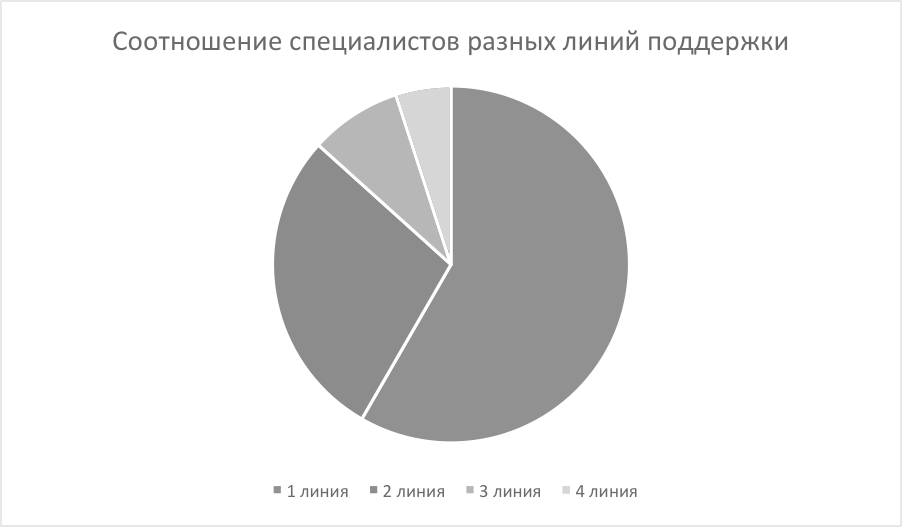
\includegraphics [scale=0.8] {ITSMTeamComposition}
  \caption{Диаграмма состава команд} 
  \label{img:ITSMTeamComposition}  
\end{figure}

Работа специалистов первой линии поддержки состоит из множества рутинных и простых задач. На рисунке \ref{img:EngineerTasks} показано соотношение разных типов проблем, встречающихся во время работы службы поддержки, в таблице \ref{IncidentDescription} приведена расшифровка типов. Данные подготовлены на основе анализа работы команд \icl.


\begin{figure} [h] 
  \center
  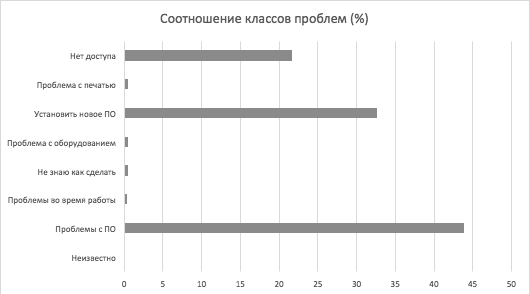
\includegraphics [scale=1.0] {EngineerTasks}
  \caption{Диаграмма соотношений типов проблем} 
  \label{img:EngineerTasks}  
\end{figure}



\begin{longtable}{|p{6cm}|p{10cm}|}
 \caption[Категории инцидентов в области удаленной поддержки инфраструктуры]{Категории инцидентов в области удаленной поддержки инфраструктуры}\label{IncidentDescription} \\ 
 \hline\multicolumn{1}{|c|}{\textbf{Категория}} & \multicolumn{1}{c|}{\textbf{Описание}} \\ \hline 
\endfirsthead
\multicolumn{2}{c}%
{{\bfseries \tablename\ \thetable{} -- продолжение}} \\
\hline\multicolumn{1}{|c|}{\textbf{Категория}} & \multicolumn{1}{c|}{\textbf{Описание}} \\ \hline 
\endhead
\endfoot

\hline \hline
\endlastfoot
  \hline
Проблема с ПО	& Проблема при запуске ПО на компьютере. Решается переустановкой \\
  \hline
Проблемы во время работы  & Проблема с функционированием программного обеспечения\\
    \hline
Как сделать & Запрос на инструкцию по работе с тем или иным компонентом рабочей станции \\
      \hline
Проблема с оборудованием  & Неполадки на уровне оборудования \\
  \hline
Установить новое ПО       & Требование установки нового программного обеспечения \\
  \hline
Проблема с печатью        & Установка принтера в систему \\
    \hline
Нет доступа               & Нет доступа к общим ресурсам \\
 
\end{longtable}

Как показывают исследования, решение части задач может быть автоматизировано. Если это будет сделано,  специалисты получат дополнительное время для решения более сложных задач. \par

\textbf{Применение моделей теории массового обслуживания}\par
Рассмотрим модель данной системы в разрезе теории массового обслуживания (ТМО). Она может быть выражена в виде входящего потока заявок (инцидентов), очереди и нескольких агентов (специалистов, автоматизированных систем). 
Важно отметить, что на время обработки заявки агент блокируется и не может принимать новые заявки. На рисунке \ref{img:mass_service} представлена модель системы массового обслуживания в ИТ, в которой использованы следующие обозначения рассматриваемых величин $\lambda$ --- интенсивность входящего потока;
$\alpha$ --- доля заявок, для которых время в очереди превышает $max(T_q)$;       
$\mu$ --- величина, обратная среднему времени нахождения заявки у агента;
n --- число агентов;
$T_q$ --- время нахождение заявки в очереди в часах;
SLA --- уровень обслуживания (1-$\alpha$), доля заявок, для которых время в очереди не превышает $max(T_q)$. $T_p$ --- время удовлетворения заявки;
 $\alpha_n$ --- количество заявок;
 $T_{qp}=T_q+T_p$ --- время прохождения заявки через систему;
 $S(\mu)= \frac{R_p}{\mu} $ --- средняя стоимость выполнения одной заявки;
 $R_p$ --- средняя стоимость часа работы специалиста (выводится далее).

  
\begin{figure} [h] 
  \center
  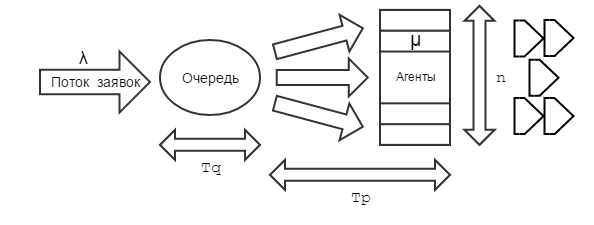
\includegraphics [scale=0.8] {mass_service}
  \caption{Модель системы массового обслуживания в ИТ.} 
  \label{img:mass_service}  
\end{figure}

Существует несколько подходов решения задач ТМО: 
\begin{itemize}
	\item Аналитическое решение для простейших систем, которое позволяет выразить $T_q (t)$ через $\lambda$, $\mu$ и $n$;
	\item Решение с помощью имитационного подхода, где строится гистограмма $T_q (t)$, по которой оценивается достаточность $n$ для обеспечения SLA;
	\item Решение с помощью эконометрического подхода, которое подходит для систем с достаточно большим $n$. В таких системах возможно оценить $T_q (t)$ по имеющейся статистике.
\end{itemize} \par
В \cite{TMO} на основе комбинации формулы Эрланга, модели Энгсета и модели Полячека~--~Хинчина 
построена формула для решения задач ТМО на основе аналитического подхода путем нахождения распределения вероятностей для $T_qp$. Основной же задачей этой работы является прогнозирование необходимых ресурсов для максимизации $SLA$~ ($SLA=1-\alpha$). 
В данной диссертации ставится задача минимизации $T_{qp}$, $S(\mu)$ и динамического выделения ресурсов. На основе  статистики, собранной в компании \icl,~ был подсчитан следующий коэффициент $T_{qp}=47,9$ при $n=6$; $SLA=0,82$; $\alpha=0,18$;  $\alpha_n=2920$. 
Для анализа потока заявок в данном случае лучше использовать имитационный подход, так как $n$ слишком мало. На рисунке \ref{img:LAMBDAAV} представлен средний поток заявок по часам, посчитанный на основе собранной статистики. На нем наглядно видно, как изменяется поток с течением дня. Пик обращений от пользователя приходится на промежуток между 13:00 и 16:00.

\begin{figure} [h] 
  \center
  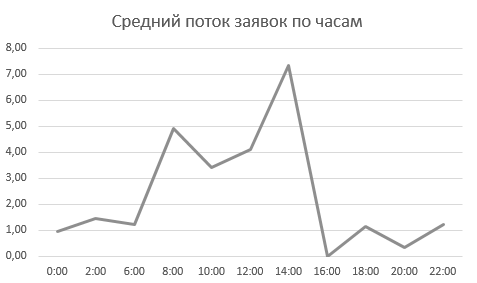
\includegraphics [scale=1.0] {LAMBDAAV}
  \caption{Средний поток заявок по часам.} 
  \label{img:LAMBDAAV}  
\end{figure}


\textbf{Оценка стоимости работы специалиста}\par По данным аналитики портала SuperJob \cite{SuperJob}, в Казани средняя зарплата системного администратора с опытом работы в 2014 году составляла 30 – 35 тыс. руб. (с учетом 21 рабочего дня в месяце~--- 179--208 руб. в час). В соответствии с действующим российским законодательством \cite{FiscalCodecs} расходы компании на одного работника определяются по формуле
\[
L = R + R*(F_1 +F_2+F_3),
\]
где $R$~--- выплата человеку в час, $F1$~--- НДФЛ 13\%, $F2$~--- совокупность отчислений в ФБ (6\%), ПФР (14\%), ТФОМС (2\%), ФФОМС (1,1\%), ФСС (2,9\%), $F3$~--- налог на прибыль (20\%). Таким образом, расходы компании на сотрудника варьируются от 285 до 314 руб. в час, а за 8-ми часовой рабочий день – от 2280 до 2512 руб. Далее, аренда выделенного сервера (такого, например, как Xeon X3, 1.7 GHz, 8GB RAM, 256GB SSD) стоит 8 900 руб./мес. (см. \cite{TimeWeb}) (53 рубля за 1 час, с учетом 8-ми часового рабочего дня $R_p=53$). Но сервер может работать 24 часа в сутки за исключением простоев на обслуживание, которые обычно составляют не более 5\% времени. \par

 Итого: сервер работает 478,8 часов в месяц. С этой точки зрения эксплуатация сервера будет стоить 18,5 руб. в час ($R_p=18,5$). Один сервер в своем быстродействии может заменить несколько специалистов при решении соответствующих задач. Чтобы решение было экономически эффективным, необходимо, чтобы оно сокращало расходы как минимум на 30\% (по данным \icl). \par 
 
 Подсчет на основе стоимости часа и пропорции показывает, что работа специалиста~--- это 6\% работы виртуального агента, т.е. сервера (без учета работы сервера параллельно над несколькими задачами). Таким образом, уровень разрешения инцидентов системой в 30\% выполнит требования по прибыли примерно на 111\%.

\textbf{Предпосылки развития изучаемой предметной области}\par 
Основной тенденцией в развитии области удаленной поддержки ИТ-инфраструктуры являются попытки удешевить и улучшить стоимость предоставления услуг \cite{OutsourceEff}. \par
Компании, работающие на этом рынке, вкладывают большие средства в автоматизацию. Кроме того, современное развитие науки и техники, точнее, вычислительных мощностей \cite{SuperComputer} позволяет провести автоматизацию даже самых наукоемких процессов. Дальнейшей перспективой развития области удаленной поддержки ИТ-инфраструктуры является замена человеческих специалистов автоматизированными системами. Разработки в этом направлении ведут многие компании, например, компания HP, которая имеет свою систему регистрации различных инцидентов \cite{HPOpenView} и сейчас ведет работу над ее автоматизацией. В качестве некоторого сравнения можно провести параллель происходящего процесса с промышленной революцией XVIII–XIX веков (см., например, \cite{IndustrialRev}). \par
\textbf{Обзор исследований в изучаемой предметной области}\par Область исследования, с которой связана диссертация, является комплексной и включает в себя различные направления работ, в частности, создания различных интеллектуальных систем. Сфера применения интеллектуальных систем обширна, например, в Институте Чиная (Индия) Е. Джубилсоном и П. Дханавантини ведутся исследования интеллектуальных систем обработки запросов пользователей в области телекоммуникаций \cite{CHIN-1}, а в университете Ганновера (Германия) Р. Брунс и Дж. Данкель разрабатывают интеллектуальные системы для обработки запросов в службу спасения с целью уменьшения времени реакции на происшествие \cite{Dunkel}. В Санкт-Петербургском государственном университете под руководством В.И. Золотарева проводится оценка эффективности службы информационной поддержки в Вычислительном центре СПбГУ \cite{SPB}. В Сингапуре С. Фу и П. Леонг проведен анализ эффективности ИТ-службы поддержки крупной компании и показана возможность автоматизации ряда процессов \cite{SING}.\par
Исследования в области интеллектуальных систем повышения эффективности ИТ-службы предприятия ведутся также лидерами отрасли: компаниями HP \cite{HPOpenView} и IBM \cite{WATSON-PO}. Например, известна многоцелевая интеллектуальная система IBM Watson, разработкой и исследованием которой занимается группа под руководством профессора А. Гоэля (США--Китай).  \par   

Еще одно из направлений исследований в области обработки естественного языка составляет подход GATE \cite{GATE-1}, который активно развивается в университете Шеффилда (Великобритания) под руководством Г. Каллаган, Л. Моффат и С. Сзаз. Другое направление~--- это семантический поиск, исследования в этой области также активно ведутся в университете Шеффилда, в частности, выработан подход "Mimir"\,, который реализует возможности поиска по принципу «поиск и открытие» \cite{MIMIR}. Для организации поиска решений в соответствии с запросами пользователей в таких системах используются онтологии, например, широко применяется подход, предложенный С. Дей и А. Джеймс из Калифорнийского университета (США), основанный на применении деревьев тегов в онтологии \cite{ONTCON}. \par
Для придания интеллектуальной системе гибкости необходимо дать ей возможность проводить логические рассуждения. Одной из ведущих организаций в этом направлении исследований является консорциум OpenCog \cite{OpenCog} (США). Этими работами руководит Бен Герцель (председатель Artificial General Intelligence Society и OpenCog Foundation)~--- один из мировых лидеров в области искусственного интеллекта. Исследования в области машинной логики также ведутся в рамках проекта NARS \cite{NARS} под руководством профессора университета Темпла (США) Пея Вонга. \par 

Интерес к области интеллектуальных систем обработки информации можно, в частности, оценить как количество публикаций за последние годы, процитированных в базе данных Scopus,~--- с 2004 года в среднем оно составило около 1010 в год. \par
\textbf{Стандарты, используемые в области ИТ-аутсорсинга: ITIL и ITSM} \par
В области ИТ-аутсорсинга есть несколько готовых стандартов ведения работ, одним из которых является библиотека ITIL. Этот стандарт описывает лучшие практики организации работ в области ИТ-аутсорсинга. Используемый в библиотеке подход соответствует стандартам ISO 9000 (ГОСТ Р ИСО 9000) \cite{ITIL1, ITIL2, ITIL3}.
Наличие стандартов диктует унифицированность как постановки проблем, так и алгоритмов решения, а также способствует возможности частичной или в некоторых случаях полной автоматизации решения проблем. \par
\clearpage


\section{Сравнительный анализ систем регистрации и устранения проблемных ситуаций} \label{sect3_2}
\textbf{HP OpenView} \cite{HPOpenView, HP1, HP2, HP3} является комплексным программным решением по мониторингу ИТ-инфраструктуры предприятия и имеет множество модулей. На рисунке \ref{img:hpopenview} представлен вид системы, которая обладает широким спектром возможностей: мониторинг \cite{HP4, HP5}; регистрация инцидентов; управление системами. Система не поддерживает: понимание и формализацию запросов; автоматическое устранение проблемы на основе формализации запроса.

\begin{figure} [h] 
  \center
  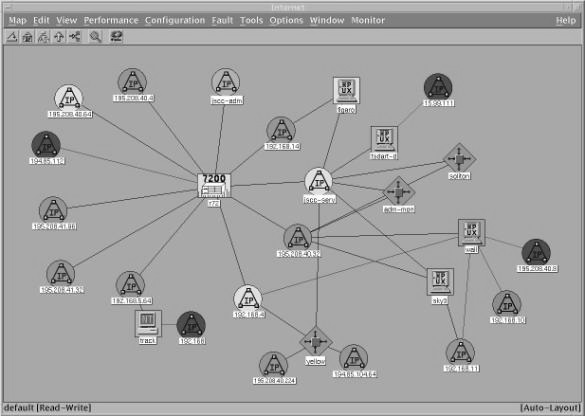
\includegraphics [scale=1.0] {hpopenview}
  \caption{HP OpenView (материал из Wikipedia)} 
  \label{img:hpopenview}  
\end{figure}

Система \textbf{ServiceNOW}\footnote{Система ServiceNOW \url{http://www.servicenow.com/}}~--- средство автоматизации сервиса. На рисунке \ref{img:svnow} представлен вид этой системы, которая предоставляет следующие возможности: регистрация инцидентов и создание цепи их обработки. Система не поддерживает: понимание и формализацию запросов; автоматическое исправление проблемы на основе формализации запроса. Система широко используется в ИТ-инфраструктуре CERN \cite{SN1, SN2} для регистрации инцидентов и их решения.

\begin{figure} [h] 
  \center
  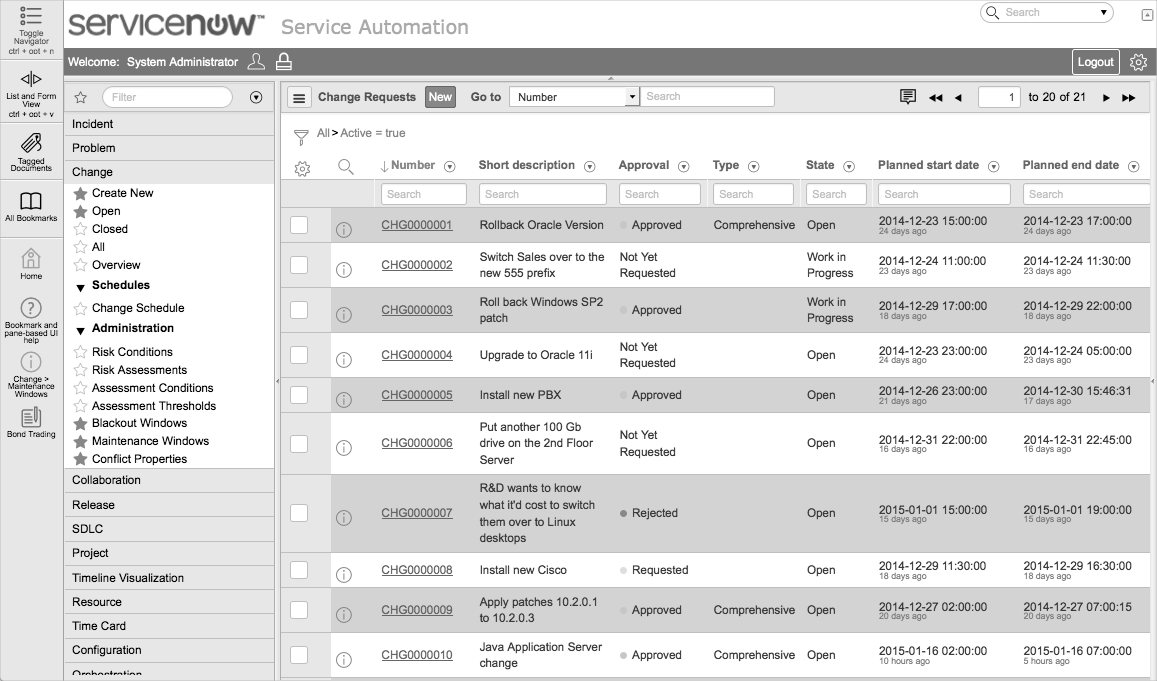
\includegraphics [scale=0.3] {svnow}
  \caption{Service NOW (материал из http://wiki.servicenow.com/)} 
  \label{img:svnow}  
\end{figure}

\textbf{IBMWatson}~--- это вопросно-ответная система, которая поддерживает понимание и формализацию запросов и поиск решений. Система не поддерживает автоматическое разрешение проблемы на основе формализации запроса. Система широко используется в медицине для постановки диагнозов болезней \cite{IBM1, IBM2, IBM3, IBM4} и реализует базовые принципы искусственного интеллекта \cite{IBM5, IBM6}. Ее разработка велась под суперкомпьютер IBM Deep Blue \cite{IBM7} группой под руководством профессора А. Гоэля. На рисунке \ref{img:Watson-Analytics} представлен общий вид этой системы. \par


\begin{figure} [h] 
  \center
  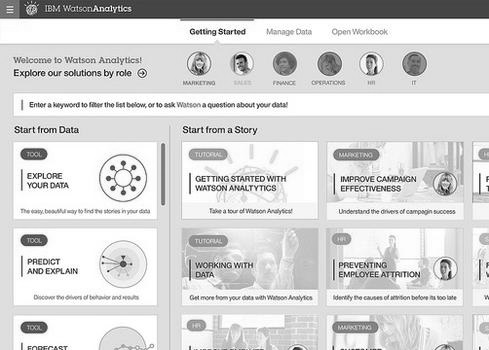
\includegraphics [scale=1.0] {Watson-Analytics}
  \caption{Пример работы системы Watson (материал из http://www.informationweek.com/)} %http://www.informationweek.com/cloud/software-as-a-service/ibm-watson-data-analysis-service-revealed/d/d-id/1315769
  \label{img:Watson-Analytics}  
\end{figure}

Кроме того, известны следующие дополнительные способы и системы автоматизации разрешения проблемы пользователя:
\begin{itemize}
	\item Обработка инцидентов посредством регулярных выражений. В таком решении нет гибкости, так как обработка идет путем поиска ключевых слов вне контекста. Метод регулярных выражений частично используется для обработки естественного языка, поиска  \cite{REG1}, диагностики активных систем \cite{REG2}, анализа поведения функций \cite{REG4}, обработки данных в системе eDiscovery \cite{REG5}, в разработке способов программирования \cite{REG3};
	\item Обработка инцидентов при помощи скриптов~--- автоматизируются лишь рутинные операции.
\end{itemize} \par
На данный момент времени ни одна из описанных систем в полной мере автоматически не разрешает запросы пользователей: не фиксирует их, не проводит анализ, не ищет решение, не применяет решение и не дает обратной связи пользователю. Каждая система в той или иной мере реализует те или иные функции, но системы, которая реализует их все, пока не существует. \par

Для того чтобы создать модель системы, необходимо определить требования к ней или критерии, соответствие которым будет служить одним из доказательств состоятельности системы наряду с экспериментальными результатами. \par

Перечисленные ниже требования сформированы, исходя из возможностей специалистов службы поддержки, а также анализа проблем, которыми они занимаются. Большинство инцидентов~--- тривиальные и типичные, но все они разные. Для человека проблемы ”Please install Firefox” и ”Please install Chrome” идентичны, но с точки зрения формализации это не так~--- общее в них можно найти, взглянув на обобщение различающейся части: Firefox и Chrome являются пакетами программного обеспечения. \par 
Чтобы понять, каким требованиям должны соответствовать интеллектуальная система регистрации и анализа проблемных ситуаций в ИТ-области, нужно понять, что делает специалист службы поддержки. Такой специалист регистрирует проблему, анализирует, ищет решение, проводя логические рассуждения и фиксируя в памяти удачное решение, и решает проблему. Итак, чтобы обеспечить полностью автоматическое разрешение инцидентов, интеллектуальная система регистрации и анализа проблемных ситуаций в ИТ-области должна соответствовать следующим критериям: осуществлять мониторинг ИТ-инфраструктуры пользователя; регистрировать инциденты; создавать цепи обработки (Workflow) инцидента; понимать и формализовать запросы пользователя на естественном языке; искать решение и применять найденное решение; обучаться алгоритму разрешения инцидента; уметь проводить логические рассуждения (обобщение, специализация, синонимичный поиск). \par
Из этого списка требований к системе важно выделить формализацию запросов на естественном языке. Ниже приведены результаты анализа разработок в области формализации запросов на естественном языке. 


\section{Сравнительный анализ методов и комплексов обработки текстов на естественном языке}


\subsection{Обработка эталонных текстов} \label{sect2_1}
В данном разделе проведен обзор обработчиков естественного языка. За основу были взяты инциденты, выгруженные из систем поддержки ИТ-инфраструктуры \icl. В силу специфики предметной области (информационные технологии) основным языком был выбран английский язык. Был сформирован список из типичных эталонных фраз, на которых тестировались обработчики естественного языка. Фразы были выявлены путем анализа существующих отчетов об инцидентах. Примерами инцидентов являются следующие запросы.\par
\textbf{Инцидент 1}.
\textit{
User had received wrong application. User has ordered Wordfinder Business Economical for her service tag 7Q4TC3J, there is completed order in LOT with number ITCOORD-18125. However she received wrong version, she received Wordfinder Tehcnical instead of Business Economical. Please assist (Пользователю было установлено неверное приложение. Пользователь заказал приложение "Wordfinder Business Economical"\  для ее запроса номер 7Q4TC3J. По нашим данным запрос выполнен, номер результата ITCOORD-18125. Однако, он получил неверную версию~--- он получил приложение "Wordfinder Tehcnical"\  вместо "Wordfinder Business Economical". Пожалуйста, помогите).\footnote{Здесь и далее в переводе оригинальные синтаксические, грамматические и стилистические ошибки сохранены, дабы продемонстрировать сложность формализации запросов на естественном языке.}
}\par
\textbf{Инцидент 2}.
\textit{
Laptop~--- user has almost full C:\ but when he looks in the properties of the files and folders on C:\ they are only 40~Gb and he has a 55~Gb drive (Ноутбук~--- диск C:\ пользователя переполнен, но он посмотрел свойства C:\ и увидел, что имеется только 40~Gb, хотя пользотель установил накопитель на 55~Gb).
}\par
\textbf{Инцидент 3}.
\textit{
User cannot find Produkt Manageron start menu. Please reinstall (Пользователь не может найти Produkt Manageron в меню "Пуск". Пожалуйста, переустановите). 
}\par
\textbf{Инцидент 4}.
\textit{
User needs to have pdf 995 re-installed please (Пользователю нужно переустановить "pdf 995").
}\par

При анализе этих запросов были использованы следующие обработчики естественного языка: Open NLP \cite{OpenNLP}, Relex\cite{OpenCogRelex}, StanfordParser \cite{StanfordParser}. Результат их работы оценивался при помощи метрик, представленных в таблице \ref{Metrics}, а полученные результаты приведены на рисунке \ref{img:ParserComp}. 

\begin{longtable}{|p{2cm}|p{6cm}|p{8cm}|}
 \caption[Таблица метрик]{Таблица метрик}\label{Metrics} \\ 
 \hline
 
 \multicolumn{1}{|c|}{\textbf{Метрика}} & \multicolumn{1}{c|}{\textbf{Описание}} & \multicolumn{1}{c|}{\textbf{Формула}} \\ \hline 
\endfirsthead
\multicolumn{2}{c}%
{{\bfseries \tablename\ \thetable{} -- продолжение}} \\
\hline\multicolumn{1}{|c|}{\textbf{Метрика}} & \multicolumn{1}{c|}{\textbf{Описание}} & \multicolumn{1}{c|}{\textbf{Формула}}  \\ \hline 
\endhead
\endfoot

\hline \hline
\endlastfoot
  \hline

Precision	& Точность & 
$$ 
P=\frac{tp}{tp+fp},
$$ где $P$~--- precision, $tp$~---  успешно обработанные слова, $fp$~--- ложно успешные \\
 \hline
Recall	& Чувствительность & 
$$ 
R=\frac{tp}{tp+fn},
$$ где $R$~--- recall, $tp$~--- успешно обработанные слова, $fn$~--- ложно неуспешные \\
 \hline
$F$	& $F$~--- measure (результативность) & 
$$ 
F=\frac{P*R}{P+R},
$$ где $P$~--- precision, $R$~--- recall.   \\
 
\end{longtable}

\begin{figure} [h] 
  \center
  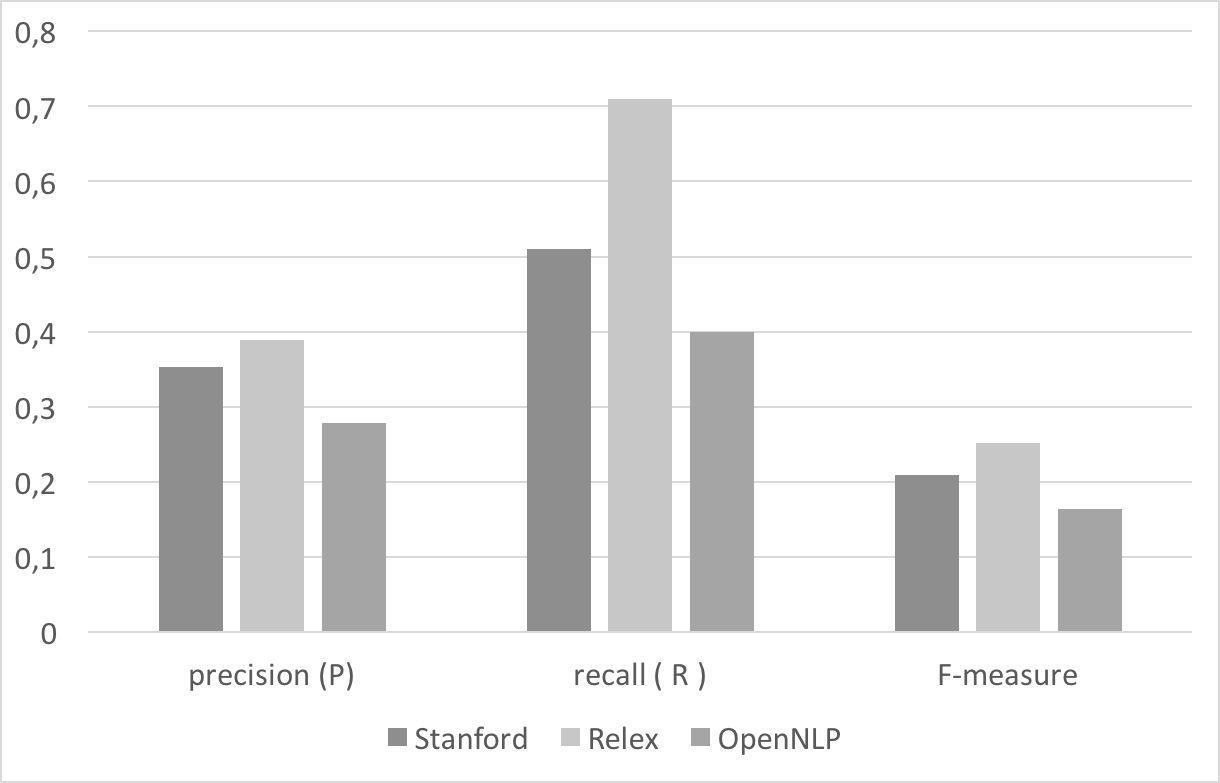
\includegraphics [scale=0.8] {ParserCompare}
  \caption{Результаты обработки текстов} 
  \label{img:ParserComp}  
\end{figure}

Из диаграммы \ref{img:ParserComp} видно, что наилучшие результаты показывает обработчик Relex\cite{OpenCogRelex}. После анализа необработанных инцидентов у всех обработчиков были выявлены проблемы двух типов:
\begin{enumerate}
	\item невозможность корректировки простых грамматических ошибок, связанных с пропущенными пробелами или неверным форматированием (ошибки первого типа);
	\item полисемия, например, слово please интерпретировалось как глагол, хотя является по смыслу «вводным словом» (ошибки второго типа).
\end{enumerate}	\par

Несмотря на хорошие результаты~--- 63\% успешно разобранных предложений, ошибки первого и второго типов серьезно ухудшают результат. Эффективность разбора предложений в 63\% случаев недостаточна для успешной работы системы. Чтобы улучшить показатель, был разработан комплекс мер для устранения ошибок первого и второго типов.
	
 
\subsection{Исправление ошибок первого и второго типов} \label{sect2_2}
Чтобы разрешить проблемы, связанные с ошибками первого и второго типов, была проведена предварительная обработка текста, состоящая из 2-х фаз: комплексная корректировка~--- для ошибок первого типа; обработка при помощи внутренней базы знаний~--- для ошибок второго типа. 
Чтобы избавиться от орфографических, грамматических и синтаксических ошибок, был сконструирован составной корректировщик, который имеет модульную структуру и осуществляет корректировку последовательно в рамках выбранной области знаний (например, одного проекта). В результате были сконструированы модули корректировки: Google API~--- модуль подключения к открытым системам Google для использования их алгоритмов корректировки; After the Deadline~--- модуль, использующий открытый программный продукт After the Deadline для исправления текстов. 

Таким способом удалось исправить большинство ошибок, связанных с синтаксисом, грамматикой и орфографией в рамках выбранной области (корректировка ошибок в ограниченной области гораздо проще, чем универсальная корректировка). Также удалось исправить ошибки неверного написания: наличия лишних пробелов, пропуска запятых и точек в виду лаконичности входной информации. Необходимо отметить, что входная информация представляет собой простые предложения в рамках терминологии одной области знаний (ИТ, специфические термины, которые используются только на этом проекте), что значительно упрощает корректировку ошибок. По-прежнему осталась проблема обработки неверной интерпретации слов в тексте (полисемии). \par

Для корректировки ошибок второго типа был сконструирован модуль для обработчика естественного языка Relex, который разбивал стандартный процесс обработки на «предобработку» и «обработку». Стадия «обработки» включает в себя такой же алгоритм работы, как был до этого в модуле Relex, а стадия «предобработки» проверяет входные данные (слово или предложение) на предмет его вхождения во внутреннюю базу знаний, и если таковое имеется, то приложение передает соответствующие корректировки обратно в модуль. Например, Relex во фразе "please install firefox"\ считает, что "please"\ --- это глагол, поэтому в базе знаний нашей системы отмечено, что "please"\ --- это форма вежливости (проблема полисемии), тем самым Relex больше не интерпретирует "please"\ как глагол в выбранной области знаний (то есть для всех случаев).


\subsection{Сравнение средств обработки русского и английского языков} \label{sect2_3}
Средства обработки естественного языка принято относить к большому классу средств NLP~--- Natural Language Processing \cite{NLP}. Для английского языка существует множество открытых средств обработки этого языка, для русского языка найти их гораздо сложнее. Рассмотрим архитектуру средств обработки естественного языка на примере популярного комплекса обработки~--- OpenCog Relex \cite{OpenCogRelex}. \par
OpenCog Relex использует результаты работы открытого компонента для лексического анализа под названием Link Grammar \cite{linkgrammar}. Он поддерживает множество языков: английский, русский, турецкий, немецкий \etc\  В качестве формата вывода Relex использует синтаксис Link Grammar и преобразует его в формат связей, как показано в примере 1. Разбор примера приводится далее. 

\textbf{Пример 1}. User is unable to start KDP web, please reinstall Java.\\
\textbf{Результат} 
\begin{lstlisting}
_obj(start, KBP)
pos(start, verb)
inflection-TAG(start, .v)
tense(start, present)
pos([web], WORD)
noun_number(KBP, singular)
definite-FLAG(KBP, T)
pos(KBP, noun)
_advmod(reinstall, please)
pos(reinstall, verb)
inflection-TAG(reinstall, .v)
tense(reinstall, present)
pos(please, adv)
inflection-TAG(please, .e)
noun_number(Java, singular)
definite-FLAG(Java, T)
pos(Java, noun)
pos(., punctuation)
_obj(,, Java)
pos(,, verb)
tense(,, infinitive)
HYP(,, T)
_to-do(unable, ,)
pos(unable, adj)
inflection-TAG(unable, .a)
tense(unable, present)
pos(to, prep)
inflection-TAG(to, .r)
pos(be, verb)
inflection-TAG(be, .v)
_predadj(User, unable)
noun_number(User, singular)
definite-FLAG(User, T)
pos(User, noun)
\end{lstlisting}




Далее проведем разбор слова start. В результате мы получим несколько отношений:
\begin{itemize}
	\item pos(start, verb)~--- start глагол;
	\item tense(start, present)~--- время настоящее;
	\item inflection-TAG(start, .v)~--- метод обозначения на схеме (индекс).
\end{itemize} \par
Остальные обработчики пока не поддерживают русский язык. Существуют открытые проекты, но они еще недостаточно развиты. Таковым является, например, русский словарь для LinkGrammar \footnote{\url{http://www.abisource.com/projects/link-grammar/russian/}}, но он не доступен для скачивания. 




\section{Выводы по главе 1}
В данной главе рассмотрены существующие на данный момент интеллектуальные системы регистрации и анализа проблемных ситуаций, возникающих в процессе функционирования ИТ-инфраструктуры предприятия.
 В таблице \ref{Comparsion} приведены сводные данные по системам. По ним можно сказать, что ни одна из рассмотренных систем полностью не реализует все необходимые функции для интеллектуальной системы разрешения проблемных ситуаций в ИТ-инфраструктуре предприятия. В главе 1 также выработаны критерии сравнения обработчиков естественного языка и выполнен анализ средств обработки естественного языка. По полученным показателям эффективности было решено использовать OpenCog Relex.

\begin{longtable}{|p{6cm}|p{0.5cm}|p{0.5cm}|p{0.5cm}|}
 \caption[Сравнительный анализ функциональности существующих решений]{Сравнительный анализ функциональности существующих решений}\label{Comparsion} \\ 
 \hline
 
 \multicolumn{1}{|c|}{\textbf{Сравнительный пункт}} & \multicolumn{1}{c|}{\textbf{HP Open View}} & \multicolumn{1}{c|}{\textbf{ServiceNOW}} & \multicolumn{1}{c|}{\textbf{IBM Watson}} \\ \hline 
\endfirsthead
\multicolumn{2}{c}%
{{\bfseries \tablename\ \thetable{} -- продолжение}} \\
\hline \multicolumn{1}{|c|}{\textbf{Сравнительный пункт}} & \multicolumn{1}{c|}{\textbf{HP Open View}} & \multicolumn{1}{c|}{\textbf{ServiceNOW}} & \multicolumn{1}{c|}{\textbf{IBM Watson}}  \\ \hline 
\endhead

\hline \multicolumn{4}{|r|}{{Продолжение следует}} \\ \hline
\endfoot

\hline \hline
\endlastfoot
\hline
   Мониторинг & Да & Да & Да \\
   \hline
   Регистрация инцидентов & Да & Да & Да\\
   \hline
   Управление системами & Да & Нет & Нет \\
   \hline 
   Создание цепи обработки (Workflow) инцидента & Да & Да & Нет \\
   \hline 
   Понимания и формализация запросов на естественном языке & Нет & Нет & Да \\
   \hline 
   Поиск решений & Нет & Нет & Да \\
   \hline 
   Применение решений & Нет & Нет & Нет \\
   \hline
   Обучение разрешению инцидента & Нет & Нет & Да \\
   \hline
   Умение проводить логические рассуждения: генерализацию, специализацию, синонимичный поиск & Нет & Нет & Нет \\
     
\end{longtable}
\clearpage
           % Глава 1
\chapter{Модель интеллектуальной системы принятия решений для регистрации и анализа проблемных ситуаций в ИТ-инфраструктуре предприятия} \label{chapt3}

В данной главе рассмотрены модели, которые были изучены и использованы при создании системы принятия решений для регистрации и анализа проблемных ситуаций в ИТ-инфраструктуре предприятия. Отметим, что работа над системой велась с 2011 года, за истекшее время было создано три рабочих версии прототипа системы, реализующих различные модели мышления. \par
Созданными и испытанными моделями, использованными при создании системы принятия решений для регистрации и анализа проблемных ситуаций в ИТ-инфраструктуре предприятия, являются:
 \begin{itemize}
	\item модель Menta 0.1, построенная с использованием деревьев принятия решений;
	\item модель Menta 0.3, построенная с использованием генетических алгоритмов \cite{ArtificialIntelligence} ;
	\item модель TU 1.0, основанная на модели мышления Марвина Мински  \cite{EmotionMachine}.
\end{itemize}

Модель, построенная на базе нейронных сетей (поддерживающая обучение), была отброшена на предварительной стадии оценки, так как она предъявляет большие требования к производительности (скорости работы и требуемых ресурсов)\cite{NEURAL}, что в свою очередь порождает высокую стоимость. Далее каждая модель будет рассмотрена подробно.

%====================

%====================
\section{Построение модели Menta 0.1 с использованием деревьев принятия решений} \label{sect3_1}
Данная модель была одной из первых, которые были апробированы. Она основана на деревьях принятия решений \cite{DTREE}, которые широко используются в вопросно-ответных системах \cite{DC1, DC2, DC3}. При построении модели использованы компоненты, реализующие обработку запросов на естественном языке, поиск решения, применение найденного решения, хранение в базе знаний.\par
Система ориентирована на выполнение таких простых команд, как, например, «Добавить поле в форму». Основные функции модели представлены следующими потоками: получение и формализация запроса; поиск решения при помощи деревьев принятия решений; изменение приложения согласно запросу; генерация и компиляция приложения. Рассмотрим подробнее, как устроена система. Начнем с того, как в системе представлены данные.

\subsection{База знаний на основе OWL}
Для представления данных в системе была использована база знаний, построенная на основе OWL-файла (см. \cite{OWL}). С помощью редактора Protege \cite{Protege} в базу вводились начальные данные о целевом приложении (приложении, которое будет модифицироваться системой согласно запросам пользователей) в виде семантической сети. В качестве такого приложения была создана система, которая вела учет заказов пользователя на покупку того или иного товара в интернет-магазине. \par

 На рисунке \ref{img:order-owl} представлен один из программных классов (согласно терминологии ООП \cite{Meyer}) этой системы~--- Order~--- в формате OWL. Этот класс отвечает за обработку заказов. Слева отображены супер классы (классы-предки), к которым он привязан. Например, класс BLL относится к бизнес-логике приложения, Module~--- отдельный модуль в рамках системы. Справа представлены свойства класса, а их описания приведены в таблице \ref{OrderPropertyDescription}. С помощью предикатов определяется поведение свойства: создать файл, создать новое поле. В таблице \ref{Predicates} представлено описание иерархии предикатов. На рисунке \ref{img:CreateCustomer} представлен класс CreateCustomer в OWL, в который входит описание всех необходимых свойств для генерации файла исходного кода на языке Java.

\begin{figure} [h] 
  \center
  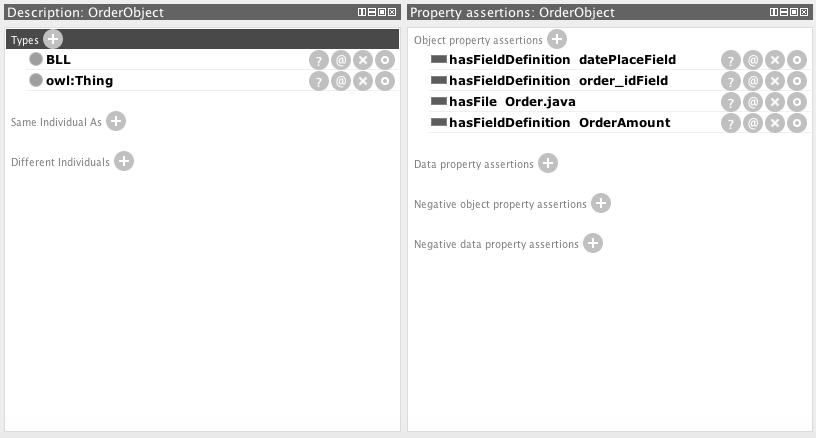
\includegraphics [scale=0.7] {OrderOWL}
  \caption{Представление класса Order в OWL. Визуализация Protege} 
  \label{img:order-owl}  
\end{figure}


\begin{table} [htbp]
  \centering
  \parbox{15cm}{\caption{Описание свойств класса Order в OWL}\label{OrderPropertyDescription}}
%  \begin{center}
  \begin{tabular}{| p{3cm} | p{4cm} | p{8cm} |}
  \hline
 \textbf{Свойство} & \textbf{Предикат} & \textbf{Описание} \\
  \hline
    OrderAmount	& hasFieldDefinition & Поле: сумма заказа \\
  \hline
orderidField	& hasFieldDefinition & Поле: идентификатор заказа \\
  \hline
Order.java	& hasFile & Идентификатор имени файла для генерации \\
  \hline
datePlaceField	& hasFieldDefinition & Поле: время размещения заказа \\
  \hline
    \end{tabular}
%  \end{center}
\end{table}

\begin{table} [htbp]
  \centering
  \parbox{15cm}{\caption{Описание иерархии предикатов}\label{Predicates}}
%  \begin{center}
  \begin{tabular}{| p{5cm} | p{10cm} |}
  \hline
  
\textbf{Предикат} & \textbf{Описание} \\
  
    \hline
 hasFieldDefinition & Предикат, обозначающий свойство класса \\
  \hline
 hasMethodDefinition & Предикат, обозначающий функцию \\
  \hline
classDefinition & Обозначение класса \\
  \hline
database & Обозначение базы данных\\
  \hline
    \end{tabular}
%  \end{center}
\end{table}

\begin{figure} [h] 
  \center
  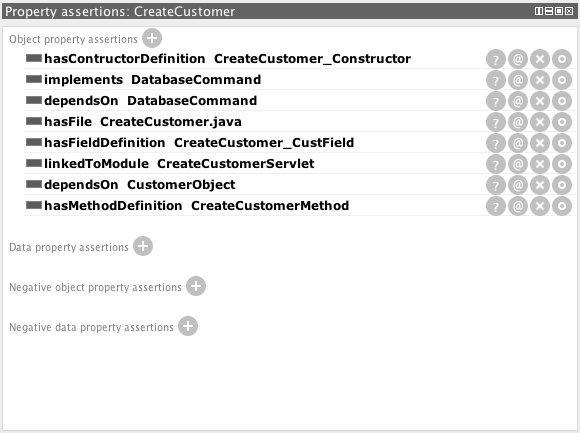
\includegraphics [scale=0.7] {CreateCustomer}
  \caption{Представление класса CreateCustiner в OWL. Визуализация Protege} 
  \label{img:CreateCustomer}  
\end{figure}
\clearpage
\subsection{Основные компоненты модели}
Основными компонентами модели являются: Request parser (Stanford parser); Генерация Action (Action Generator); Исполнение Action (Action Applier); Генерация приложения (Application Generator). \par
\emph{Request parser} формализует запрос на естественном языке. \emph{Action Generator} генерирует объект класса Action (который содержит описание требуемых над моделью приложения действий) из результатов работы, основываясь на Деревьях принятия решений \cite{DCFOREST} и базе данных. Основной задачей данного модуля является генерация имени, действия и поля. Модуль \emph{Action Applier} отыскивает объект в модели по данным от Action Generator и производит действие, кроме того, используя предикат dependOn, он производит модификацию всех зависимых классов. \par
 В модели поддерживается два типа Action: RemoveFieldAction (удаление поля), AddFieldAction (добавление поля). После завершения работы производится генерация целевого приложения на языке Java при помощи OWL-модели в модуле \emph{Application Generator}. На рисунке \ref{img:MentaUseCase} представлена UML-диаграмма последовательности для основного рабочего потока приложения: пользователь вводит в систему запрос "Add new field to Customer (Добавить новое поле в класс Customer)"; модуль StanfordParser вычленяет из запроса связи типа dobj (связь объекта и действия); модуль ActionGenerator создает на основе связей объект, описывающий список действий (далее~--- действие) над моделью, для получения требуемого результата; модуль ActionApplier, используя действие, изменяет модель приложения; модуль ApplicationGenerator применяет изменения к приложению. В результате у класса Customer (данный класс содержит набор свойств, необходимых для описания клиента магазина) появляется новое поле "New". \par
\begin{figure} [h] 
  \center
  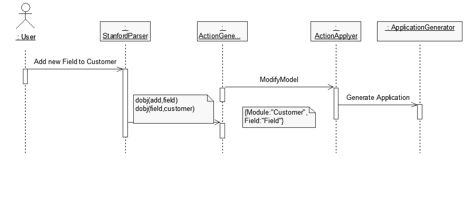
\includegraphics [scale=1.2] {MentaUseCase}
  \caption{UML-диаграмма последовательности для основного потока в модели Menta 0.1} 
  \label{img:MentaUseCase}  
\end{figure}
После проведения экспериментов было выявлено, что приложение не может использовать ранее найденные решения, абстрагируя их. Например, система знает, как произвести операцию добавления поля, но вот аналогичную операцию~--- добавить метод~--- сделать не может. Поиск решения также потребовал специального обучения: система не могла путем перебора информации в своей базе знаний найти решение.  В системе также не было возможности обучения. \par
После применения этой системы была предпринята попытка найти более универсальное решение. Результатом стало построение модели Menta 0.3, описанной ниже.

%===============================
\section{Модель Menta 0.3, построенная с использованием генетических алгоритмов} \label{chapt2}
В данную модель по сравнению с предыдущей были добавлены модуль логики для оценки решения и модуль генетических алгоритмов для генерации решения. Отметим, что генетические алгоритмы часто применяются в биологически инспирированных системах \cite{G1}, \cite{G3}. Кроме того, есть примеры их использования в системах поддержки принятия решений, однако эффективность таких систем не подтверждена \cite{G2}. В рамках модели Menta 0.3 были отработаны следующие основные компоненты будущей итоговой модели: критерии приемки (Acceptance Criteria); How-To~--- для хранения решений проанализированных проблем; формат данных OWL; использование логических вычислений для проверки решения. Система Menta 0.3 содержала внутри себя модель целевого приложения (как и Menta 0.1) и список решений тех или иных проблем (How-To). При помощи генетического алгоритма модель строила решение (How-To), проверяла его при помощи логического движка NARS \cite{NARS} на соответствие входным критериям приемки. С точки зрения генетических алгоритмов это~--- функция отбора особей из поколения \cite{GFITNESS}. 

\subsection{Основные компоненты модели}
Модель состоит из компонентов, представленных в Таблице \ref{ModulesMenta03}.

\begin{longtable}{|p{5cm}|p{11cm}|}
 \caption[Компонетны модели Menta 0.3]{Компонетны модели Menta 0.3}\label{ModulesMenta03} \\ 
 \hline
 
 \multicolumn{1}{|c|}{\textbf{Компонент}} & \multicolumn{1}{c|}{\textbf{Описание}}  \\ \hline 
\endfirsthead
\multicolumn{2}{c}%
{{\bfseries \tablename\ \thetable{} -- продолжение}} \\
\hline \multicolumn{1}{|c|}{\textbf{Компонент}} &
\multicolumn{1}{c|}{\textbf{Описание}}  \\ \hline 
\endhead


\endfoot

\hline \hline
\endlastfoot
 MentaController & Веб-служба \cite{WebService}, которая предоставляет интерфейс для общения с пользователем и остальными системами \\
  \hline
 SolutionGenerator & Модуль отвечает за генерацию решения. На вход он получает Acceptance Criteria. Основой является генетический алгоритм. Для него был выбран framework ecj \cite{ECJ}. Из всех возможных классов в базе знаний, отсеянных по классификатору, составляются паросочетания. К каждому паросочетанию применяется логическое суждение на основе AcceptanceCriteria (за это отвечает модуль ReasonerAdapter). В итоге паросочетание получает оченку в виде пары Frequency, Confidence (частота, вероятность). 
Таким образом находится наилучшее паросочетание. Если его показатель 1,1, то решение принимается, иначе отбрасывается (на данный момент установлен жесткий показатель).
SolutionGenerator включает в себя SolutionChecker, который включает в себя ReasonerAdapter.
 \\
  \hline
SolutionChecker & Проверка решения. Принимает на вход выбранные How-To, AcceptanceCriteria. Комбинирует их и передает ReasonerAdapter. \\
  \hline
ReasonerAdapter & Транслирует  How-To в термины NARS. NARS~--- non-axiomatic reasoning system \cite{NARS} (система логических суждений, разработанная профессором Пеем Вонгом). Принцип действия NARS~--- это всевозможная комбинация фактов. Каждый факт имеет свои частоту и вероятность. Их сочетанием получается композиция данных фактов.\\
  \hline
  Translator & Транслирует объекты базы знаний (знания) в отчеты. Последние бывают следующих типов: Solution Report; UML Report; Patch. В данной версии используется первый тип отчета. Он содержит описание на выбранном языке программирования решения, найденного системой.\\
  \hline
  Applicator & Данный модуль применяет решение к модели приложения, содержащейся в базе знаний. Также данная модель включает FileApplicator, который генерирует решение в виде файлов на выбранном языке программирования. \\
  \hline
  KBServer & База знаний приложения. Используется сервер non-SQL БД HypergraphDB. \\
  \hline
%  \end{center}
\end{longtable}
В предыдущей модели в качестве хранения данных использовался файл, что было неудобно в случае, если приложение работает параллельно с несколькими запросами. В системе Menta 0.3 был использован специальный сервер баз данных, речь о котором пойдет далее.

\subsection{База знаний на основе графов}
При реализации базы знаний (здесь и далее~--- KBServer) был создан промежуточный модуль доступа к данным (здесь и далее~--- DAO, Data Access Object), данный подход широко используется в проектировании программного обеспечения \cite{THREELAYERARCH}. Это позволяет максимально отделить реализацию KBServer от конкретного хранилища. \par 

\textbf{EntityManagerFactory}. Данный класс является входной точкой и создает объект, с помощью которого приложение осуществляет работу с базой знаний. Класс автоматически выбирает необходимые настройки для объекта. \par

\textbf{EntityManager}. Это основной класс для загрузки и хранения объектов из базы данных.\par

\textbf{Configuration}. Этот класс хранит такие параметры настройки базы данных, как физическое положение БД и максимальное количество подключений. \par 
\textbf{EntityTransaction}. Данный класс используется для управления транзакциями при доступе к объектам базы данных. \par
При выборе физического хранилища данных было проанализировано несколько хранилищ OWL-данных: OWLIM, SESAME и HG. Результаты их сравнения представлены в таблице \ref{DatabaseEngineComparison}.
\begin{longtable}{|p{6cm}|p{3cm}|p{3cm}|p{3cm}|}
 \caption[Сравнение скорости доступа к данным баз знаний]{Сравнение скорости доступа к данным баз знаний}\label{DatabaseEngineComparison} \\ 
 \hline
 
 \multicolumn{1}{|c|}{\textbf{}} & \multicolumn{1}{c|}{\textbf{Sesame}} & \multicolumn{1}{c|}{\textbf{OWLIM}} & \multicolumn{1}{c|}{\textbf{HG}} \\ \hline 
\endfirsthead
\multicolumn{2}{c}%
{{\bfseries \tablename\ \thetable{} -- продолжение}} \\
\hline \multicolumn{1}{|c|}{\textbf{}} & \multicolumn{1}{c|}{\textbf{Sesame}} & \multicolumn{1}{c|}{\textbf{OWLIM}} & \multicolumn{1}{c|}{\textbf{HG}} \\ \hline 
\endhead

\endfoot

\hline \hline
\endlastfoot
 \textbf{Единицы измерения} & \textbf{мс.} & \textbf{мс.} & \textbf{мс.} \\
  \hline
 предварительно скомпилированные запросы & 26 253 & 3 012 & 6 813 \\
  \hline
 без кеша & 30 545 & 1 122 & 9 045 \\
  \hline
 с кешем & 24 258 & 962 & 985 \\
%  \end{center}
\end{longtable}

Несмотря на то, что OWLIM дает лучшие результаты, был выбран HGDB, который предоставляет более широкие возможности доступа к данным, такие, например, как поддержка алгоритмов работы с графами.

%========================================
%========================================

\section{Модель TU 1.0, основанная на модели мышления Марвина Мински}
Следующим этапом разработки стала модель, построенная с применением теории Марвина Мински. Эта модель сохранила следующие основные концептуальные элементы предыдущих моделей и показала свою состоятельность на контрольных примерах: Acceptance Criteria; Обучение; Поиск и применение решения; Отсутствие обработки естественного языка. Данная модель является более универсальной и представляет собой верхнеуровневую архитектуру обработки запроса (мышления), где компонентами являются лучшие части предыдущих систем.
\subsection{Особенности модели мышления}
В 2006 году Марвин Мински опубликовал свою книгу "The emotion machine" \cite{EmotionMachine}, в которой предложил свой взгляд на систему мышления и памяти человека. В основу его теории легла парадигма триплета \triplet\ (далее \tripletshort), k-line (линия, которая связывает приобретенные знания, например, огонь~--- горячо) для сопоставления знаний. На рисунке \ref{img:csw} представлено схематичное изображение \tripletshort. \par
\begin{figure} [h] 
  \center
  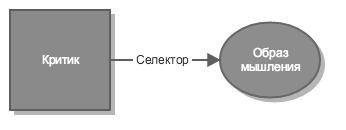
\includegraphics [scale=1.0] {csw}
  \caption{\triplet} 
  \label{img:csw}  
\end{figure}

\textbf{Критик} представляет собой определенный переключатель: внешние обстоятельства, события или иное воздействие. Например, «включился свет, и зрачки сузились», «обожглись и одернули руку». Критик активируется только тогда, когда для этого достаточно обстоятельств. Одновременно может активироваться несколько критиков. Например, человек решает сложную задачу, идет активация множества критиков: выполнить расчет, уточнить технические детали. Кроме того, параллельно может активироваться критик, сообщающий о необходимости отдыха.\par
\textbf{Селектор} занимается выбором определенных ресурсов, одним из которых является Образ мышления. \par
\textbf{Образ мышления}~--- это способ решения проблемы. Образ мышления может быть сложным и способен активировать других критиков. Например, размышляя над проблемой, специалист понимает, что нужно произвести полный перебор всех возможных комбинаций параметров, чтобы получить нужный результат, и тут он решает поискать готовое решение: а может кто-то уже сделал такой перебор, и можно будет использовать его результаты. Здесь «поиск готового решения» является критиком внутри образа мышления «поиск решения». \par

На рисунке \ref{img:csw_ex} представлена расширенная модель работы \tripletshort. Критик активирует Селектор, который активирует Образ мышления (овал). Последний в свою очередь может активировать нового Критика или же совершить определенные действия. Например, зажегся зеленый свет светофора, значит, можно переходить дорогу. Под ресурсами здесь понимается набор знаний из базы знаний: Критики, Селекторы, Образы мышления, готовые решения.
 \par
Если активировалось много Критиков, то проблему нужно уточнить, так как степень неопределенности слишком высока. Если проблема очень похожа на уже проанализированную, то можно действовать и судить по аналогии.
\begin{figure} [h] 
  \center
  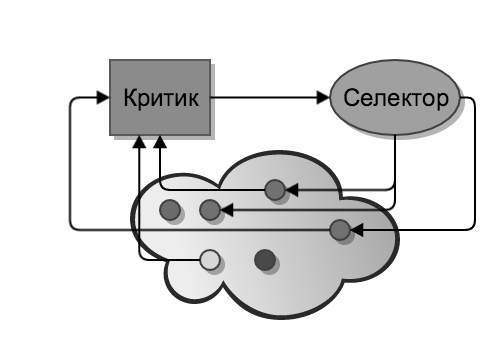
\includegraphics [scale=0.8] {csw_ex}
  \caption{\tripletshort\  в разрезе ресурсов} 
  \label{img:csw_ex}  
\end{figure}


\subsection{Основные компоненты модели}
\textbf{Уровни мышления}\par
Концепция уровней мышления представляет собой модель степени ментальной активности человека. Никто из людей не может похвастаться скоростью гепарда, гибкостью кошки или силой медведя. На наш взгляд, все это компенсируется возможностью изобретения образов мышления. Например, чтобы быть быстрыми, люди изобрели различные механизмы (самолеты, машины и др.). Чтобы быть сильными, они изобрели оружие. \par
 Все изобретения являются результатом взаимодействия человека с окружающим миром. Именно данное взаимодействие заставляет людей изобретать что-то новое, создавать шедевры литературы и летать в космос. По ходу своего развития разум человека проходит путь от врожденных инстинктов до возможности создания фундаментальных трудов, таких как  «Теории всего» \cite{Hawking}. В этом ему помогает возможность гибкого мышления: изобретение различных подходов к решению проблемы. Далее мы рассмотрим концепцию уровней мышления, следуя Марвину Мински \cite{EmotionMachine}. \par
Начнем с описания уровней мышления, которое представлено в таблице \ref{ThinkingLevelDescription}. Деление на данные уровни носит условный характер. Например, уровни 5 и 6 можно объединить, но, по словам Марвина Мински, принцип бритвы Оккама, который успешно применяется в физике, не должен также легко и однозначно применяться в психологии и теории мышления. \par




\begin{longtable}{|p{5cm}|p{11cm}|}
 \caption[Описание уровней мышления, предложенных Марвином Мински]{Описание уровней мышления, предложенных Марвином Мински}\label{ThinkingLevelDescription} \\ 
 \hline
 
 \multicolumn{1}{|c|}{\textbf{Уровень}} & \multicolumn{1}{c|}{\textbf{Описание}} \\ \hline 
\endfirsthead
\multicolumn{2}{c}%
{{\bfseries \tablename\ \thetable{} -- продолжение}} \\
\hline \multicolumn{1}{|c|}{\textbf{Уровень}} & \multicolumn{1}{c|}{\textbf{Описание}} \\ \hline 
\endhead

\endfoot

\hline \hline
\endlastfoot
Инстинктивный уровень & Происходят инстинктивные реакции (врожденные). Например, коленный рефлекс. Общую формулу для этого уровня можно выразить как «если ..., то сделать так». \\
  \hline

Уровень обученных реакций & Используются накопленные знания, то есть те знания, которым человек обучается в течение жизни. Например, переходить дорогу на зеленый свет. Общую формулу для этого уровня можно описать как «если ..., то сделать так». \\
  \hline

Уровень рассуждений & Мышление с использованием рассуждений. Например, если перебежать дорогу на зеленый свет, то можно успеть вовремя. На данном уровне сравниваются последствия нескольких решений и выбирается оптимальное. Общую формулу для этого уровня можно выразить как «если ..., то сделать так, тогда будет так». \\
  \hline

Рефлексивный уровень & Рассуждения с учетом анализа прошлых событий. Например, «в прошлый раз я побежал на моргающий зеленый и чуть не попал под машину». \\

  \hline
  Саморефлексивный уровень & Построение определенной модели, с помощью которой идет оценка своих поступков. Например, «мое решение не пойти на это собрание было неверным, так как я упустил столько возможностей, я был легкомысленным». \\
  \hline
  Самосознательный уровень & Оценка своих поступков с точки зрения высших идеалов и оценок окружающих. Например, «а что подумают мои друзья? А как бы поступил мой герой?» \\
  \hline

\end{longtable}


На рисунке \ref{img:thinkinglevels} представлено схематичное изображение уровней мышления, названных выше. 1--3 уровни составляют личность человека. 2--5 представляют ЭГО человека (Человеческое Я)~--- осознание человека в общении с окружающими. 3--6 представляют собой сверх ЭГО человека (сверх Я)~--- его моральные установки.
\begin{figure} [h] 
  \center
  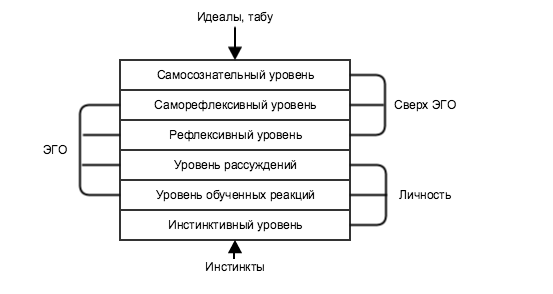
\includegraphics [scale=1.0] {thinkinglevels}
  \caption{Иллюстрация концепции Уровней мышления} 
  \label{img:thinkinglevels}  
\end{figure}


\textbf{Концепция k-line}. Эта концепция была первый раз упомянута Марвином Мински в 1987 году в журнале Cognitive Science. В книге \cite{SocietyOfMind} Марвин Мински раскрывает концепцию k-line. Полностью концепция описана позже в книге \cite{EmotionMachine}. 
K-line представляет собой связь между двумя событиями, объединяющими их в знание, например, объединение Образа мышления, найденного решения и активированной проблемы. 

На рисунке \ref{img:k_line} показана k-line, которая объединяет образы мышления, решения и других Критиков. Данная концепция позволяет «запоминать» удачные решения. 
\clearpage
\begin{figure} [h] 
  \center
  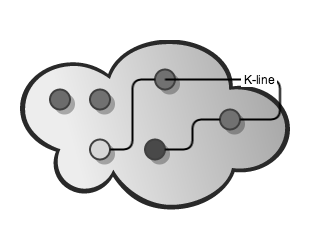
\includegraphics [scale=1.0] {k_line}
  \caption{Иллюстрация концепции k-line} 
  \label{img:k_line}  
\end{figure}
\section{Выводы по главе 2}
Модель Menta 0.1 имеет следующие недостатки: отсутствие устойчивости к грамматическим и содержательным ошибкам входной информации. Например, входной файл не имел отношения к программной системе, модель которой была в базе знаний в формате OWL; система поиска решения работала только в рамках модели одной программы; отсутствовала функция обучения. \par
В данный момент существует новый подход, который использует леса деревьев принятия решений \cite{DCFOREST}, он в рамках данной модели не рассматривался. Модель Menta 0.3 имеет следующие недостатки: отсутствие обучения; отсутствие обработки естественного языка; модуль HyperGraphDB оказался непригодным для промышленного использования; NARS в виду своих особенностей оказался непригодным для промышленного применения на значительном объеме фактов (>20), так как содержал в себе комбинаторный взрыв\footnote{Комбинаторный взрыв~--- термин, используемый для описания эффекта резкого («взрывного») роста временной сложности (до бесконечности) алгоритма при увеличении размера входных данных задачи.}. Например, при 10 фактах количество сочетаний будет равно 45 на первом уровне, далее алгоритм NARS будет сравнивать результаты этих сочетаний. Кроме того, после апробации оказалось, что критерии приемки практически описывают необходимое решение, что является недопустимым. Данный подход был описан в статье \cite{SoftwareAutomation}. \par

Для программной экспертной системы очень важно обладать способностью мыслить и рассуждать, например, очень важно для системы уметь проводить аналогии между уже известными разрешениями проблем и вновь появившимися. Множество запросов типично и отличается лишь параметрами. Например, пожалуйста, установите Office, Antivirus \etc\ \par
Также для экспертной системы важно уметь абстрагировать специализированные рецепты решения. К примеру, система научилась решать инцидент "Please install Firefox"\ («Пожалуйста, установите Firefox»). Абстрагировав данный инцидент до степени "Please install browser"\  («Пожалуйста, установите браузер»), система сможет теми же способами попробовать разрешить новую проблему.\par
После рассмотрения нескольких моделей была выбрана модель мышления Марвина Мински, так как она может быть адаптирована на области разрешения проблемных ситуаций, возникающих в процессе эксплуатации ИТ-инфраструктуры предприятия. На основе подхода Мински была построена модель системы, которая поддерживает основные функции: обучение, понимание инцидента, поиск решения, применение решения. 

\clearpage

           % Глава 2
\chapter{Реализация модели TU 1.0 для системы интеллектуальной регистрации и устранения проблемных ситуаций} \label{chapt3}
В данной главе рассматривается реализация модели TU: архитектура системы и программная реализация. Архитектура была создана с учетом принципов проектирования систем уровня Enterprise \cite{EA}.
\section{Архитектура системы} 
Данный раздел описывает основные режимы функционирования системы и концепцию ее построения. Архитектура системы представляет собой модульную систему, чтобы компоненты можно было удобно заменять \cite{M1}, например, подключать различные обработчики естественного языка. Основные компоненты системы описаны в таблице \ref{MainComponents}.
\begin{longtable}{|p{7cm}|p{9cm}|}
 \caption[Основные компоненты системы Thinking-Understanding (TU) ]{Основные компоненты системы Thinking-Understanding (TU) }\label{MainComponents} \\ 
 \hline
 
 \multicolumn{1}{|c|}{\textbf{Компонент}} & \multicolumn{1}{c|}{\textbf{Описание}}  \\ \hline 
\endfirsthead
\multicolumn{2}{c}%
{{\bfseries \tablename\ \thetable{} -- продолжение}} \\
\hline \multicolumn{1}{|c|}{\textbf{Компонент}} &
\multicolumn{1}{c|}{\textbf{Описание}}  \\ \hline 
\endhead

\endfoot

\hline \hline
\endlastfoot
\hline
   TU Webservice & Основной компонент взаимодействия с внешними система, включая пользователя \\
   \hline
   CoreService & Ядро системы, содержит основные классы\\
   \hline
   DataService & Компонент работы с данными \\
   \hline 
   Reasoner & Компонент вероятностной логики \\
   \hline 
   ClientAgent & Компонент выполнения скриптов на целевой машине \\
   \hline 
   MessageBus & Шина данных для системы \\

\end{longtable}

Система может работать в 2-х режимах: режим обучения и режим запроса. Диаграмма вариантов использования для режима обучения представлена на рисунке \ref{img:train}. Главным действующим лицом (согласно терминам UML) является специалист технической поддержки (TSS) (в общем случае это Пользователь (User)). Специалист технической поддержки может выполнять следующие действия: обучать систему; предоставлять правильное решение, если идет режим обучения; ввести запрос, если система функционирует в основном режиме; отслеживать применение исправления проблемы. 
Подробное описание представлено в таблице \ref{TrainUseCaseTable}. \par


\begin{longtable}{|p{7cm}|p{9cm}|}
 \caption[Описание ветвей в варианте использования «Режим обучения»]{Описание ветвей в варианте использования «Режим обучения»}\label{TrainUseCaseTable} \\ 
 \hline
 
 \multicolumn{1}{|c|}{\textbf{Ветвь}} & \multicolumn{1}{c|}{\textbf{Описание}}  \\ \hline 
\endfirsthead
\multicolumn{2}{c}%
{{\bfseries \tablename\ \thetable{} -- продолжение}} \\
\hline \multicolumn{1}{|c|}{\textbf{Ветвь}} &
\multicolumn{1}{c|}{\textbf{Описание}}  \\ \hline 
\endhead

\endfoot

\hline \hline
\endlastfoot
 \hline
communication:Train	& Обучение посредством коммуникации с системой специалиста технической поддержки \\
  \hline
communication:ProvidesSolution  & В случае коммуникации в режиме обучения специалист технической поддержки должен предоставить не только сам запрос, который будет формализован системой, но обучить систему алгоритму разрешения проблемы, содержащейся в запросе. Система формализует запрос, формализует решение и создаст между ними связи \\
  \hline
communication:ProvideRequest & Специалист технической поддержки вводит в систему запрос \\
  \hline
communication:MonitorsSolution  & Специалист технической поддержки смотрит, как применяется решение, если находится проблема, то решение корректируется посредством запроса CorrectSystemSolutions \\
  
\end{longtable}


\begin{figure} [h] 
  \center
  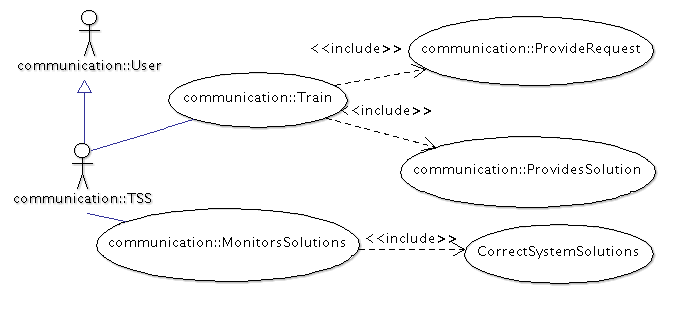
\includegraphics [scale=0.75] {UseCaseTrain}
  \caption{Вариант использования. Обучение} 
  \label{img:train}  
\end{figure}
Второй вариант использования~--- это основной поток. Главными действующим лицом системы является Заказчик (здесь и далее~--- Customer) (в общем случае это базовый класс Пользователь (здесь и далее~--- User)). Вариант использования имеет несколько ветвей, представленных в таблице \ref{ProductionUseCase}. В данном варианте система функционирует в «боевом режиме», то есть ищет ответ на запросы пользователя. В этом режиме есть возможность обучения: если система сталкнется с проблемой, то она задаст вопрос пользователю.
\begin{table} [htbp]
  \centering
  \parbox{15cm}{\caption{Описание ветвей в варианте использования «Основной режим»}\label{ProductionUseCase}}
%  \begin{center}
  \begin{tabular}{| p{10cm} | p{7cm} |}
 
  \hline
\textbf{Ветвь} & \textbf{Описание} \\
 
    \hline
ProvideRequest	& Заказчик вводит запрос в систему на естественном языке. Это могут быть либо прямая команда (например, Install Firefox, please), либо описание проблемы  \\
  \hline
communication:ProvideClarificationResponse  &  В случае, если система не может формализовать запрос либо нашлось множество решений, система запрашивает у пользователя детали
 \\
  \hline
communication:ProvideConfirmationResponse & В случае, когда система нашла решение, она запрашивает у пользователя подтверждение, что искомое решение решило его проблему
 \\

  \hline
  \end{tabular}
%  \end{center}
\end{table}
\clearpage
\subsection{Компоненты системы}
На рисунке \ref{img:MainComponentsCollaboration} представлено верхнеуровневое взаимодействие основных компонентов системы. В данном разделе будет дано краткое описание компонентов, последующие разделы будут посвящены отдельным компонентам, где будет представлено их подробное описание. В конце главы будет приведен подробный алгоритм взаимодействия всех компонентов системы.

\begin{figure} [h] 
  \center
  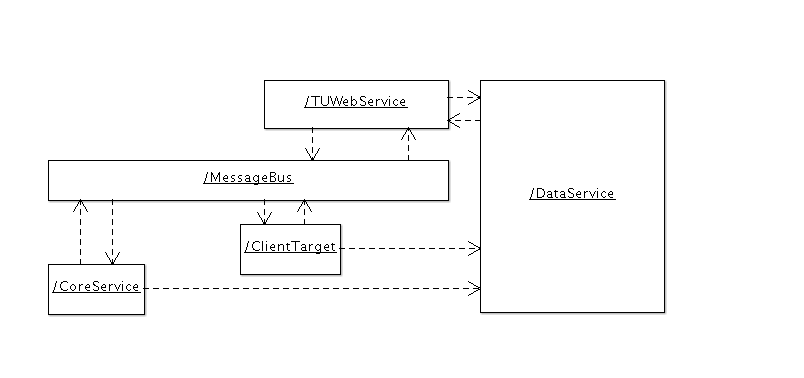
\includegraphics [scale=0.7] {MainComponentsCollaboration}
  \caption{Диаграмма взаимодействия компонентов} 
  \label{img:MainComponentsCollaboration}  
\end{figure}
Основной точкой взаимодействия (с позиции пользователя) с системой является компонент WebService (см. рисунок \ref{WebService}). Данный компонент построен на стандарте WS SOAP для универсального использования в различных внешних системах \cite{W1}. Взаимодействие происходит по следующей схеме:

\begin{enumerate}
	\item WebService получает запрос пользователя и сохраняет запрос в Базе Знаний (см. приложение \ref{Glossary});
	\item WebService отправляет сообщение типа Request с информацией о запросе в компонент MessageBus (шина);
	\item Один из экземпляров CoreService обрабатывает запрос;
	\item Компонент CoreService обрабатывает запрос и сохраняет результаты в Базе Знаний, затем он отправляет в MessageBus сообщение RequestCompleted и сообщение ActionsToExecute с указанием действий, которые необходимо исполнить;
	\item WebService получает сообщение RequestCompleted c результатами выполнения запроса и уведомляет подписчиков (конечных пользователей);
	\item Компонент ClientAgent получает сообщение ActionsToExecute со списком действий, которые необходимо исполнить на целевых машинах.
\end{enumerate} \par
Компонент MessageBus~--- это шина данных, которая обрабатывает сообщения и посылает их указанным компонентам. TUWebService~--- компонент взаимодействия с  «внешней средой», который предоставляет список функций и типов, посредством вызова которых можно обработать запрос в системе. Компонент DataService~--- отвечает за хранения данных, предоставляет базу заний для приложения. CoreService~--- ядро приложения, которое управляет основным жизненным циклом системы. ClientTarget~--- клиентский компонент для выполнения команд на машинах клиента. Сюда относятся как удаленное исполнение посредством WMI (Windows Management Instruments) и т.~п., так и непосредственная установка клиента на машины пользователей. На рисунке \ref{img:Component} (здесь и далее для детального изучения изображения, пожалуйста, воспользуйтесь функциями увеличения в pdf) представлено детальное описание компонентов с подкомпонентами. \par
Каждый верхнеуровневый компонент на рисунке \ref{img:Component} включает в себе более мелкие компоненты. Например, CoreService состоит из ThinkingLifeCycle~--- компонента управления жизненным циклом, Selector~--- компонента поиска и выбора ресурсов, Way2Think~--- компонента, описывающего алгоритмы поиска и применения решений и Critic~--- вероятностных триггеров, которые срабатывают на входящие события. Более детальное описание компонентов и механизмов представлено в остальных разделах данной главы. \par
В этой главе были представлены компоненты и их декомпозиция в разрезе системы. На рисунках видны крупноблочная структура системы, а также детальная~--- в разрезе общих блоков. Кроме того, описано взаимодействие с системой с точки зрения конечного пользователя, а также взаимодействия с другими системами. Также даны описание крупноблочных компонентов, а также детальное описание одного из основных компонентов.
\begin{figure} [h] 
  
  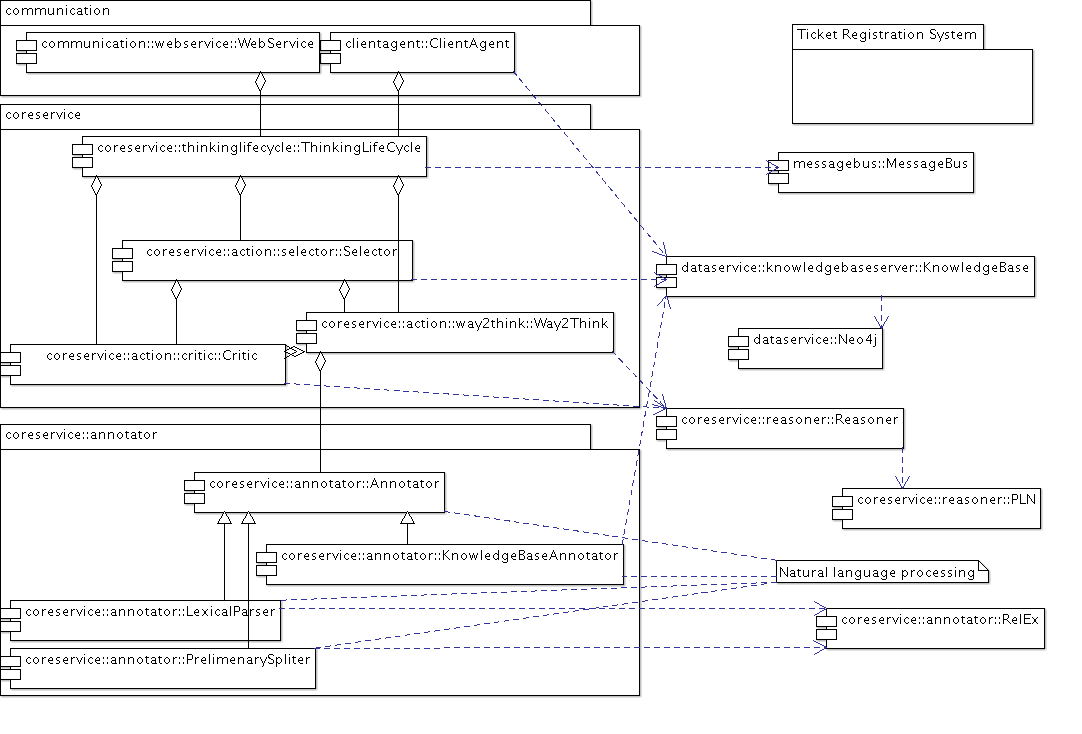
\includegraphics [scale=0.6, angle=90] {Component}
  \caption{Детальная диаграмма компонентов системы} 
  \label{img:Component}  
\end{figure}

\clearpage
\subsection{Компонент WebService} \label{WebService}
Данный компонент обрабатывает запросы пользователей, а также внешних систем. Запрос пользователя представляется посредством объекта Request, который содержит информацию о пользователя, а также ссылку на сервис пользователя, который будет вызван, когда запрос будет обработан. Вся работа происходит в компоненте CoreService.
На рисунке \ref{img:WebService} представлен интерфейс компонента.
В таблице \ref{WebServiceDescription} представлено описание методов.  
\begin{figure} [h] 
  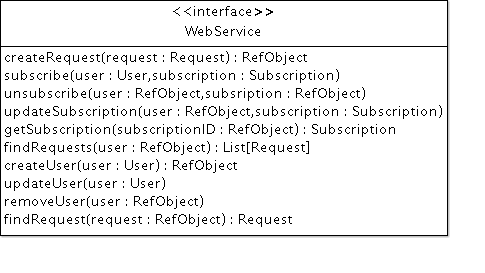
\includegraphics [width=0.8\textwidth,center] {WebService}
  \caption{Интерфейс компонента WebService} 
  \label{img:WebService}  
\end{figure}
Подробное описание классов представлено в приложении \ref{AppendixA}. Основной поток работы компонента состоит из следующих шагов:
\begin{enumerate}
	\item Пользователь создает запрос, используя метод WebService.createRequest;
	\item Система сохраняет запрос в Базе Знаний и начинает его обработку;
	\item Когда изменяется статус запроса (request.state), система оповещает подписчиков путем вызова ссылки на сервис пользователя, которая хранится в объекте Request.
\end{enumerate} \par
В общем виде данный компонент представляет фасад системы, ее внешнюю часть. Задача данного компонента~--- обеспечить легкое взаимодействие с системой и инкапсулировать основную логику системы. Соответствующие методы были подобраны так, чтобы внешним системам не нужно было реализовывать модель данной системы, а достаточно было использовать базовые облегченные объекты для приема и передачи информации. Данный подход подробно описан в книге Мартина Фаулера \cite{Patterns} и имеет название Data Transfer Object. В данном компоненте также широко используется подход Фасад, который также описан в названной книге. Архитектура компонента была проверена на предмет наличия антипаттернов проектирования, описанных в книге Вильяма Брауна \cite{AntiPatterns}. \par
В данном разделе был описан компонент взаимодействия с пользователям и внешними системами. Описаны архитектура компонента, основные методы, а также приведен пример основного потока.


\begin{table} [htbp]
   \center
   \parbox{15cm}{\caption{Описание методов компонента WebService}\label{WebServiceDescription}}
  \begin{tabular}{| p{8cm} |p{7cm} |}
  
  \hline
\textbf{Метод} & \textbf{Описание} \\
  \hline
  createRequest(request:Request): [RefObject] & Регистрирует запрос от пользователя. В качестве параметра в метод передается SubscriptionID, по которому идет проверка запроса \\
  
  \hline
  subscribe(user:User, subscription:Subscription)  & Создает подписку пользователя \\
  \hline
  unsubscribe(user:RefObject, subscription:RefObject)   & Убирает подписку пользователя \\
  \hline
  updateSubscription(user:RefObject, subscription:Subscription)   & Обновляет подписку пользователя \\
  \hline
  getSubscription(subscriptionID: RefObject): List<Request>    & Возвращает подписку \\
  \hline
  findRequests(user:RefObject)     & Возвращает запросы пользователя \\
  \hline
  createUser(user:User): RefObject     & Создает пользователя \\
  \hline
  updateUser(user:User)     & Обновляет информацию о пользователе \\ 
  \hline
  removeUser(user:RefObject)     & Удаляет информацию о пользователе \\ 
  \hline
  findRequest(request:RefObject): Request     & Возвращает запрос по ссылке \\ 
 
  \hline
\end{tabular}

\end{table}
\clearpage
\subsection{Компонент CoreService.ThinkingLifeCycle} \label{ThinkingLifeCycle}
Данный компонент системы отвечает за управление жизненным циклом системы: потоками, событиями приложения. Он запускает исполнение Критиков (Critic), Селекторов (Selector), Образов мышления (WayToThink), осуществляет обмен данных между компонентами. Компонент построен на фреймворке Akka Concurrency, который позволяет разрабатывать приложения, работающие параллельно \cite{AkkaConcurrency}. Архитектура модуля построена с учетом модели TU. \par
В данном компоненте реализовано шесть уровней мышления: Instinctive~--- инстинктивный уровень; Learned~--- уровень обученных реакций; Seliberative~--- уровень рассуждений; Reflective~--- рефлексивный уровень; Self-Reflective Thinking~--- саморефлексивный уровень; Self-Conscious Reflection~--- самосознательный уровень. \par

На уровне Instinctive идет обработка инцидентов, сгенерированных по шаблону.
Объект, который используется для обработки, применяет паттерн Akka \cite{AkkaConcurrency}. На рисунке \ref{img:ThinkingLifeCycle} представлена диаграмма классов компонента.  В таблице \ref{TLCCD} представлено подробное описание методов компонента с иллюстрациями. \par
На уровне Learned работают Критики классификации проблемы, они анализируют тип инцидента и активируют необходимые ресурсы. Более подробное описание работы Критиков приведено в следующих разделах. \par
На уровне Deliverative работает постановщик целей (который также является Критиком), который задает основные цели системы, тем самым запуская работу. Например, главная цель системы~--- решить проблему пользователя. Она активирует подцели, которые способствуют достижению основной цели. \par
На уровне Reflective работает Критик контроля времени, который отслеживает время выполнения запроса пользователя. \par
На уровне Self-Reflective Thinking осуществляется коммуникация с пользователем для уточнения запросов, проверки и применения найденного решения. \par
На уровне Self-Conscious работает Критик эмоционального состояния системы, который контролирует общее состояние системы и ее ресурсы. Критик контроля времени также обращается к этому критику для запроса ресурсов. \par
Данное расположение компонентов не случайно, оно реализует модель TU в привязке к различным уровням мышления. Проводя аналогию, можно сказать, что на более низких уровнях идет решение простых тактических задач, а на более высоких выстраивается общая стратегия поведения системы.
 
\begin{figure} [h] 
  \center
  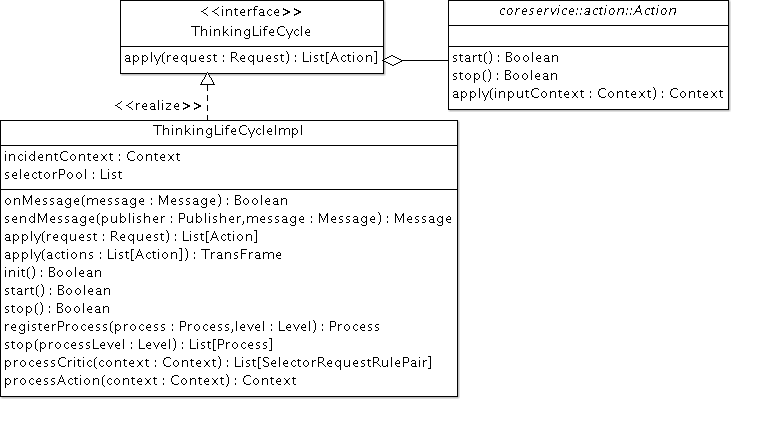
\includegraphics [scale=0.9,angle=90] {ThinkingLifeCycle}
  \caption{Диаграмма классов ThinkingLifeCycle} 
  \label{img:ThinkingLifeCycle}  
\end{figure}

\begin{longtable}{|p{7cm}|p{10cm}|}
 \caption[Описание методов класса (компонента) ThinkingLifeCycle]{Описание методов класса (компонента) ThinkingLifeCycle}\label{TLCCD} \\ 
 \hline
 
 \multicolumn{1}{|c|}{\textbf{Метод}} & \multicolumn{1}{c|}{\textbf{Описание}}  \\
\endfirsthead
\multicolumn{2}{c}%
{{\bfseries \tablename\ \thetable{} -- продолжение}} \\
\hline \multicolumn{1}{|c|}{\textbf{Метод}} &
\multicolumn{1}{c|}{\textbf{Описание}}  \\ \hline 
\endhead

\endfoot

\hline \hline
\endlastfoot
\hline
   onMessage(message : Message) & Данный метод вызывается при получении сообщения от шины. После этого происходит обработка запроса, формируется список действий, которые нужно выполнить. После этого запускается исполнение этих действий. На рисунке \ref{img:thinking-life-cycle-on-message-ad} представлена диаграмма действий этого метода \\
   \hline
   apply(request : Request) : List[Action] & Данный метод используется для запуска обработки входящего запроса. Для запроса создается контекст, если такой уже не был создан. После этого вызывается следующий компонент системы Selector, который выбирает необходимые ресурсы из Базы Знаний. На рисунке \ref{img:thinkinglifecycleapplyrequestRequestListAction} представлена диаграмма действий этого метода\\
   \hline
   apply(actions : List[Action]) : TransFrame & Данный метод запускает обработку действий. Все действия разделяются на Critic (триггеры действий, которые в итоге должны перейти в WayToThink через Selector) и WayToThink (образа мышления, непосредственые обработчики данных, классы, которые производят изменения данных). На рисунке \ref{img:thinkinglifecycleapplyactionsListActionTransFrame} представлена диаграмма действий этого метода \\
   \hline
   processWay2Think(inputContext: Context, outputContext: Context): TransFrame & Данный метод запускает обработку WayToThink. Он создает входной контекст (InputContext), заполняет его параметрами, создает выходной контекст OutputContext. Затем он запускает обработку данных во входном контексте. На рисунке \ref{img:thinkinglifecycleprocessWay2ThinkcontextContext} представлена диаграмма действий этого метода \\
    \hline
   processCritic(context: Context): List[SelectorRequestRulePair] & Данный метод запускает обработку Critic. На рисунке \ref{img:thinkinglifecycleactivityprocessCriticcontextContext} представлена диаграмма действий этого метода \\
   \hline
   init(): Boolean & Данный метод инициализирует экземпляр класса ThinkingLifeCycle. Во время инициализации происходят создание или подключение Базы Знаний (см. Словарь терминов \ref{Glossary}). На рисунке \ref{img:thinkinglifecycleinitBoolean} представлена диаграмма действий этого метода \\
    \hline
   start(): Boolean & Данный метод является необходимым для поддержки технологии Akka Concurrency, фактически он вызывает метод init \\
   \hline
   stop(): Boolean & Данный метод является необходимым для поддержки технологии Akka Concurrency, фактически он останавливает работу экземпляра класса: останавливается сессия к шине данных, останавливается подключение к Базе Знаний  \\
   \hline
   registerProcess(process : Process, level : Level) : Process & Данный метод ставит задачу в очередь исполнения. В качестве параметра принимается Level (уровень приоритета процесса) \\
   \hline
   stop(processLevel : Level) : List[Process] & Данный метод останавливает процесс. В качестве параметра принимается ссылка на процесс. На рисунке \ref{img:thinkinglifecyclestopprocessLevelLevelListProcess} представлена диаграмма действий этого метода  \\

 
 \hline 
\end{longtable}

\begin{figure} [h] 
  \center
  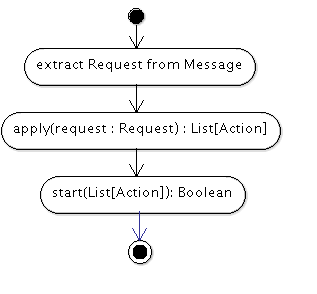
\includegraphics [scale=0.8] {thinkingLifeCycleonMessagemessageMessageBoolean}
  \caption{Диаграмма действий метода onMessage компонента ThinkingLifeCycle} 
  \label{img:thinking-life-cycle-on-message-ad}  
\end{figure}


\begin{figure} [h] 
  \center
  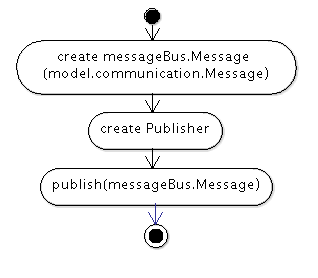
\includegraphics [scale=0.8] {thinkingLifeCyclesendMessagepublisherPublishermessageMessageMessage}
  \caption{Диаграмма действий метода sendMessage компонента ThinkingLifeCycle} 
  \label{img:thinking-life-cycle-send-message-publisher-publisher-ad}  
\end{figure}


\begin{figure} [h] 
  \center
  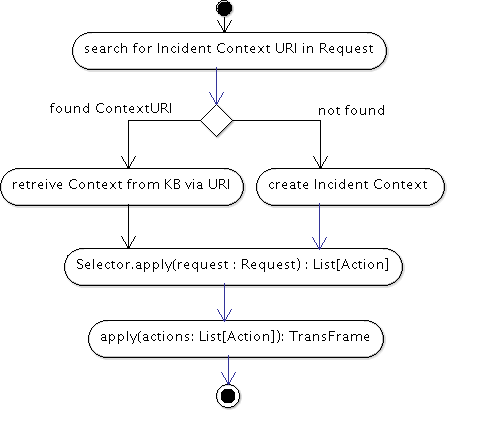
\includegraphics [scale=0.7] {thinkinglifecycleapplyrequestRequestListAction}
  \caption{Диаграмма действий метода apply компонента ThinkingLifeCycle} 
  \label{img:thinkinglifecycleapplyrequestRequestListAction}  
\end{figure}


\begin{figure} [h] 
  \center
  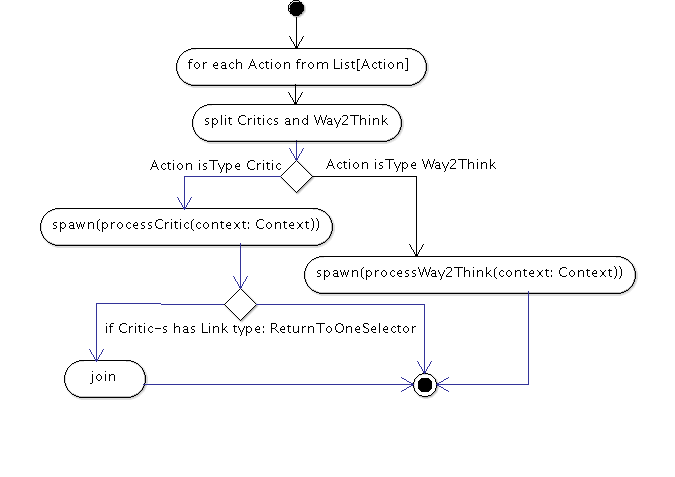
\includegraphics [scale=0.7] {thinkinglifecycleapplyactionsListActionTransFrame}
  \caption{Диаграмма действий метода apply компонента ThinkingLifeCycle} 
  \label{img:thinkinglifecycleapplyactionsListActionTransFrame}  
\end{figure}


\begin{figure} [h] 
  \center
  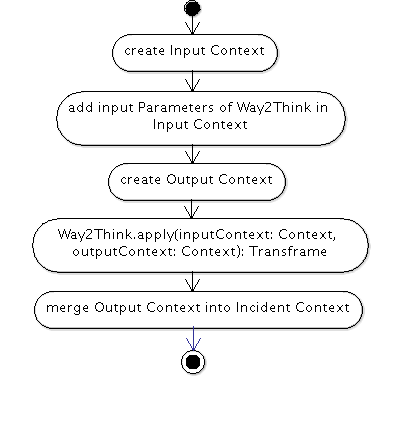
\includegraphics [scale=1.0] {thinkinglifecycleprocessWay2ThinkcontextContext}
  \caption{Диаграмма действий метода processWay2Think компонента ThinkingLifeCycle} 
  \label{img:thinkinglifecycleprocessWay2ThinkcontextContext}  
\end{figure}


\begin{figure} [h] 
  \center
  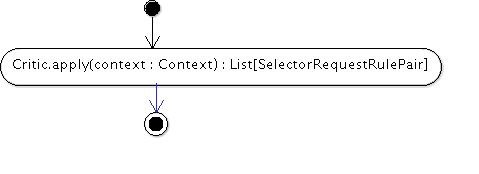
\includegraphics [scale=1.0] {thinkinglifecycleactivityprocessCriticcontextContext}
  \caption{Диаграмма действий метода processCritic компонента ThinkingLifeCycle} 
  \label{img:thinkinglifecycleactivityprocessCriticcontextContext}  
\end{figure}


\begin{figure} [h] 
  \center
  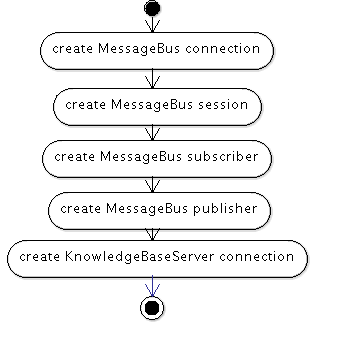
\includegraphics [scale=0.8] {thinkinglifecycleinitBoolean}
  \caption{Диаграмма действий метода init компонента ThinkingLifeCycle} 
  \label{img:thinkinglifecycleinitBoolean}  
\end{figure}

\begin{figure} [h] 
  \center
  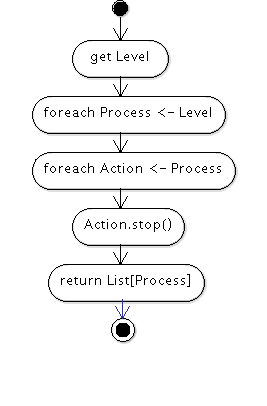
\includegraphics [scale=0.8] {thinkinglifecyclestopprocessLevelLevelListProcess}
  \caption{Диаграмма действий метода stop компонента ThinkingLifeCycle} 
  \label{img:thinkinglifecyclestopprocessLevelLevelListProcess}  
\end{figure}
\clearpage
\textbf{Описание работы компонента}. Чтобы понять работу компонента, далее рассмотрим описание алгоритма его работы. \par
\emph{Запуск и остановка}. Когда приложение запускается, оно инициализирует компонент ThinkingLifeCycle (далее TLC), который активирует набор критиков, базируясь на текущей цели системы. Например, если цель~--- классифицировать инцидент, то активируется набор критиков: разобрать, проверить, классифицировать. Когда приложение останавливается, оно останавливает все объекты класса и подклассов Actions (Critics, WayToThink), Selectors и ThinkingLifeCycle. \par
Коммуникация c остальными компонентами системы происходит посредством сообщений, отправленных через MessageBus (Шину Данных) JMS \cite{JMS}. Далее рассмотрим подробнее взаимодействие с остальными компонентами системы. \par
\begin{enumerate}
	\item Критик возвращает компоненту ThinkingLifeCycle (далее TLC) список Селекторов (SelectorRequestRule);
	\begin{enumerate}
	\item TLC запускает обработку компонента Selector;
	\item Selector возвращает TLC список Action (см. приложение \ref{AppendixB}) из Базы Знаний;
	\item TLC параллельно запускает возвращенные Action.
	\begin{enumerate}
	\item Если Action~--- это Critic;
	\item TLC создает InputContext (входной контекст приложения) и копирует туда все данные из Context (контекста) инцидента, созданного пользователем;
	\item Если Action~--- это Critic с ссылками ReturnToSameSelector, то TLC ждет результаты и отправляет компоненту Selector список SelectorRequestRule, которые были возвращены в качестве результата работы Critic. Иными словами, Critic может вернуть новый Selector. В данном случае нам нужно провести операцию Join для всех потоков \cite{JavaConcurrency}. В иных же случаях все Action запускаются в параллельных потоках.
	\end{enumerate} 
	\begin{enumerate}
	\item Если Action~--- это WayToThink;
	\item TLC создает InputContext (входной контекст приложения) и копирует туда все данные из Context (контекста), возвращенного Selector;
	\item TLC (см. таблицу \ref{Glossary}) запускает WayToThink;
	\item TLC сохраняет параметры в OutputContext;
	\item TLC сохраняет итоговый результат работы и возвращает его. 
	\end{enumerate} 
	\end{enumerate}
\end{enumerate} \par
В данном разделе было приведено описание основного цикла приложения с примерами работы. В следующих разделах содержится подробное описание работы каждого компонента на более низком уровне. В конце главы приведены развернутое описание стандартного цикла приложения и диаграмма расположения компонентов в разрезе уровней мышления.

%==============================
%==========Selector============
%==============================
\subsection{Компоненты \tripletshort} \label{Selector}\label{Critic}\label{WayToThink}
\textbf{Селектор (Selector)}~--- это компонент, который ответственен за получение списка действий и ресурсов из базы знаний, согласно входным параметрам. \par
\textbf{Входной критерий}. TLC запускает Selector c параметрами в виде контекста инцидента, который создал пользователь.  \par
\textbf{Выходной критерий}. Selector получает список Action: WayToThink или Critic. \par
\begin{figure} [h] 
  \center
  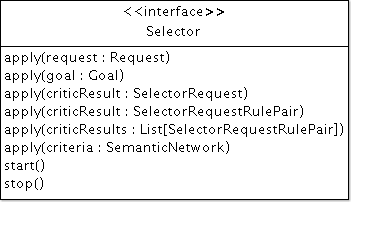
\includegraphics [scale=1.0] {SelectorInterface}
  \caption{Интерфейс компонента Selector} 
  \label{img:SelectorInterface}  
\end{figure} \par
На рисунке \ref{img:SelectorInterface} показан интерфейс компонент. В таблице \ref{SelectorMethodsDescription} приведено описание методов компонента.\\
\begin{longtable}{|p{7cm}|p{8cm}|}
 \caption[Описание методов класса (компонента) Selector]{Описание методов класса (компонента) Selector}\label{SelectorMethodsDescription} \\ 
 \hline
 
 \multicolumn{1}{|c|}{\textbf{Метод}} & \multicolumn{1}{c|}{\textbf{Описание}}  \\ \hline 
\endfirsthead
\multicolumn{2}{c}%
{{\bfseries \tablename\ \thetable{} -- продолжение}} \\
\hline \multicolumn{1}{|c|}{\textbf{Метод}} &
\multicolumn{1}{c|}{\textbf{Описание}}  \\ \hline 
\endhead

\endfoot

\hline \hline
\endlastfoot
\hline
  apply(request : Request) : Action & Данный метод на основе запроса пользователя получает из Базы знаний необходимые Critic \ref{Critic}. На рисунке \ref{img:applyrequestRequestActionActivity} представлена диаграмма действий этого метода \\
   \hline
   apply(goal: Goal) : Action & Данный метод на основе цели системы получает из Базы знаний необходимые Critic \ref{Critic}. На рисунке \ref{img:applygoalGoalActionActivity} представлена диаграмма действий этого метода\\
   \hline
   apply(criticResult : ActionProbabilityRule) : Action & Данный метод на основе работы Critic получает из Базы знаний необходимые Action. На рисунке \ref{img:applycriticResultActionProbabilityRulePairActionActivity} представлена диаграмма действий этого метода \\
 \hline 
\end{longtable}



\begin{figure} [h] 
  \center
  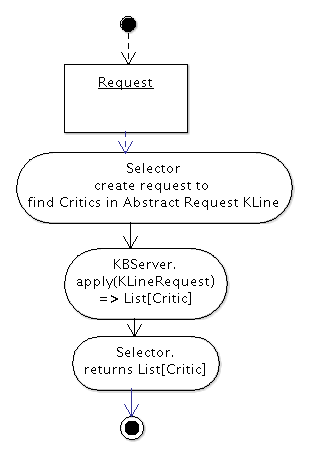
\includegraphics [scale=1.0] {applyrequestRequestActionActivity}
  \caption{Диаграмма действий метода Selector.apply(request : Request) компонента Selector} 
  \label{img:applyrequestRequestActionActivity}  
\end{figure}


\begin{figure} [h] 
  \center
  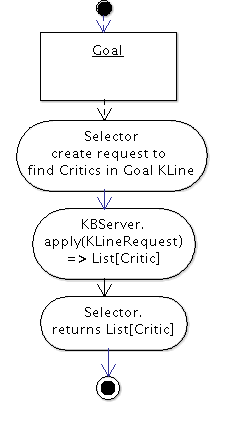
\includegraphics [scale=1.0] {applygoalGoalActionActivity}
  \caption{Диаграмма действий метода Selector.apply(goal: Goal) компонента Selector} 
  \label{img:applygoalGoalActionActivity}  
\end{figure}

\begin{figure} [h] 
  \center
  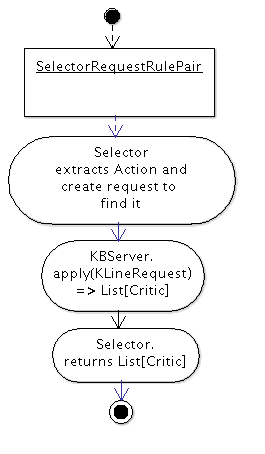
\includegraphics [scale=1.0] {applycriticResultActionProbabilityRulePairActionActivity}
  \caption{Диаграмма действий метода Selector.apply(criticResult : ActionProbabilityRule) компонента Selector} 
  \label{img:applycriticResultActionProbabilityRulePairActionActivity}  
\end{figure} \par



Чтобы лучше понять работу компонента и его назначение, далее рассмотрим сценарии его использования и взаимодействия с остальными компонентами на примере работы в режиме классификации входящего запроса.\par

\textbf{Действия при классификации входящего запроса} \par
\begin{enumerate}
	\item TLC (см. секцию \ref{ThinkingLifeCycle}) запускает входящие Critic (см. секцию \ref{Critic}) параллельно; 
	\item Когда Critic возвращает результат работы в виде ActionProbabilityRuleTriple, TLC запускает Selector с этим параметром;
	\item Selector запускает GetMostProbableWay2Think, который возвращает наиболее вероятный WayToThink;
	\item В некоторых случаях Selector может вернуть менее вероятный вариант, если на уровне мышления Reflective после проверки решения, оно было признано некорректным, или же пользователь признал его таким.
\end{enumerate} \par
На рисунке \ref{img:classifyIncidentActivity} представлена диаграмма действий классификации инцидента. TLC (см. секцию \ref{ThinkingLifeCycle}) получает цель классифицировать инцидент, затем Selector по этой цели возвращает Critic. После чего TLC запускает обработку Critic в разных потоках (параллельно). В данном случае рассматривается три Critic: DirectInstruction~--- прямые инструкции, данный Critic возвращает WayToThink Simulate (см. секцию \ref{WayToThink}), который ищет связь между концепциями в запросе и концепциями в Базе Знаний; ProblemWithDesiredState~--- проблема с ожидаемым результатом, данный Critic возвращает Simulate и Reformulate WayToThink, которые ищут сопоставление концепциями в Базе Знаний и пытается преобразовать запрос к DirectInstruction запросу (прямым инструкциям); ProblemWithoutDesiredState~--- проблема без ожидаемого результата, данный Critic возвращает Simulate, Reformulate, InferDesiredState, который пытается преобразовать проблему к ProblemWithDesiredState. \par
После работы компонента TLC (см. секцию \ref{ThinkingLifeCycle}) собирает результаты выполнения всех Critic и запускает их, пока не будет достигнута изначальная цель. \par
\begin{figure} [h] 
  \center
  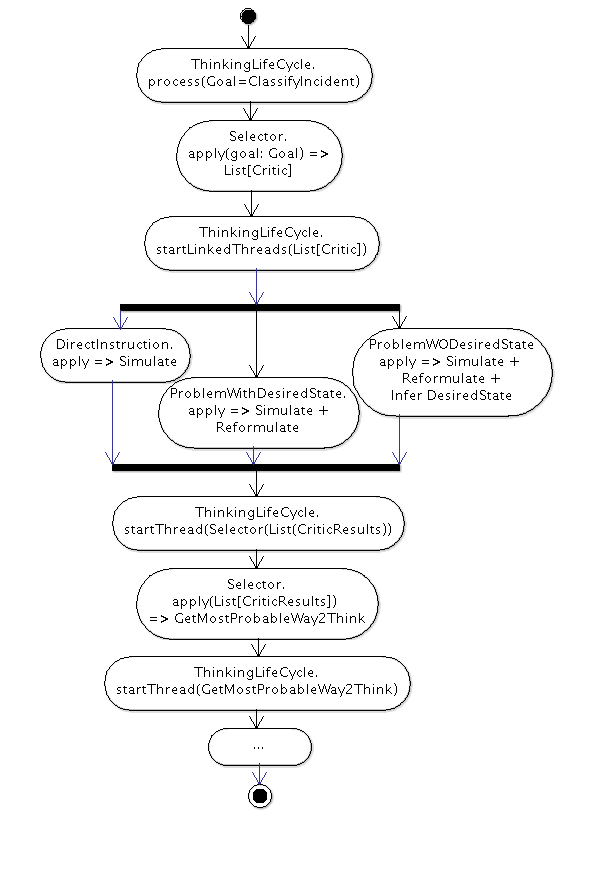
\includegraphics [scale=0.8] {classifyIncidentActivity}
  \caption{Диаграмма действий классификации инцидента} 
  \label{img:classifyIncidentActivity}  
\end{figure}
В данном разделе была описана работа компонента Selector с примерами работы и демонстрацией интеграции с остальными компонентами. Данный компонент тесно связан с компонентом TLC \ref{ThinkingLifeCycle}. Особенностью работы компонента является то, что список ресурсов, который он возвращает, можно задавать динамически, он также может формироваться во время работы системы. \par
\clearpage
%============================================
%===============Critic=======================
%============================================
\textbf{Critic} является основным компонентом для анализа в \tripletshort. Critic используется для классификации входной информации, рефлексии, само-анализа и служит определенным вероятностным переключатетелем. Например, компоненты контроля времени, контроля эмоционального состояния системы~--- это тоже Critic. \par
\textbf{Входной критерий}. TLC \ref{ThinkingLifeCycle} запускает Critic согласно Goal (Цель) (см. Приложение \ref{AppendixB}) или входящему запросу от пользователя. \par
\textbf{Выходной критерий}. Critic генерирует SelectorRequest \ref{Selector}. 
На входе Critic принимает: загруженные из базы правила для работы Critic (CriticRules); DomainModel:SemanticNetwork (см. \ref{acronyms})~--- доменная модель, представляющая собой семантическую сеть; описание инцидента, представляющее собой семантическую сеть. \par
На выходе Critic предоставляет: SelectorRequest \ref{Selector}~--- запрос на выбор Selector из базы знаний; CriticRule~--- правило, которое сработало для активации. Данное правило является логическим предикатом, т.~е. содержит в себе определенную формулу для вычисления вероятности. \par
На рисунке \ref{img:CriticApply} представлена диаграмма действий Critic, описание диаграммы приведено в таблице \ref{CriticMethods}.  В системе существуют разные типы Critic, их описание доступно в таблице \ref{CriticTypesRaw}.
\begin{figure} [h] 
  \center
  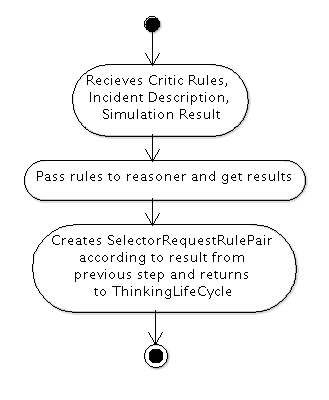
\includegraphics [scale=1.0] {CriticApply}
  \caption{Диаграмма действий компонента Critic} 
  \label{img:CriticApply}  
\end{figure}

\begin{longtable}{|p{7cm}|p{10cm}|}
 \caption[Описание основных типов Critic, используемых в системе]{Описание основных типов Critic, используемых в системе}\label{CriticTypesRaw} \\ 
 \hline
 
 \multicolumn{1}{|c|}{\textbf{Critic}} & \multicolumn{1}{c|}{\textbf{Описание}}  \\ \hline 
\endfirsthead
\multicolumn{2}{c}%
{{\bfseries \tablename\ \thetable{} -- продолжение}} \\
\hline \multicolumn{1}{|c|}{\textbf{Critic}} &
\multicolumn{1}{c|}{\textbf{Описание}}  \\ \hline 
\endhead

\endfoot

\hline \hline
\endlastfoot
\hline
   Manager & простой тип критика, который работает как триггер, например, Goal (см. приложение \ref{AppendixB}), который запускает необходимый WayToThink \\
   \hline
   Control & контролирующий Critic, который ждет определенного события (срабатывает на определенное событие). Например, заканчивается отведенное на решение время\\
   \hline
   Analyser & анализатор, обрабатывает и выявляет тип инцидента. Например, прямые инструкции, проблема с желаемым состоянием, выбор наиболее вероятного действия \\
 \hline 
\end{longtable}

\begin{longtable}{|p{8cm}|p{9cm}|}
 \caption[Описание методов компонента Critic]{Описание методов компонента Critic}\label{CriticMethods} \\ 
 \hline
 
 \multicolumn{1}{|c|}{\textbf{Метод}} & \multicolumn{1}{c|}{\textbf{Описание}}  \\ \hline 
\endfirsthead
\multicolumn{2}{c}%
{{\bfseries \tablename\ \thetable{} -- продолжение}} \\
\hline \multicolumn{1}{|c|}{\textbf{Метод}} &
\multicolumn{1}{c|}{\textbf{Описание}}  \\ \hline 
\endhead

\endfoot

\hline \hline
\endlastfoot
\hline
   exclude():List[CriticLink] & Данный метод возвращает список CriticLink, которые при срабатывание данного Critic будут игнорироваться с определенной вероятностью, после срабатывания Critic будет посчитана суммарная вероятность активации. После чего система решит, какой Critic был вероятнее всего активирован. \\
   \hline
   include():List[Critic] & Данный метод возвращает список объектов класса CriticLink, которые при срабатывание данного Critic будут включаться с определенной вероятностью.\\
   \hline
   apply(currentSituation: SemanticNetwork, domainModel:SemanticNetwork): List[SelectorRequestRulePair] & Данный метод запускает Critic, после чего вернется список Selector (см. секцию \ref{Selector}) с определенной веротяностью, после чего TLC (см. секцию \ref{ThinkingLifeCycle}) их активирует. \\
 \hline 
\end{longtable} 
Как сказано выше, Critic действуют на разных уровнях мышления. Далее приведено описание Critic с привязкой к уровням мышления.
\begin{enumerate}
	\item Уровень обученных реакций;
	\begin{enumerate}
		\item PreprocessManager~--- предобработка информации;
		\item Классификаторы инцидентов: Прямые инструкции, Проблема с желаемым состоянием, Проблема без желаемого состояния;
		\item SolutionCompletenessManager~--- связывается с пользователем и проверяет устраивает ли его найденное решение.
	\end{enumerate}
	\item Уровень рассуждений;
	\begin{enumerate}
		\item Выбор наиболее вероятного Selector по Rule. Данный Critic после проверки правил, выбирает из них правило с большей вероятностью.
	\end{enumerate}
	\item Рефлексивный уровень;
	\begin{enumerate}
		\item Менеджер целей. Установка целей.
	\end{enumerate}
	\item Саморефлексивный уровень;
	\begin{enumerate}
		\item ProcessingManager~--- запускает выполнение запроса;
		\item TimeControl~--- контроль времени исполнения запроса;
		\item DoNotUnderstandManager~--- активируется, когда необходимо уточнение пользователя для продолжения работы.
	\end{enumerate}
	\item Самосознательный уровень.
	\begin{enumerate}
		\item EmotionalStateManager~--- контроль общего состояния системы.
	\end{enumerate} 
\end{enumerate} \par
Основным примером работы компонента может служить классификация инцидентов (подробнее рассматривалось ранее). Например, у нас есть Critic для прямых инструкций DirectInstruction, есть для ситуации с желаемым состоянием DesiredState. Пусть на входе будет запрос вида: install antivirus. DesiredState найдет здесь действие~--- install, но не найдет желаемого состояния, то есть вероятность его выполнения будет 60\%. DirectInstruction будет искать действие и объект, которые присутствуют в запросе, его вероятность будет 100\%, его TLC (см. секцию \ref{ThinkingLifeCycle}) и активируют как наиболее вероятный. \par
Это был простой пример работы компонента, на самом деле механизм работы гораздо гибче: он поддерживает включения, исключения, составные правила и логику. Компонент также является динамически формируемым. \par
В данном разделе был описан важный компонент системы, который определяет алгоритм ее работы, в этом компоненте скрыта основная возможность системы думать и решать, согласно набором правил и внешним обстоятельствам. \par

%=================================
%===========WayToThink============
%=================================
\textbf{WayToThink} является основным операционным компонентом \tripletshort. Основными задачами данного компонента являются: обновление, преобразование, сохранение данных и коммуникация с пользователем, иными словами, все, что в той или иной форме изменяет операционный контекст данных системы. \par
\textbf{Входной критерий}. Запуск осуществляется из компонента ThinkingLufeCycle (см. секцию \ref{ThinkingLifeCycle}). Входными данными является InputContext, который содержит параметры WayToThink.\par
\textbf{Выходной критерий}. WayToThink завершил работу. На выходе возвращают измененные в ходе работы данные. В общем виде компонент описывает последовательность действий. В системе используется два больших класса WaytToThink~--- простой и составной (сложный). Простые WayToThink являются встроенными в систему, остальные являются комбинацией компонентов: Critic \ref{Critic}, Selector \ref{Selector}, WayToThink \ref{WayToThink}. В таблице \ref{WayToThinkList} приведено описание встроенных в систему WayToThink. На рисунке \ref{img:Way2ThinkInterface} представлен интерфейс компонента. В таблице \ref{WayToThinkMethods} представлено описание методов WayToThink.  

\begin{figure} [h] 
  \center
  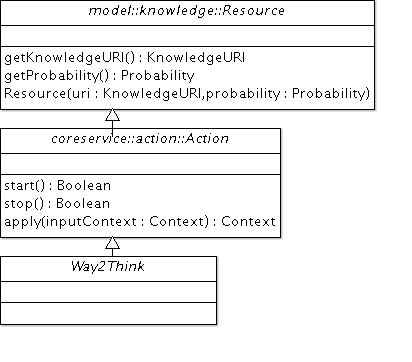
\includegraphics [scale=0.8] {Way2ThinkInterface}
  \caption{Интерфейс компонента WayToThink} 
  \label{img:Way2ThinkInterface}  
\end{figure}

\begin{longtable}{|p{7cm}|p{10cm}|}
 \caption[Описание встроенных в систему WayToThink]{Описание встроенных в систему WayToThink}\label{WayToThinkList} \\ 
 \hline
 
 \multicolumn{1}{|c|}{\textbf{WayToThink}} & \multicolumn{1}{c|}{\textbf{Описание}}  \\ \hline 
\endfirsthead
\multicolumn{2}{c}%
{{\bfseries \tablename\ \thetable{} -- продолжение}} \\
\hline \multicolumn{1}{|c|}{\textbf{WayToThink}} &
\multicolumn{1}{c|}{\textbf{Описание}}  \\ \hline 
\endhead

\endfoot

\hline \hline
\endlastfoot
\hline
   Создать контекст & Данный WayToThink создает объект Context для аккумуляции данных запроса \\
   \hline
   Установить общий статус системы & Данный WayToThink устанавливает состояние системы в глобальном контексте\\
   \hline
   Установить цель системы & Данный WayToThink устанавливает цель запроса в текущем контексте  \ref{AppendixB} \\
    \hline
   Разделить фразу на слова и предложения & Данный WayToThink разбивает фразу на слова и возвращает список слов\\
    \hline
   Найти связи между входной информацией и базой знаний & Данный WayToThink ищет связь между входной информацией и базой знаний\\ 
   \hline
   Извлечь связи & Данный WayToThink возвращает список связей из фразы\\
    \hline
   Сохранить наиболее вероятное решение & Данный WayToThink сохраняет наиболее вероятное решение\\
    \hline
   Перефразировать (Reformulate) & Данный WayToThink ищет связь между текущим контекстом и известными проблемами, если есть неизвестные концепции, то он пытается их переформулировать при помощи пользотеля\\
   \hline
   Смоделировать (Simulate) & Данный WayToThink ищет связь между текущим контекстом и проблемами уже сохраненными в базе\\
   \hline
   Найти решение & Данный WayToThink производит поиск решения, которое прикреплено к проблеме, которая была найдена при помощи моделирования и перефразирования\\
   \hline
   Остановить работу & Данный WayToThink останавливает работу системы\\
 \hline 
\end{longtable}

\begin{longtable}{|p{7cm}|p{10cm}|}
 \caption[Описание методов компонента WayToThink]{Описание методов компонента WayToThink}\label{WayToThinkMethods} \\ 
 \hline
 
 \multicolumn{1}{|c|}{\textbf{Метод}} & \multicolumn{1}{c|}{\textbf{Описание}}  \\ \hline 
\endfirsthead
\multicolumn{2}{c}%
{{\bfseries \tablename\ \thetable{} -- продолжение}} \\
\hline \multicolumn{1}{|c|}{\textbf{Метод}} &
\multicolumn{1}{c|}{\textbf{Описание}}  \\ \hline 
\endhead


\endfoot

\hline \hline
\endlastfoot
\hline
   start() & Запустить обработку информации \\
   \hline
   stop() & Остановить обработку, например, если выполнение идет слишком долго\\
   \hline
   apply(inputContext:Context): Context & Применить WayToThink. Исполнение начнется только после вызова метода start \\
    \hline
\end{longtable}

WayToThink также используется как описание алгоритма разрешения проблемы (см. приложение \ref{AppendixDHowTo} HowTo), то есть описывает последовательность действий, необходимых для устранения проблемной ситуации. \par
В зависимости от типа WayToThink активируется та или иная последовательность действий. В общем виде последовательность имеет следующий вид: получить данные, обработать, вернуть данные. В случае, например, WayToThink Simulate второй шаг имеет вид «найти связь между текущим контекстом и проблемами, уже сохраненными в Базе Знаний». Если же WayToThink является описанием решения, то второй шаг может быть набором вызова системных утилит с параметрами из первого шага. \par
В данном разделе был описан основной компонент модификации данных WayToThink. Нужно отметить, что данный компонент также является важной частью модели TU. Проектировался он для универсального применения во всех случаях, когда необходимо действие над данными. Например, если нужно использовать скрипт, который был написан на языке интерпретации Bash, и ввести его в систему, можно разбить каждый шаг и вызов на отдельную часть и сделать сложный WayToThink с ветвлениями и циклами. \par
\begin{figure} [h] 
  \center
  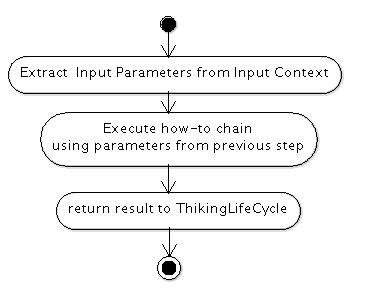
\includegraphics [scale=0.8] {way2thinkHowToActivity}
  \caption{Работа компонента WayToThink в режиме описания решения проблемы (HowTo) } 
  \label{img:way2thinkHowToActivity}  
\end{figure}
%===================================
%===========PreliminaryAnnotator====
%===================================
\clearpage
\subsection{Вспомогательные компоненты} \label{PreliminaryAnnotator}\label{KnowledgeBaseAnnotator}\label{data service}\label{Reasoner}
Данный компонент проводит предварительную подготовку текста: грамматическую и орфографическую коррекции текста, а также разделение на предложения. На рисунке \ref{img:PrelimenaryAnnotatorInterface} представлен интерфейс компонента. Компонент также является WayToThink, так как он производит модификацию данных контекста. В таблице \ref{PrelimenaryAnnotatorMethods} приведено описание методов класса.
\begin{figure} [h] 
  \center
  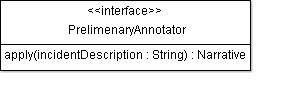
\includegraphics [scale=1.0] {PrelimenaryAnnotatorInterface}
  \caption{Интерфейс компонента PrelimenaryAnnotator} 
  \label{img:PrelimenaryAnnotatorInterface}  
\end{figure}
\begin{longtable}{|p{7cm}|p{10cm}|}
 \caption[Описание методов компонента PrelimenaryAnnotator]{Описание методов компонента PrelimenaryAnnotator}\label{PrelimenaryAnnotatorMethods} \\ 
 \hline
 
 \multicolumn{1}{|c|}{\textbf{Метод}} & \multicolumn{1}{c|}{\textbf{Описание}}  \\ \hline 
\endfirsthead
\multicolumn{2}{c}%
{{\bfseries \tablename\ \thetable{} -- продолжение}} \\
\hline \multicolumn{1}{|c|}{\textbf{Метод}} &
\multicolumn{1}{c|}{\textbf{Описание}}  \\ \hline 
\endhead


\endfoot

\hline \hline
\endlastfoot
\hline
   apply(incidentDescription:String): Narrative & Данный метод запускает обработку входного текста и его корректировку \\
   \hline
  \end{longtable}
С точки зрения корректировки текст подвергается обработке средствами проверки языка, например, открытый комплекс After the deadline \cite{AfterTheDeadline}, а также Google API. В части разбиения текста на слова используется алгоритм из открытого комплекса Link Grammar \cite{LG-2}. В целом компонент содержит в себе также составную системы разбора, что отличает его от прямого использования алгоритма. Он манипулирует результатом работы из нескольких подсистем, для увеличения степени точности. \par
Одной из особенностью компонента является использование внутренней базы знаний для предобработки текста, чтобы убрать неточности, которые будут мешать работе средств NLP. Например, часто средства NLP не понимают концепцию слова please, поэтому в базе изначально хранится эта концепция с правильным значением. Таким образом, на вход средствам NLP поступает уже аннотированный текст, что позволяет на 20\% (согласно экспериментальным данным) увеличить точность обработки. \par
%===================================
%===========KnowledgeBaseAnnotator==
%===================================
\textbf{Компонент CoreService.KnowledgeBaseAnnotator}\par 
Данный компонент устанавливает связи между терминами во входной фразе и базой знаний и также является WayToThink \ref{WayToThink}.  \par
\textbf{Входные критерии}. Список подготовленных фраз в виде объектов. \par
\textbf{Выходные критерии}. Список ссылок на внутренние знания. \par
\textbf{Описание работы компонента} \par
\begin{enumerate}
	\item Получен Термин;
	\item Поиск в локальной базе знаний;
	\item Если совпадение не найдено идет запрос во внешнюю базу знаний;
	\item Внешняя база возвращает список синонимов;
	\item Компонент ищет по синонимам во внутренний базе знаний;
	\item Если поиск успешен, то создается связь между входящем термином, синонимом и концепцией в базе знаний.
\end{enumerate}
Например, входящий запрос содержит термин "program"\,, база знаний содержит термин "computer software". Идет запрос во внешние базы знаний, найдено "computer software, program". Будет добавлена связь-аналогия в база знаний "program~--- computer software". 


%===================================
%===========DataService==
%===================================
\textbf{Компонент DataService} \par
Данный компонент отвечает за хранение данных в системе. База знаний построена на графах. На рисунке \ref{img:KnowledgeBaseServer} представлен интерфейс компонента. В базе знаний используется два типа объектов Object~--- объект базы знаний, BusiessObject~--- объект для Web Service (User, Request). BusinessObject является кортежем для интеграции с внешними системами. У объекта есть ID, который уникально удостоверяет его в рамках системы. В таблице \ref{DataServiceMethods} приведено описание методов компонента. \par
\begin{figure} [h] 
  \center
  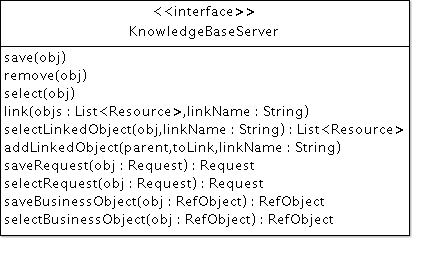
\includegraphics [scale=0.8] {KnowledgeBaseServer}
  \caption{Интерфейс компонента KnowledgeBaseServer} 
  \label{img:KnowledgeBaseServer}  
\end{figure}
\begin{longtable}{|p{8cm}|p{9cm}|}
 \caption[Описание методов компонента DataService]{Описание методов компонента DataService}\label{DataServiceMethods} \\ 
 \hline
 
 \multicolumn{1}{|c|}{\textbf{Метод}} & \multicolumn{1}{c|}{\textbf{Описание}}  \\ \hline 
\endfirsthead
\multicolumn{2}{c}%
{{\bfseries \tablename\ \thetable{} -- продолжение}} \\
\hline \multicolumn{1}{|c|}{\textbf{Метод}} &
\multicolumn{1}{c|}{\textbf{Описание}}  \\ \hline 
\endhead


\endfoot

\hline \hline
\endlastfoot
\hline
   save(obj:Resource): Resource  & Данный метод позволяет сохранить ресурс в базу знаний \\
   \hline
   remove(obj:Resource)  & Данный метод позволяет удалить объект \\
   \hline
   select(obj:Resource): Resource  & Данный метод позволяет выбрать объект \\
   \hline
   link(obj:List<Resource>, linkName:String)  & Данный метод позволяет сделать ссылку между 2-мя объектами \\
   \hline
   selectLinkedObject(obj:Resource, linkName:String): Link<Resource>  & Данный метод позволяет выбрать все объекты, которые имеют связь под названием linkName с объектом obj \\
   \hline
   addLinkedObject(parent:Resource, toLink:Resource, linkName:String)  & Данный метод позволяет создать ссылку linkName с объектом \\
   \hline
   saveRequest(obj:Request)  & Данный метод позволяет получить запрос из Базы Знаний \\
   \hline
   selectRequest(obj:RefObject)  & Данный метод позволяет получить запрос из Базы Знаний \\
   \hline
   saveBusinessObject(obj:RefObject): RefObject  & Данный метод позволяет сохранить объект в базу \\
   \hline
   selectBusinessObject(obj:RefObject): RefObject  & Данный метод позволяет полуить объект из Базы Знаний \\
   \hline
  \end{longtable}

%=================================
%===========Reasoner===========
%=================================
\textbf{Компонент Reasoner} \par
Данный компонент осуществляет логические вычисления для системы, например, для обработки правил в компоненте Critic \ref{Critic}. На рисунке \ref{img:ReasonerInterface} представлен интерфейс компонента. В таблице \ref{ReasonerMethods} приведено описание методов компонента. 
%ReasonerInterface.png 
\begin{figure} [h] 
  \center
  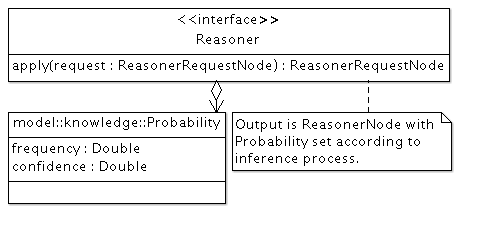
\includegraphics [scale=0.8] {ReasonerInterface}
  \caption{Интерфейс компонента Reasoner} 
  \label{img:ReasonerInterface}  
\end{figure}
\begin{longtable}{|p{7cm}|p{10cm}|}
 \caption[Описание методов компонента Reasoner]{Описание методов компонента Reasoner}\label{ReasonerMethods} \\ 
 \hline
 
 \multicolumn{1}{|c|}{\textbf{Метод}} & \multicolumn{1}{c|}{\textbf{Описание}}  \\ \hline 
\endfirsthead
\multicolumn{2}{c}%
{{\bfseries \tablename\ \thetable{} -- продолжение}} \\
\hline \multicolumn{1}{|c|}{\textbf{Метод}} &
\multicolumn{1}{c|}{\textbf{Описание}}  \\ \hline 
\endhead

\endfoot

\hline \hline
\endlastfoot
\hline
   apply(request: ReasonerRequestNode): ReasonerRequestNode  & Данный метод проводит обработку правил и считает вероятность (Probability) и уверенность (Confidence) \\
   \hline
  
  \end{longtable}
На данный момент времени в качестве реализации в системе используется два движка логический вычисление PLN \cite{PLN} и NARS \cite{NARS}. Основным применением данного компонента являются правила для Critic. Логика правил обрабатывается при помощи этого компонента. Этот результат используется для определения вероятности активации данного Critic. Подобное использование дает гибкость в построении свода правил. 
  
\clearpage
%=================================
%===========Knowledge=============
%=================================
\section{Модель данных TU Knowledge} 
Одной из важных частей системы является реализация хранения данных на основе модели TU. Для работы системы была разработана уникальная схема данных~--- TU Knowledge, которая сочетает в себе OWL и графовую базу данных. Язык OWL, традиционно использующийся для структурирования информации в Вебе \cite{OWL}, обрел широкое использование во многих схемах данных, так как давал возможность дополнительного расширенного описания взаимосвязи между данными. На рисунке \ref{img:KnowledgeClass} представлена схема данных TU Knowledge. В таблице \ref{TUKnowledge} представлено описание схемы TU Knowledge.
%\begin{landscape}
\begin{figure} [h] 
  \center
  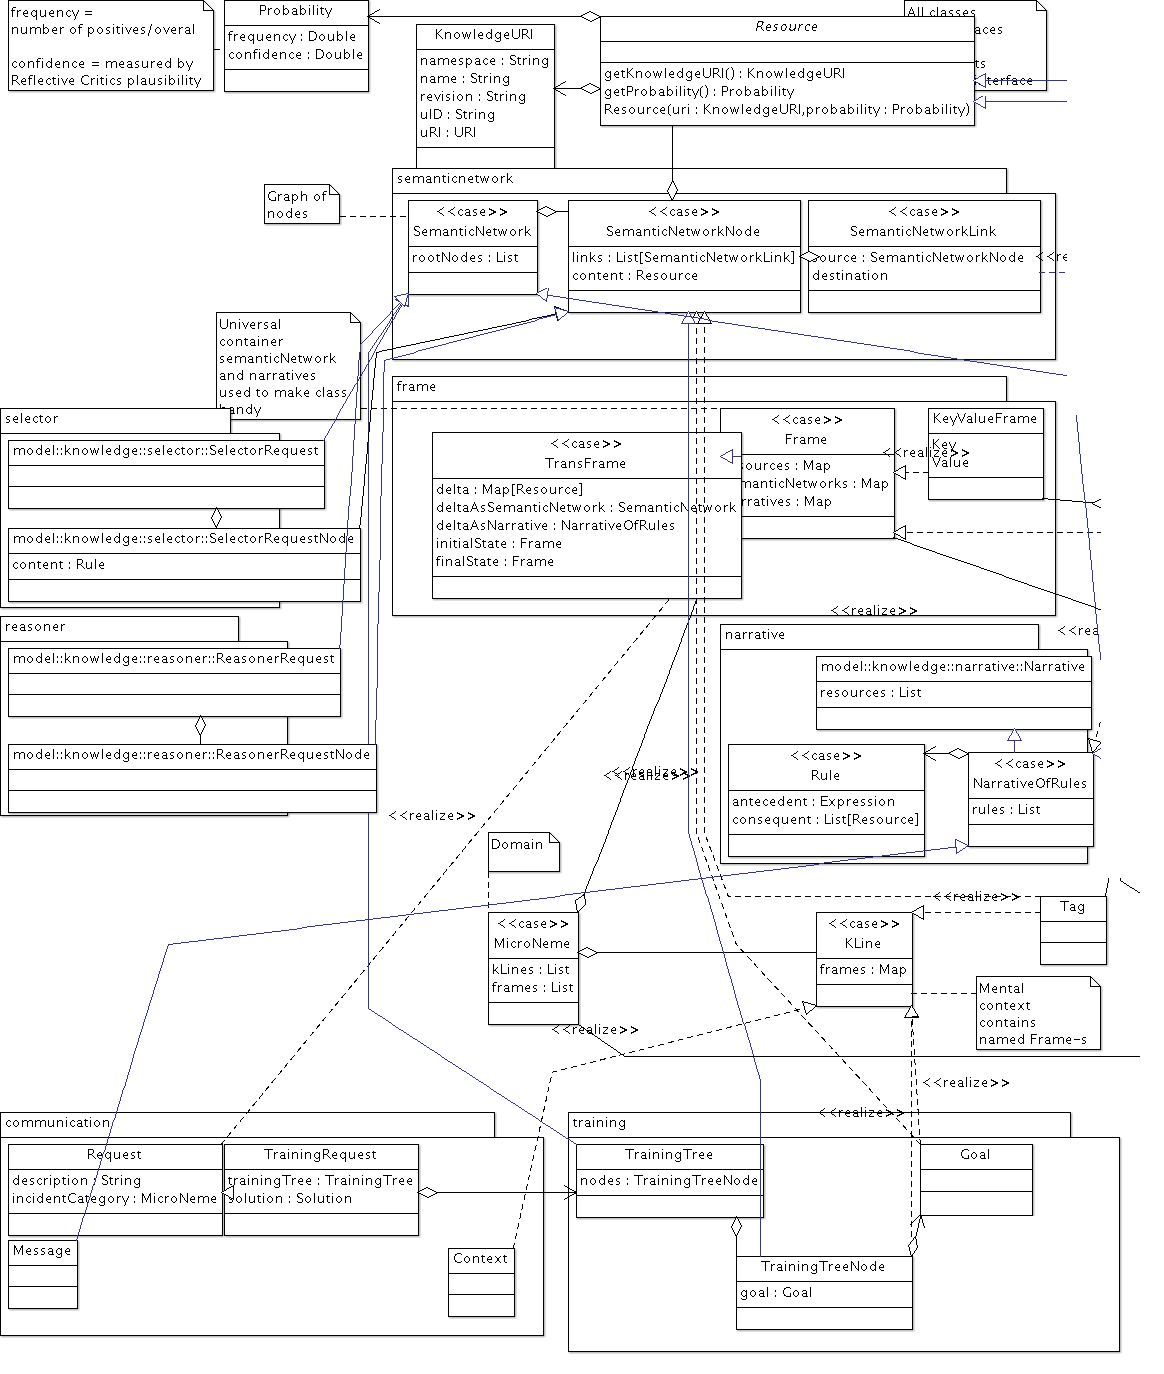
\includegraphics [scale=0.6] {KnowledgeClass}
  \caption{Схема данных TU Knowledge в формате UML} 
  \label{img:KnowledgeClass}  
\end{figure}
%\end{landscape}

\begin{longtable}{|p{5cm}|p{12cm}|}
 \caption[Описание классов TUKnowledge]{Описание классов TUKnowledge}\label{TUKnowledge} \\ 
 \hline
 
 \multicolumn{1}{|c|}{\textbf{Класс}} & \multicolumn{1}{c|}{\textbf{Описание}}  \\ \hline 
\endfirsthead
\multicolumn{2}{c}%
{{\bfseries \tablename\ \thetable{} -- продолжение}} \\
\hline \multicolumn{1}{|c|}{\textbf{Класс}} &
\multicolumn{1}{c|}{\textbf{Описание}}  \\ \hline 
\endhead

\endfoot

\hline \hline
\endlastfoot
\hline
   Knowledge  & Базовый класс всех объектов модели. Содержит в себе URI, по которому уникально идентифицируется. Поддерживает версионность. Свойствами данного объекта обладают все объекты системы. Также содержит Probability (Вероятность) и Confidence (Уверенность) поля. Например, когда в результате работу WayToThink получается Knowledge он имеет Confidence 0, так как он только что был сгенерирован, когда его проверит Critic на его состоятельность при помощи определенных в Critic правил, то он поставит ему не 0 Confidence \\
   \hline
   Narrative  & Список слов исходного запроса \\
   \hline
   Rule  & Правило. Класс описывающий правила в системы. Например, правило по которому сработает Critic \ref{Critic}  \\
   \hline
   AnnotatedNarrative  & Слова исходного запроса и их сопоставление на концепции в Базе Знаний \\
   \hline
   SemanticNetwork  & Граф из SemanticNetworkNode и SemanticNetworkLink \\
   \hline
   SemanticNetworkNode  & Узел графа SemanticNetwork, содержит в себе ссылки на другие узлы, а также ссылку на Knowledge \\
   \hline
   SemanticNetworkLink  & Ссылка в графе SemanticNetworkLink \\
   \hline
   Frame  & Коллекция объектов Knowledge, с возможностью назначения специального атрибута (тега) для семантической группировки \\
   \hline
   TransFrame  & Коллекция Frame, содержащая два состояния одного фрейма: до и после \\
   \hline
   Goal  & Цель. Приложение \ref{AppendixB} \\
   \hline
   Tag & То же, что и цель, но используется для меток \\
   \hline
   Preliminary annotation  & SemanticNetwork входного запроса \\
   \hline
   KnowledgeBase annotation  & SemanticNetwork с сопоставлением концепциям Базы Знаний \\
   \hline
   Domain model  & SemanticNetwork доменной модели \\
   \hline
   Situation model  & SemanticNetwork, часть DomainModel, созданной для обработки текущего запроса. Приложение \ref{AppendixB} \\
   \hline
   Incident  & SemanticNetwork входного запроса к систему \\
   \hline
   K-Line  & Связь между объектами. Например, когда в систему поступает запрос она создает K-Line между Conversation, Narrative \\
   \hline
   Conversation  & SemanticNetwork, контекст инцидента \\
   \hline
   InboundRequest  & SemanticNetwork входного запроса \\
   \hline
   Training Request  & SemanticNetwork входного запроса для обучений \\
   \hline
   
  \end{longtable}

\textbf{Описание запросов в рамках TU Knowledge} \par
В рамках модели данных TU Knowledge проблема имеет следующее описание:
\begin{itemize}
	\item Область (Микронема);
	\item Дата обращения;
	\item Автор;
	\item Приоритет;
	\item Категория;
	\item Теги;
	\item Описание.
\end{itemize}
Запрос на обучение включает следующие части:
\begin{itemize}
	\item Область (Микронема);
	\item Дерево обучения;
	\item Ограничения (например, время на решение).
\end{itemize} \par
 \textbf{Микронема} описывает контекст работы системы. В разрезе человеческого мышления это область работы мозга с нейронами и связями. Сочетание разных микронем может привести к изменению взглядов человека, характера, например, когда кто-то узнает новую идею и это заменяет его предыдущие представления о том или ином явлении. \par 

\textbf{Дерево обучения} базируется на структуре цель--подцель (см. приложение \ref{AppendixB}). Получение системой целей происходит из подцелей или при получении запроса пользователя. Например, при запросе пользователя устанавливается цель "Help User (Помочь пользователю)".\par

Во время процедуры обучения возможно, что на одном уровне окажется несколько целей, тогда необходимо провести дополнительное уточнение, если такое невозможно, то будет выбрана первая цель.


Во время работы MostProbableWay2Think может использовать несколько WayToThink, в таком случае он возьмет первый (наиболее вероятный путь). Если в результате его использования цель достигнута не будет, то будет выбран менее вероятный.

Пример
\begin{lstlisting}
 1. SubGoal = Resolve incident
   2. SubGoal = ParseIncidentDescription, Way2Think = ProcessText: KnowingHow, SemanticNetWorkWithKLines =
{
nsubj(received-3, User-1)
aux(received-3, had-2)
root(ROOT-0, received-3)
amod(application-5, wrong-4)
dobj(received-3, application-5)

advmod(received-3, However-1)
nsubj(received-3, user-2)
ccomp(received-8, received-3)
amod(version-5, wrong-4)
dobj(received-3, version-5)
nsubj(received-8, user-7)
root(ROOT-0, received-8)
nn(Tehcnical-10, Wordfinder-9)
dobj(received-8, Tehcnical-10)
advmod(of-12, instead-11)
prep(Tehcnical-10, of-12)
nn(Economical-14, Business-13)
pobj(of-12, Economical-14)
}
   2. SubGoal = UnderstandIncidentType, Critics = Deliberative, Type = ProblemDescription with DesiredState
     3. SubGoal = ModelCurrentSituation using ProjectDomain Model, Way2Think = Simulate, Model =
{
User Desired(ordered) Soft(Wordfinder Business Economical)
Operator Installed Soft(Wordfinder Tehcnical) - wrongly
}
     3. SubGoal = FormalizeProblemDescription using ProblemModel(Wrong state, Desired state), Way2Think = Reformulate, Model=
{
WrongState = Soft.installed(Wordfinder Tehcnical), Soft.notInstalled(Wordfinder Business Economical)
DesiredState = Soft.installed(Wordfinder Business Economical), Soft.unInstalled(Wordfinder Tehcnical)
}
     3. SubGoal = Find solution, Way2Think = ExtendedSearch, Solution =
     { Install(Wordfinder Business Economical), UnInstall(Wordfinder Tehcnical)}
     
\end{lstlisting}
\clearpage

\section{Прототип системы}
В прототипе были реализованы 4 уровня мышления. Ниже описан стандартный поток системы, который дает возможность понять основной принцип работы.
\begin{enumerate}
	\item Поступает запрос пользователя: 
	"User had received wrong application. User has ordered Wordfinder Business Economical. However she received wrong version, she received Wordfinder Tehcnical instead of Business Economical. Please assist."\ («Пользователь получил неверное приложение. Пользователь заказал приложение "Wordfinder. Бизнес версия"\,, но получил неверную версию,~--- "Wordfinder. Техническая версия". Пожалуйста, помогите»);
	\item Компонент GoalManger (Менеджер целей) устанавливает цель системы HelpUser (Помочь пользователю);
	\item Главный компонент Thinking Life Cycle (далее TLC) активирует набор компонетов Critic (Критик), привязанный к данной цели (HelpUser); 
	\item Активируется компонент PreliminaryAnnorator (Предварительный обработчик), который разбирает запрос, проводя орфографическую коррекцию и предварительный разбор;
	\item Компонент KnowledgeBaseAnnotator (разбор при помощи накопленных знаний) создает семантическую сеть и ссылки на нее;
	\item Компонент Critic (Критик), привязанный к цели HelpUser на Рефлексивном уровне, запускает WayToThink (Образ мышления) ProblemSolving (Разрешить проблемную ситуацию) с целью: ResolveIncident;
	\item Компонент Critic на Рефликсивном уровне выбирает WayToThink KnowingHow (Поиск рецепта решения);
	\begin{enumerate}
	\item Запускаются параллельно все компоненты класса Critic, которые привязаны к цели ResolveIncident (Решить проблему), в данном случае это DirectInstruction (прямые инструкции), ProblemWithDesiredState (проблемы с желаемым состоянием), ProblemWithoutDesiredState (проблема без желаемого состояния);
	\item Компонент Selector (Селектор) выбирает среди всех результатов наиболее вероятный результат работы. В данном случае им будет Problem Description with desired state (Проблема с желаемым состоянием);
	\item Компонент KnowingHow сохраняет варианты выбора Selector;
	\item Компонент Simulation (Моделирование) WayToThink с параметрами «создать модель текущий ситуации» создает: концепцию существующей ситуации (CurrentState), концепцию пользователя, концепцию программного обеспечения;
	\item Компонент Reformulation WayToThink (Компонент дополнения), используя результаты предыдущего шага, синтезирует артефакты, которых не хватает, чтобы получить из CurrentState DesiredState (Желаемое состояние), так как он не указан явно. WayToThink запускает Critic размышления, чтобы найти корень проблемы. Он находит CurrentState (настоящее состояние)~--- Wordfinder Tehcnical и DesiredState (состояние, которое нужно пользователю)~--- Wordfinder Business Economical;
	\item Рефлексивные Critic оценивают состояние системы~--- на каком шаге она находится, и если цель не достигнута, то запускают другой WayToThink, например, DirectInstruction;
	\item Компонент Critic Solution Generator (Компонент генерации решения) запускает KnowingHow WayToThink, ExtensiveSearch (Поиск решения);
	\item Компонент Selector выбирает наиболее вероятный образ мышления. В данном случае это будет ExtensiveSearch, который будет находить решения, позволяющие привести систему в необходимое пользователю состояние (DesiredState), если сделать это невозможно, то система инициирует коммуникацию с пользователем. 
 \end{enumerate}
	 \item Рефлексивный Critic проверяет состояние системы. Если Цель достигнута, то пользователю посылается ответ.
	 \item На данном шаге активируются компоненты класса Critic на cамосознательном уровне, которые сохраняют информацию о затратах на решение.
  \end{enumerate}\par

На рисунке \ref{img:LifecycleActivity} представлена UML-диаграмма действий системы согласно алгоритму, описанному выше и с привязкой к уровням мышления.
\begin{figure} [h] 
  \center
  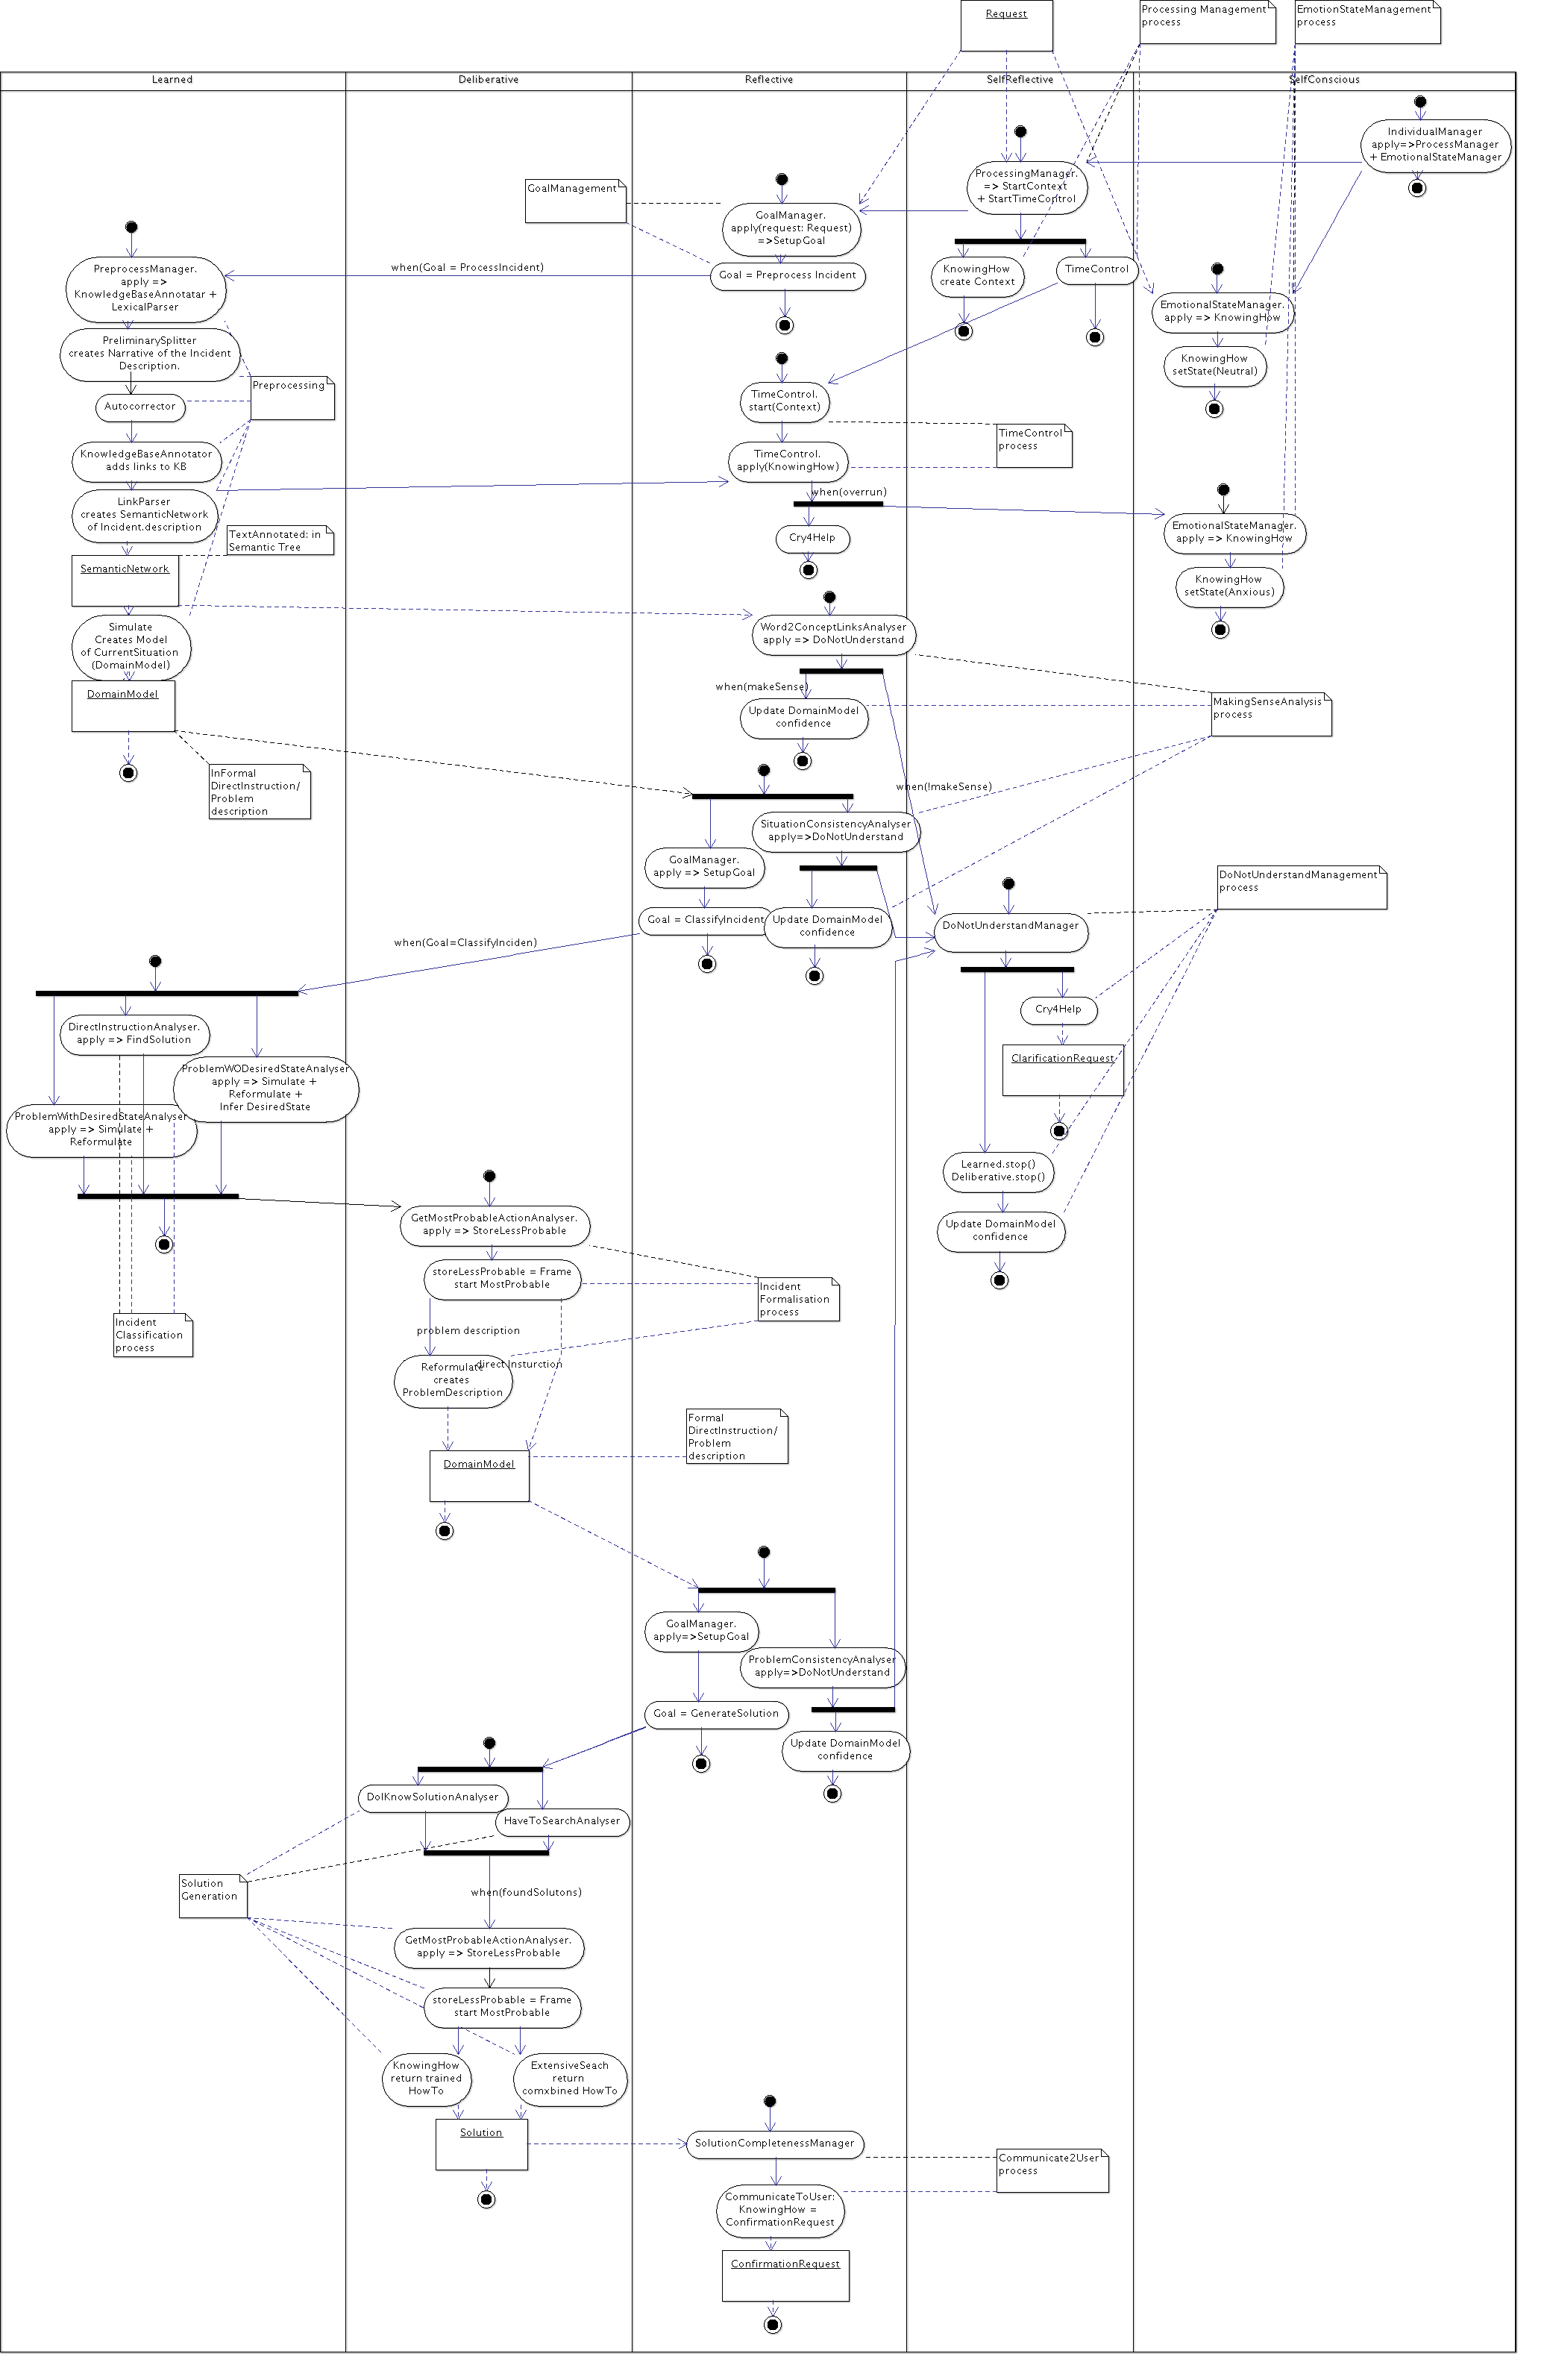
\includegraphics [scale=0.2] {LifecycleActivity}
  \caption{Диаграмма действий LifecycleActivity} 
  \label{img:LifecycleActivity}  
\end{figure}
\clearpage

\section{Выводы по главе 3}
В данной главе рассмотрены:
\begin{itemize}
	\item архитектура системы по модели TU;
	\item модель данных TU Knowledge;
	\item реализация системы;
	\item состав прототипа;
	\item основной поток действий системы.
\end{itemize} \par
Кроме того, приведены алгоритмы и методы, использованные при создании системы; рассмотрены технологии, использованные при создании прототипа. Для удобства основные диаграммы выполнены с использованием универсального формата UML 2.0. Продемонстрированы основные потоки работы как для каждого компонента, так и для всех компонентов в целом. \par
По данной архитектуре была выполнена программная реализация с использованием функционального языка Scala. Основной платформой для эксплуатации системы был выбран Debian дистрибутив системы Linux, точнее, Ubuntu 12 (и выше). Связано это, прежде всего, с тем, что ряд компонентов был написан на С++ и использует библиотеки, доступные только на Linux.  \par
Система была протестирована на экспериментальных данных, которые представлены в Приложении \ref{AppendixE} и предоставлены \icl, о чем свидетельствует акт о внедрении (см. Приложение \ref{AppendixG}).


\clearpage           % Глава 3
\chapter{Экспериментальные исследования эффективности работы модели TU}


%================================
%================================
%================================
\section{Экспериментальные данные}
В качестве экспериментальных данных были взяты выгрузки проблем из информационных систем \icl. 
Для начального обучения в систему заложено две базовые концепции: Object~--- объект, который является базовой концепцией для всех объектов, и Action~--- действие, которое является базовой концепцией для всех действий. 
В таблице \ref{Test data description} представлен список основных тренировочных данных.

\begin{longtable}{|p{12cm}|p{5cm}|}
 \caption[Описание экспериментальных данных]{Описание экспериментальных данных}\label{Test data description} \\ 
 \hline
 
 \multicolumn{1}{|c|}{\textbf{Входное предложение}} & \multicolumn{1}{c|}{\textbf{Описание}}  \\ \hline 
\endfirsthead
\multicolumn{2}{c}%
{{\bfseries \tablename\ \thetable{} -- продолжение}} \\
\hline \multicolumn{1}{|c|}{\textbf{Входное предложение}} &
\multicolumn{1}{c|}{\textbf{Описание}}  \\ \hline 
\endhead

\endfoot

\hline \hline
\endlastfoot
\hline
  Tense is kind of concept~(Время~--- это концепция).  & Обучающий запрос. Создает связь между концепцией Tense и Concept \\
  
  \hline
   Please install Firefox~(Установите Firefox).  & Запрос. Пользователь просит установить Firefox. Результатом должен быть найдено решение по установки Firefox \\
  \hline
  Browser is an object~(Браузер~--- это объект).   & Обучающий запрос. Создает связь между концепцией Browser и object \\
  \hline
  Firefox is a browser~(Firefox~--- это браузер).   & Обучающий запрос. Создает связь между концепцией Firefox и browser  \\
  \hline
  Install is an action~(Установить~--- это действие).    & Обучающий запрос. Создает связь между концепцией Install и action \\
  \hline
  User miss Internet Explorer 8~(У пользователя нет Internet Explorer 8).      & Запрос. Проблема с желаемым состоянием (DesiredState) \\
  \hline
  User needs document portal update~(Пользователю требуется обновление документов).    & Запрос. Проблема с желаемым состоянием \\
  \hline
 Add new alias Host name on host that alias is wanted to: hrportal.lalala.biz IP address on host that alias is wanted to: 322.223.333.22 Wanted Alias:    webadviser.lalala.net~(Добавьте, пожалуйста, новую ссылку на hrportal.lalala.biz через 322.223.333.22).    & Запрос. Сложная проблема  \\ 
  \hline
   Outlook Web Access (CCC)~--- 403~--- Forbidden: Access is denied~(Нет доступа к Outlook Web Access (CCC)). & Сложная проблема \\ 
  \hline
  PP2C~--- Cisco IP communicator. Please see if you can fix the problem with the ip phone, it's stuck on configuring ip + sometimes Server error rejected: Security etc~(PP2C~--- коммуникатор Cisco IP. Пожалуйста, помогите исправить проблему с ИП-телефоном, он застревает во время конфигурирования и иногда показывает ошибку «Безопасность»).     & Запрос. Сложная проблема \\ 
   \hline
  \end{longtable}

Полный список информации об экспериментальных данных представлен в приложении \ref{AppendixE}.




%================================
%================================
%================================
\section{Оценка эффективности}
Для верификации экспертной системы поддержки принятия решений TU была выбрана область поддержки информационной инфраструктуры предприятия, которая в рамках работы исследована и смоделирована в Главе \ref{chapt1}. 
Для доказательства жизнеспособности решения производилась верификация в 2 этапа:
\begin{itemize}
	\item Этап 1. Разбор входящего запроса на естественном языке и вычленение концепции;
	\item Этап 2. Обработка по разработанной архитектуре и реализации модели мышления.  
\end{itemize} \par
Для Этапа 1 использовалась отфильтрованная выгрузка инцидентов. Были выявлены уникальные инциденты~--- 1000. На данном этапе удалось добиться качества разбора на уровне 67\%. Успешным считался разбор, когда правильно были определены концепции, например, существительное определялось как существительное, глагол как глагол. \par
Для Этапа 2 использовалась часть инцидентов, которая представлена в предыдущий главе. На них запускался программный комплекс и анализировались результаты. Удалось добиться 95\% успешных инцидентов. Успешным считался инцидент, который был успешно сопоставлен концепциям в базе знаний. \par
Результатом успешной обработки инцидента считалось найденное решение, если же решения не было, то проверялось правильное понимание системой всех концепций, так как решения не было в базе знаний. Запуск работы системы производился при помощи автоматизированных тестов. Проверка данных также осуществлялась при помощи этой технологии. Система также может функционировать в режиме диалога и в консольном варианте, в этом режиме видно взаимодействие с пользователем. 



%================================
%================================
%================================
\section{Результаты экспериментов}

Система показала свою жизнеспособность на модельных данных. Были проведены тесты в сравнении с работой человеческого специалиста. Был выбран контрольный список инцидентов. Сравнивался поиск решения для инцидентов. Основное время при опросе специалиста тратилось на коммуникацию. В Таблице \ref{HumanComparison} приведены результаты сравнения. Тесты были выполнены на компьютере Intel Core i7 1700 MHz, 8GB RAM, 256 GB SSD, FreeBSD. 
\begin{longtable}{|p{12cm}|p{2cm}|p{2cm}|}
 \caption[Результаты сравнения с работой специалиста]{Результаты сравнения с работой специалиста}\label{HumanComparison} \\ 
 \hline
 
 \multicolumn{1}{|c|}{\textbf{Инцидент}} & \multicolumn{1}{c|}{\textbf{TSS1 (.мс)}} & \multicolumn{1}{c|}{\textbf{TU (.мс)}}  \\ \hline 
\endfirsthead
\multicolumn{2}{c}%
{{\bfseries \tablename\ \thetable{} -- продолжение}} \\
\hline \multicolumn{1}{|c|}{\textbf{Инцидент}} & \multicolumn{1}{c|}{\textbf{TSS1 (.мс)}} & \multicolumn{1}{c|}{\textbf{TU (.мс)}}  \\ \hline 
\endhead

\endfoot

\hline \hline
\endlastfoot
\hline
  Tense is kind of concept~(Время~--- это концепция) & 15000 & 385 \\
  
  \hline
  Please install Firefox~(Установите Firefox)   & 9000 & 859 \\
  \hline
  Browser is an object~(Браузер~--- это объект)   & 20000 & 400 \\
  \hline
  Firefox is a browser~(Firefox~--- это браузер)   & 5000 & 659  \\
  \hline
  Install is an action~(Установить~--- это действие)   & 8000 & 486 \\
  \hline
  User miss Internet Explorer 8~(У пользователя нет Internet Explorer 8)     & 10000 & 10589 \\
  \hline
  User needs document portal update~(Пользователю требуется обновление документов)    & 15000 & 16543 \\
  \hline
  Add new alias Host name on host that alias is wanted to: hrportal.lalala.biz IP address on host that alias is wanted to: 322.223.333.22 Wanted Alias:    webadviser.lalala.net~(Добавьте, пожалуйста, новую ссылку на hrportal.lalala.biz через 322.223.333.22)    & 10000 & 18432  \\ 
  \hline
  Outlook Web Access (CCC)~--- 403~--- Forbidden: Access is denied~(Нет доступа к Outlook Web Access (CCC)) & 15000 & 10342\\ 
  \hline
  PP2C~--- Cisco IP communicator. Please see if you can fix the problem with the ip phone, it's stuck on configuring ip + sometimes Server error rejected: Security etc~(PP2C~--- коммуникатор Cisco IP. Пожалуйста, помогите исправить проблему с ИП-телефоном, он застревает во время конфигурирования и иногда показывает ошибку «Безопасность»)  & 13000 & 12343 \\ 
   
  \end{longtable}


Основной проблемой для системы составляют инциденты с большой неоднозначностью, например, "I should have Internet Explorer, but Firefox was installed". Здесь непонятно, нужен ли пользователю браузер Firefox или нет. В этом случае система должна выявить проблему о необходимости пользователю Internet Explorer. \par 
Другой пример, который трудно однозначно решить, используя классические подходы: I install Internet Explorer previously, but i need Chrome. Здесь есть следующие наборы концепций: i, install, Internet Explorer; i, need, Chrome. Используя регулярные выражения, однозначно решить не удастся, но, используя интеллектуальное решение, эту проблему решить можно. В рамках TU сработает более вероятный Critic, который определит проблему "need Chrome"\,, базируясь на наличии концепции "previously". 
В таблице  \ref{ProblemClassComparison} приведены результаты работы системы в разрезе категорий инцидентов. \\

\begin{longtable}{|p{12cm}|p{5cm}|}
 \caption[Описание экспериментальных данных]{Описание экспериментальных данных}\label{ProblemClassComparison} \\ 
 \hline
 
 \multicolumn{1}{|c|}{\textbf{Класс проблемы}} & \multicolumn{1}{c|}{\textbf{
 \% успешных}}  \\ \hline 
\endfirsthead
\multicolumn{2}{c}%
{{\bfseries \tablename\ \thetable{} -- продолжение}} \\
\hline \multicolumn{1}{|c|}{\textbf{Входное предложение}} &
\multicolumn{1}{c|}{\textbf{Описание}}  \\ \hline 
\endhead

\endfoot

\hline \hline
\endlastfoot
\hline

Проблема с ПО    & 64\% \\
 \hline Проблемы во время работы  &  10\% \\
  \hline Как сделать & 10\% \\
   \hline
Проблема с оборудованием  & 0\% \\
 \hline
Установить новое ПО       & 100\% \\
 \hline Проблема с печатью        & 80\% \\
  \hline Нет доступа               & 100\% \\
  \hline
  \end{longtable}
  


  
Показатели, приведенные в главе 1, $\alpha$ --- доля заявок, для которых время в очереди превышает $max(T_q)$;       
$\mu$ --- величина, обратная среднему времени нахождения заявки у агента;
$n$ --- число агентов;
$T_q$ --- время нахождение заявки в очереди в часах;
$SLA$ --- уровень обслуживания (1-$\alpha$), доля заявок, для которых время в очереди не превышает $max(T_q)$. $T_p$ --- время удовлетворения заявки;
 $\alpha_n$ --- количество заявок;
 $T_{qp}=T_q+T_p$ --- время прохождения заявки через систему,
 приобрели следующие значения $T_qp=32,9$ при $n=8$; $SLA=0,96$; $\alpha=0,04$;  $\alpha_n=2920$.  Предыдущие значение было $T_{qp}=47,9$ при $n=6$; $SLA=0,82$; $\alpha=0,18$;  $\alpha_n=2920$, но увеличение $n$ не привело к увеличению задействованных в работе специалистов. Согласно таблице \ref{ProblemClassComparison} средний процент обработанных заявок составил 52\%, что составляет более половины всех заявок и требуемых 30\% (см. Главу 1).

  
\section{Выводы по главе 4}
В главе рассмотрены экспериментальные данные, которые были использованы для верификации системы, также дается обоснование, почему были выбраны именно эти данные. На основе экспериментов была посчитана скорость работы системы в сравнении со специалистом технической поддержки. Были приведены сложные для решения примеры входных запросов пользователя и дан их разбор. 


\clearpage           % Глава 4
\chapter*{Заключение}						% Заголовок
\addcontentsline{toc}{chapter}{Заключение}	% Добавляем его в оглавление

%% Согласно ГОСТ Р 7.0.11-2011:
%% 5.3.3 В заключении диссертации излагают итоги выполненного исследования, рекомендации, перспективы дальнейшей разработки темы.
%% 9.2.3 В заключении автореферата диссертации излагают итоги данного исследования, рекомендации и перспективы дальнейшей разработки темы.
%% Поэтому имеет смысл сделать эту часть общей и загрузить из одного файла в автореферат и в диссертацию:

%% Согласно ГОСТ Р 7.0.11-2011:
%% 5.3.3 В заключении диссертации излагают итоги выполненного исследования, рекомендации, перспективы дальнейшей разработки темы.
%% 9.2.3 В заключении автореферата диссертации излагают итоги данного исследования, рекомендации и перспективы дальнейшей разработки темы.

Решены следующие задачи и достигнуты следующие результаты.
\begin{enumerate}
  \item Создана модель проблемно-ориентированной системы управления знаниями в области обслуживания информационной инфраструктуры предприятия на основе обобщения модели мышления;
  \item Представлены новая модель данных для модели мышления и оригинальный способ их хранения, более эффективный по сравнению с классическими базами данных, использующими реляционный подход;
  \item Выполнено оригинальное исследование моделей мышления в области обслуживания информационной инфраструктуры предприятия;
  \item На основе модели, разработанной в диссертации, созданы архитектура системы и ее прототип; 
  \item Система, разработанная в рамках данной работы, включает в себя инновационные методы и алгоритмы поддержки принятия решений, использует обобщенную модель мышления Мински;
  \item Представлена визуализация структуры области удаленной поддержки инфраструктуры.
\end{enumerate}

Представленные в диссертации модель мышления, ее архитектура и реализация являются уникальными~--- на данный момент времени это единственная реализация модели мышления Мински. \par
Система, разработанная в диссертации, не является узкоспециализированной и подходит для других областей, где требуется организация базы знаний, например, при постановке медицинского диагноза, чтобы отбросить ложные диагнозы. \par
В области диагностики проблем можно обучить систему сведениям об узлах автомобиля и проблемах, с ними связанных, признаках этих проблем и способах их устранения. \par
Работа выполнена  частично за счет средств субсидии, выделенной Казанскому федеральному университету для выполнения государственного задания в сфере научной деятельности, проекты 1.2368.2017, «Бюджет 17-97».






Работа велась с использованием открытых технологий, без использования проприетарного программного обеспечения.  
Работа выполнялась при помощи компании \icl, в рамках работы использовались и обрабатывались данные, собранные во время работы команд \icl\  над поддержкой информационной структуры предприятий-заказчиков.      % Заключение
\chapter*{Список сокращений и условных обозначений} \label{acronyms}             % Заголовок
\addcontentsline{toc}{chapter}{Список сокращений и условных обозначений}  % Добавляем его в оглавление

\textbf{selectLinkedObject(obj:Resource, linkName:String): Link<Resource>}~--- Описание метода. selectLinkedObject~--- название метода. (obj:Resource, linkName:String)~--- параметры метода. linkName~--- имя параметра. String тип данных. Link<Resource>~--- тип возвращаемых данных. Если метод данных не возвращает, то ничего не указывается.\par
\textbf{DomainModel:SemanticNetwork}~--- Описание класса, где DomainModel~--- сам класс, а SemanticNetwork~--- класс-родитель.\par
\textbf{TU}~--- Сокращение от ThinkingUnderstanding.\par
\textbf{TLC}~--- Thinking Life Cycle.\par
\textbf{НДФЛ}~--- Налог на доходы физически лиц.\par
\textbf{ПО}~--- Программное обеспечение.\par
\textbf{ФБ}~--- Федеральный бюджет.\par
\textbf{ПФР}~--- Пенсионный фонд России.\par
\textbf{ТФОМС}~--- Территориальный фонд обязательного медицинского страхования.\par
\textbf{ФФОМС}~--- Федеральный фонд обязательного медицинского страхования.\par
\textbf{ФСС}~--- Фонд социального страхования.\par
\textbf{БД}~--- База данных.\par
\textbf{мс.}~--- Миллисекунды.\par


\clearpage
      % Список сокращений и условных обозначений
\chapter*{Словарь терминов} \label{Glossary}            % Заголовок
\addcontentsline{toc}{chapter}{Словарь терминов}  % Добавляем его в оглавление

\textbf{База Знаний}~--- База данных приложения, представленная в виде онтологии знаний. \par
\textbf{WayToThink}~--- Путь мышления. Основан на определении Марвина Мински \cite{EmotionMachine}. Класс объектов, которые модифицируют данные. \par
\textbf{Critic}~--- Основан на определении Марвина Мински \cite{EmotionMachine}. Класс объектов, которые выступают триггерами при наступление определенного события. \par
\textbf{ThinkingLifeCycle}~--- Основан на определении Марвина Мински \cite{EmotionMachine}. Класс объектов, которые выступают основными объектами для запуска в приложении~--- рабочими процессами. \par
\textbf{Selector}~--- Компонент, отвечающий за выборку данных из Базы Знаний. \par
\textbf{Instinctive}~--- Инстинктивный уровень. \par
\textbf{Learned}~--- Уровень обученных реакций. \par
\textbf{Deliberative}~--- Уровень рассуждений. \par
\textbf{Reflective}~--- Рефлексивный уровень. \par
\textbf{Self-Reflective Thinking	}~--- Саморефлексивный уровень. \par
\textbf{Self-Conscious Reflection}~--- Самосознательный уровень. \par
\textbf{ThinkingUnderstanding}~--- Система, созданная в рамках работы. Дословный перевод «Мышление-Понимание».\par  
\textbf{Вариант использования}~--- Термин из стандарта UML, который описывает возможные способы функционирования системы.\par  
\textbf{Диаграмма действий}~--- Термин из стандарта UML, который описывает последовательность действий пользователя.\par  
 
\clearpage    % Словарь терминов
\clearpage
\phantomsection
\addcontentsline{toc}{chapter}{\bibname}	% Добавляем список литературы в оглавление
\insertbiblioall{}					% Подключаем BibTeX-базы      % Список литературы
\clearpage
\phantomsection
\addcontentsline{toc}{chapter}{\listfigurename}
\listoffigures									% Список изображений
\newpage

%%% Список таблиц %%%
% (ГОСТ Р 7.0.11-2011, 5.3.10)
\clearpage
\phantomsection
\addcontentsline{toc}{chapter}{\listtablename}
\listoftables									% Список таблиц
\newpage           % Списки таблиц и изображений (иллюстративный материал)
\appendix
%% Правка оформления ссылок на приложения:
%http://tex.stackexchange.com/questions/56839/chaptername-is-used-even-for-appendix-chapters-in-toc
%http://tex.stackexchange.com/questions/59349/table-of-contents-with-chapter-and-appendix
%% требует двойной компиляции
\addtocontents{toc}{\def\protect\cftchappresnum{\appendixname{} }%
\setlength{\cftchapnumwidth}{\widthof{\cftchapfont\appendixname~Ш\cftchapaftersnum}}%
}
%% Оформление заголовков приложений ближе к ГОСТ:
\sectionformat{\chapter}[display]{% Параметры заголовков разделов в тексте
    label=\chaptertitlename\ \thechapter,% (ГОСТ Р 2.105, 4.3.6)
    labelsep=20pt,
}
\renewcommand\thechapter{\Asbuk{chapter}} % Чтобы приложения русскими буквами нумеровались

%=======================
%======APPENDIX A=======
%=======================
\chapter{Интерфейсная модель} \label{AppendixA}

Интерфейсная модель содержит классы и интерфейсы для взаимодействия с пользователем. На рисунке \ref{img:interface-model} представлена диаграмма классов модели данных. В ее основе лежит базовый объект RefObject, который объединяет в себе свойства, присущие всем объектам системы:
\begin{itemize}
	\item ObjectID~--- уникальный идентификатор объектах в пределах класса объекта;
	\item Reference~--- уникальный идентификатор объектах в пределах всей Базы Знаний;
	\item Name~--- имя объекта.
\end{itemize}

\begin{figure} [h] 
  \center
  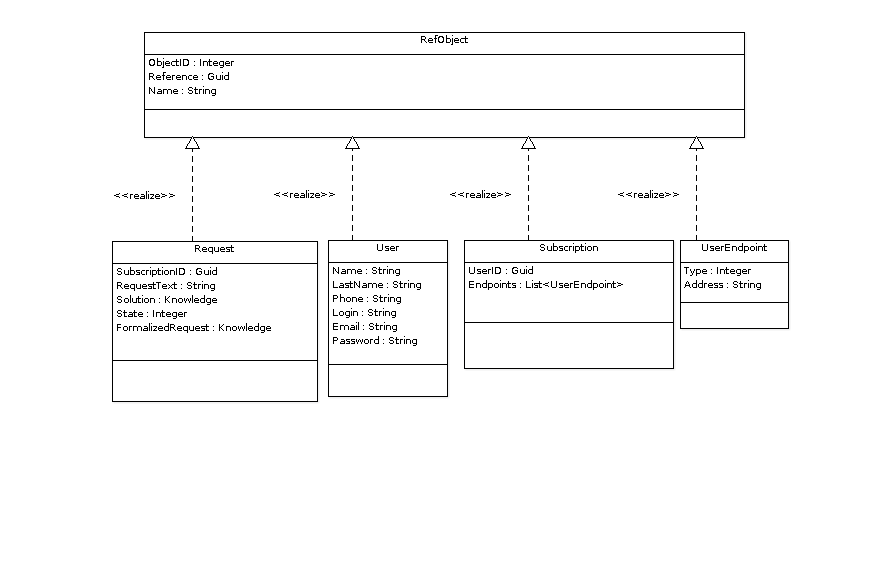
\includegraphics [scale=0.8,angle=90, origin=c] {interface-model}
  \caption{Диаграмма классов интерфейсной модели} 
  \label{img:interface-model}  
\end{figure}

Рассмотрим несколько объектов, например, Request (Запрос). Он предназначен для хранения запроса пользователя:
\begin{itemize}
	\item SubscriptionID~--- идентификатор подписки, ссылка на сущность Subscription (подписка);
	\item RequestText~--- запрос пользователя в виде текста;
	\item Solution~--- описание решения запроса пользователя;
	\item State~--- статус запроса (например, «поиск решения»);
	\item FormalizedRequest~--- ссылка на формализованный запрос.
\end{itemize} \par
Subscription (подписка) содержит информацию о подписке пользователя на информирование о событиях. Список точек оповещения (Endpoints), благодаря которым система будет предоставлять информацию пользователю о состоянии его запроса. Точка оповещения описывается набором параметров из Type (тип)~--- тип точки связи с пользователем (например, веб-сервис) и Address (адрес)~--- адрес точки связи с пользователем.

%=======================
%======APPENDIX B=======
%=======================
\chapter{Описание модуля Goal (Цель) и Action (Действия)} \label{AppendixB}
Action (Действие) является базовым классом для WayToThink или Critic. Он описывает общие методы этих классов: start (запуск); stop (остановка) и apply (применение)~--- метод, который производит работу над контекстом и изменяет данные. На рисунку \ref{img:ActionClass} представлена диаграмма классов Action, где отображена связь с Critic и WayToThink.
\begin{figure} [h] 
  \center
  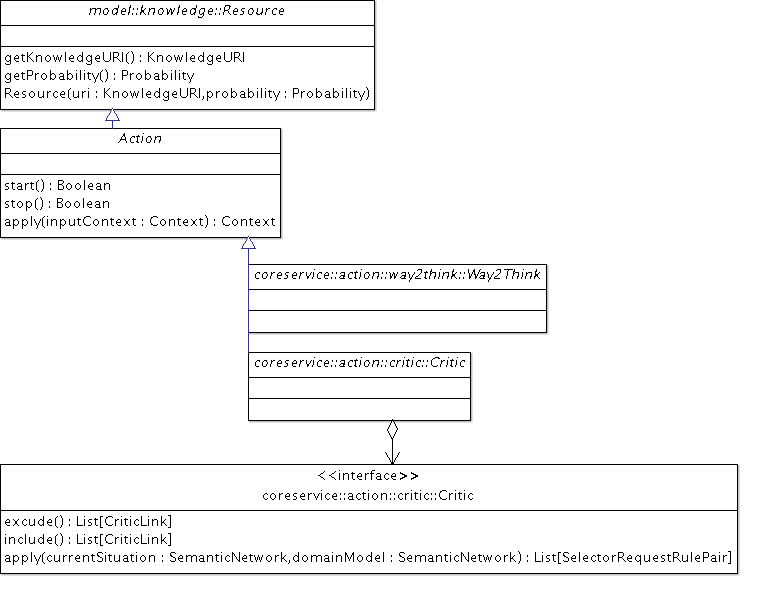
\includegraphics [scale=0.65] {ActionClass}
  \caption{Диаграмма классов Action} 
  \label{img:ActionClass}  
\end{figure}

Goal (Цель) является набором вероятностных предикатов и последовательностью How-To необходимых для того, чтобы достичь цель. Goal и How-To тесно связаны. На рисунке \ref{img:goal} показан состав Goal. Goal состоит из:
\begin{enumerate}
	\item Parameters~--- параметры, которые используются предикатами для выполнения;
	\item Precondition~--- условия, которые должны быть выполнены до начала основной проверки (Exit criteria);
	\item Entry criteria~--- входной критерий, предикат, который определяет, что цель активировалась;
	\item Exit criteria~--- условия, когда цель считается выполненной;
	\item PostCondition~--- дополнительные условия для выхода;
	\item HowTo~--- набор решения. Список путей решения.
\end{enumerate}

\begin{figure} [h] 
  \center
  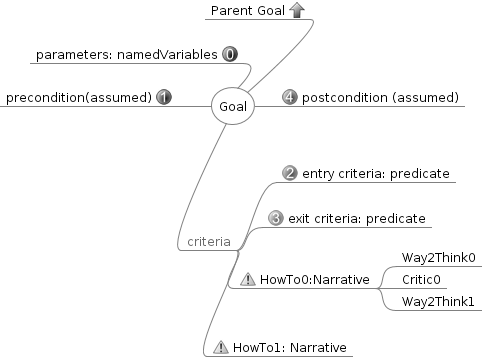
\includegraphics [scale=1.0, origin=c] {goal}
  \caption{Диаграмма классов Goal} 
  \label{img:goal}  
\end{figure} \par
\clearpage
\textbf{Типы предикатов}. В решении используется 3 типа логических предикатов: and (и), or (или), not (отрицание). Представление Goal в SemanticNetwork показано на диаграмме \ref{img:2_0_GoalHowToConcept}.

\begin{figure} [h] 
  \center
  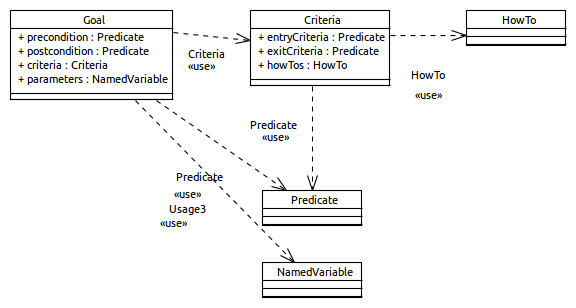
\includegraphics [scale=1.0, origin=c] {2_0_GoalHowToConcept}
  \caption{Диаграмма места Goal в SemanticNetwork (Семантической сети)} 
  \label{img:2_0_GoalHowToConcept}  
\end{figure}

Основная цель системы~--- помочь пользователю. Все остальные цели являются подцелями основной: разрешить инцидент, понять тип инцидента, найти решение инцидента \etc.

%=======================
%======APPENDIX D=======
%=======================
\chapter{Рецепты решений} \label{AppendixDHowTo}
Рецепты решений представляют собой последовательность действий выполняемых для разрешения проблемы, описанной в инциденте. 
Было разработано два типа HowTo (рецепт решения): ValueHowTo~--- содержит в себе простое значение; FunctionalHowTo~--- содержит в себе функцию. \par
FunctionalHowTo состоит из следующих частей:
\begin{enumerate}
	\item FunctionalBody~--- тело функции, описывающий содержание функции;
	\item InputParameters~--- входные параметры функции;
	\item OutputParameters~--- выходные параметры.
\end{enumerate} \par
Комбинация FunctionaHowTo и ValueHowTo является рецептом решения. Например, решение проблемы неработающего сегмента кластера в формате для специалиста технической поддержки.
\begin{itemize}
	\item Войти на сервер U1;
	\item Запустить утилиту 12 для Windows Servers;
	\item Открыть вкладку 1;
	\item Перейти на All Managed Server, найти нужный Server из правой панели, открыть свойства сервера;
	\item Нажать на Backup Exec Services;
	\item Выберите проблемный сегмент кластера;
	\item Нажмите Restart all Services;
	\item Подождите и проверьте статус.
\end{itemize} \par
Преобразованный в формат HowTo данный рецепт решения будет выглядеть как показано ниже.

\begin{lstlisting}
	login:howto{
  Parameters:[

    {Key:'ScriptName',
    Value:'LogonScript.bat'},
    {Key:'Description',
    Value:'Logon to server'}
  ]

  InputParameters:[
    {Key:'ServerName',
    Value:'U1'},
    {Key:'UserName',
    Value:'MyUser'}
  ]

  OutputParameters:[
    {Key:'SessionID',
    Value:'SSSE12'},

  ]
}

launch:howto{
  Parameters:[

    {Key:'ScriptName',
    Value:'LaunchScript.bat'},
    {Key:'Description',
    Value:'Launch the application'}
  ]

  InputParameters:[
    {Key:'ExecName',
    Value:'Utility12.exe'},
  ]

  OutputParameters:[
    {Key:'SessionID',
    Value:'SSSE12'},

  ]
}
\end{lstlisting}
%=======================
%======APPENDIX E=======
%=======================
\clearpage
\chapter{Экспериментальные данные}\label{AppendixE}
Здесь приведена лишь часть экспериментальных данных (Общая длина файла примерно 10000 инцидентов). 
\begin{longtable}{|p{5cm}|p{6cm}|p{5cm}|}
 \caption[Описание экспериментальных данных]{Описание экспериментальных данных}\label{ExpData} \\ 
 \hline
 
 \multicolumn{1}{|c|}{\textbf{Класс проблемы}}& \multicolumn{1}{c|}{\textbf{
 Описание проблемы}} & \multicolumn{1}{c|}{\textbf{
 \% успешных}}  \\ \hline 
\endfirsthead
\multicolumn{2}{c}%
{{\bfseries \tablename\ \thetable{} -- продолжение}} \\
\hline \multicolumn{1}{|c|}{\textbf{Входное предложение}} &
\multicolumn{1}{c|}{\textbf{Описание}}  \\ \hline 
\endhead

\endfoot

\hline \hline
\endlastfoot
\hline

Проблема с ПО   &  & 64\% \\
 \hline Проблемы во время работы &  &  10\% \\
  \hline Как сделать&  & 10\% \\
    \hline         &    Hi NAS Admin,Please connect following groups to the shared disk listed below and configure security permissions.    &  Разрешена, уточнены, выявлены концепции: connect, following groups, shared disks.  \\
     \hline         &    Failed LOT OrderReciever.   &  Не решено, не достаточно информации.  \\
      \hline         &    Delivery of request VCC395244Service: Network Services - LAN - LAN Order of AliasService manager.   &   Не разрешено, не выявлено ключевых концепций проблемы, например, failed, error.  \\
       \hline         &    User needs latest version of Catia v5 Teamcenter.reinstalled installed.He has been instructed by the design support to ask for an installation.   &  Разрешена, выявлены концепции: user, needs, Catia v5.  \\
        \hline         &    User should have gotten WordFinder(9, En-Sv/ v-En Affärsekonomisk) and WordFinder(9, Ne-Sv Sv-Ne, Nederländska) installed but that is not the case. please install the applciation for the userName: DELVA.   &  Не разрешено, непонятно, что делать с первым пользователем.  \\
         \hline         &    What do you want to do?: Add new aliasHost name on host that alias is wanted to.   &  Разрешена, выявлены концепции: add, aliashost.  \\
   \hline
   \hline     ...    &   ...   & ... \\
Проблема с оборудованием &  & 0\% \\
 \hline         &    VCC ParamServicesFailingService         The status of the lcfd service is Degraded.     Critical.   &  Не разрешено, проблема с аппаратной частью.  \\
\hline         &    HeartBeat EndpointUnreachable   Tivoli lcf endpoint is unreachable.   &  Не разрешено, проблема с аппаратной частью.  \\
\hline         &    TMW ProcessorBusy.   &  Не разрешено, не достаточное описание проблемы.  \\
\hline     ...    &   ...   & ... \\
 \hline
Установить новое ПО    &    & 100\% \\
\hline         &    HyperionFM SmartView 9.3.3I need a new version of a software. HyperionFM SmartView 9.3.3 is the new version I need..   &  Разрешено, выявлены концепции: i, need, SmartView 9.3.3.  \\

\hline         &    User requsts internet explorer 8 to be installed.   &  Разрешено, выявлены концепции: user, requests, internet explorer 8.  \\
\hline         &    The installation of Winrar that I got this afternoon did go wrong. During installation nothing else was running. When I tried to start Winrar I got the fault message that is attached here.   &  Разрешено, выявлены концепции: winrar, installation, did wrong. Решение~--- переустановить. \\

\hline         &    User got wrong homepage. He want to have vcc-intranet as homepage, but got something other "email-related".   &  Разрешено, выявлены концепции: user, got wrong, homepage, he, want, vcc-intranet.  

\\

\hline         &    Users IE8 has dissapred, please reinstall the application for him.   &  Разрешено, выявлены концепции: IE8, dissapered, please, reinstall, for him.  

\\

\hline         &    User has not got IE8 installed yet.   &  Разрешено, выявлены концепции: IE8, user, has not got, for him.  

\\

\hline         &    User need launged pack for east asianplease see attached picture.   &  Разрешено, выявлены концепции: user, need, language pack, east asian.  
\\



\hline     ...    &   ...   & ... \\



 \hline Проблема с печатью    &     & 80\% \\
 
 \hline         &    User is not able to print from TIE. He is using compability view in IE8Name.   &  Разрешено, выявлены концепции: user, not able, print, TIE, compability, IE8.  \\
 
  \hline         &    User is not able to print with PDF995. he gets a error saying Could not load.   &  Разрешено, выявлены концепции: user, not able, print, PDF995.  \\
 
 \hline         &    According to IM3548717 user couldt print from SAP, now she can print from SAP, but other programs such as Outlook and excel wont work, getting errormessage "unable to connect.   &  Разрешено, выявлены концепции: user, getting, error message, unable, connect.  \\
 
 \hline         &    User is trying to print to PR40378 from Adobe Reader and Powerpoint but gets "printing failed - no pages selected".   &  Не разрешено, выявлены концепции: user, trying, print, Adobe Reader, PowerPoint, printing, failed. Неоднозначность запроса для системы.  \\

 
\hline     ...    &   ...   & ... \\
  \hline Нет доступа         &       & 100\% \\
  
   \hline         &    User gets Invalid Login when trying to logon to Teamcenter. He has got a new password and changed it on the new CDSID page but it still does not work.    &  Разрешено, создан новый логин. \\

   \hline         &   Problems with 3G modems after migration: "Mobile connection not possible. Ensure that no other programs are using your selected device, and try again in a short while" The user is a agent working at the UK.    & Разрешено, система уточнила проблему в диалоге с пользователем. \\

   \hline         &    User had received wrong application. User has ordered Wordfinder Business Economical. However she received wrong version, she received Wordfinder Tehcnical instead of Business Economical.   &  Разрешена, уточнены, выявлены концепции: Wordfinder Tehcnical,  Business Economical  \\
  \hline         &    User needs to have pdf 995 re-installed please.    & Разрешено. Выявлены концепции pdf, need и install. \\
  \hline         &    User dosn't have the Intel proset wireless application installed on his computer.    & Разрешено, выявлены концепции: doesn't have,  Intel proset. \\
  \hline         &    "Teamcenter \& tc vis" have been uninstalled somehow from users clientPlease reinstall.    &  Разрешено, выявлены концепции: reinstall, users, "Teamcenter \& tc vis"\\
  \hline         &    User can no longer access any wireless networksproblem with user profile, needs to be reconfigured, installed.    & Разрешено. Найдены концепции:  wireless networksproblem, user, user profile, reconfigured.\\
\hline     ...    &   ...   & ... \\

 
  \hline
  \end{longtable}
  

%=======================
%======APPENDIX F=======
%=======================
\clearpage
\chapter{Свидетельство о регистрации}\label{AppendixF}


\begin{figure} [h] 
  \center
  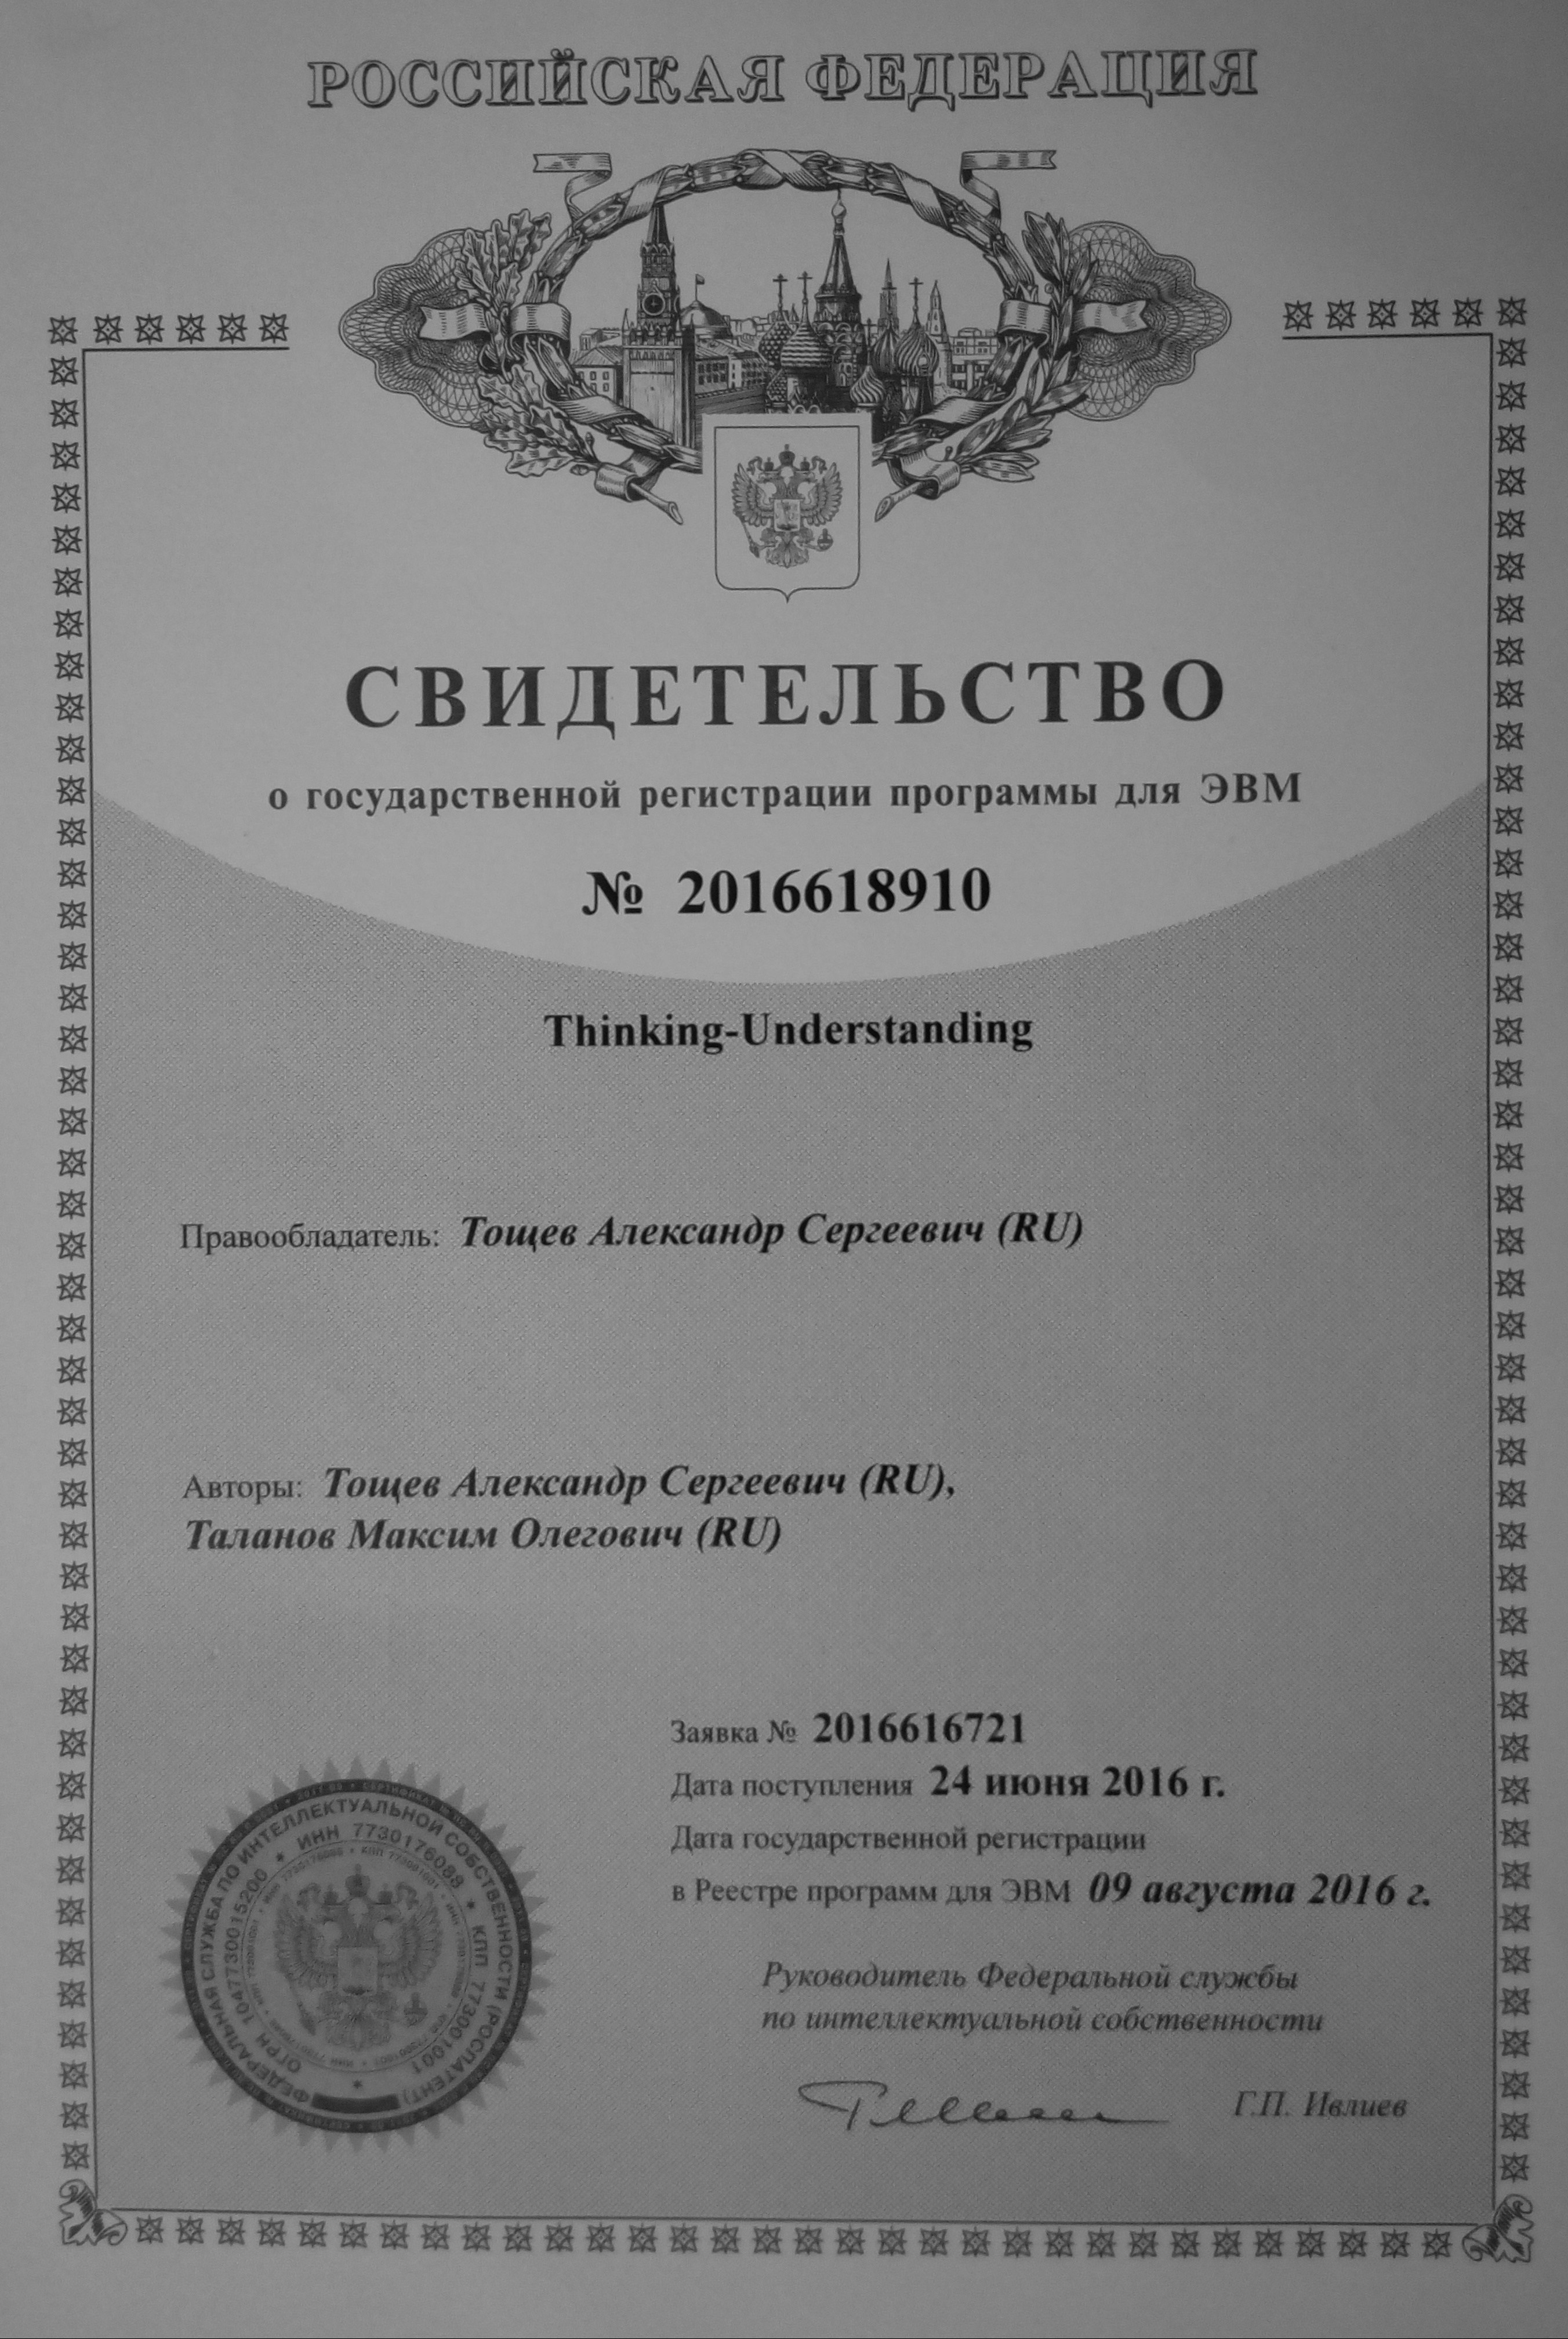
\includegraphics [scale=0.12] {RegistrationStatement}
  \caption{Свидетельство о регистрации} 
  \label{img:RegistrationStatement}  
\end{figure}



%=======================
%======APPENDIX G=======
%=======================
\clearpage
\chapter{Акт о внедрении}\label{AppendixG}


\begin{figure} [h] 
  \center
  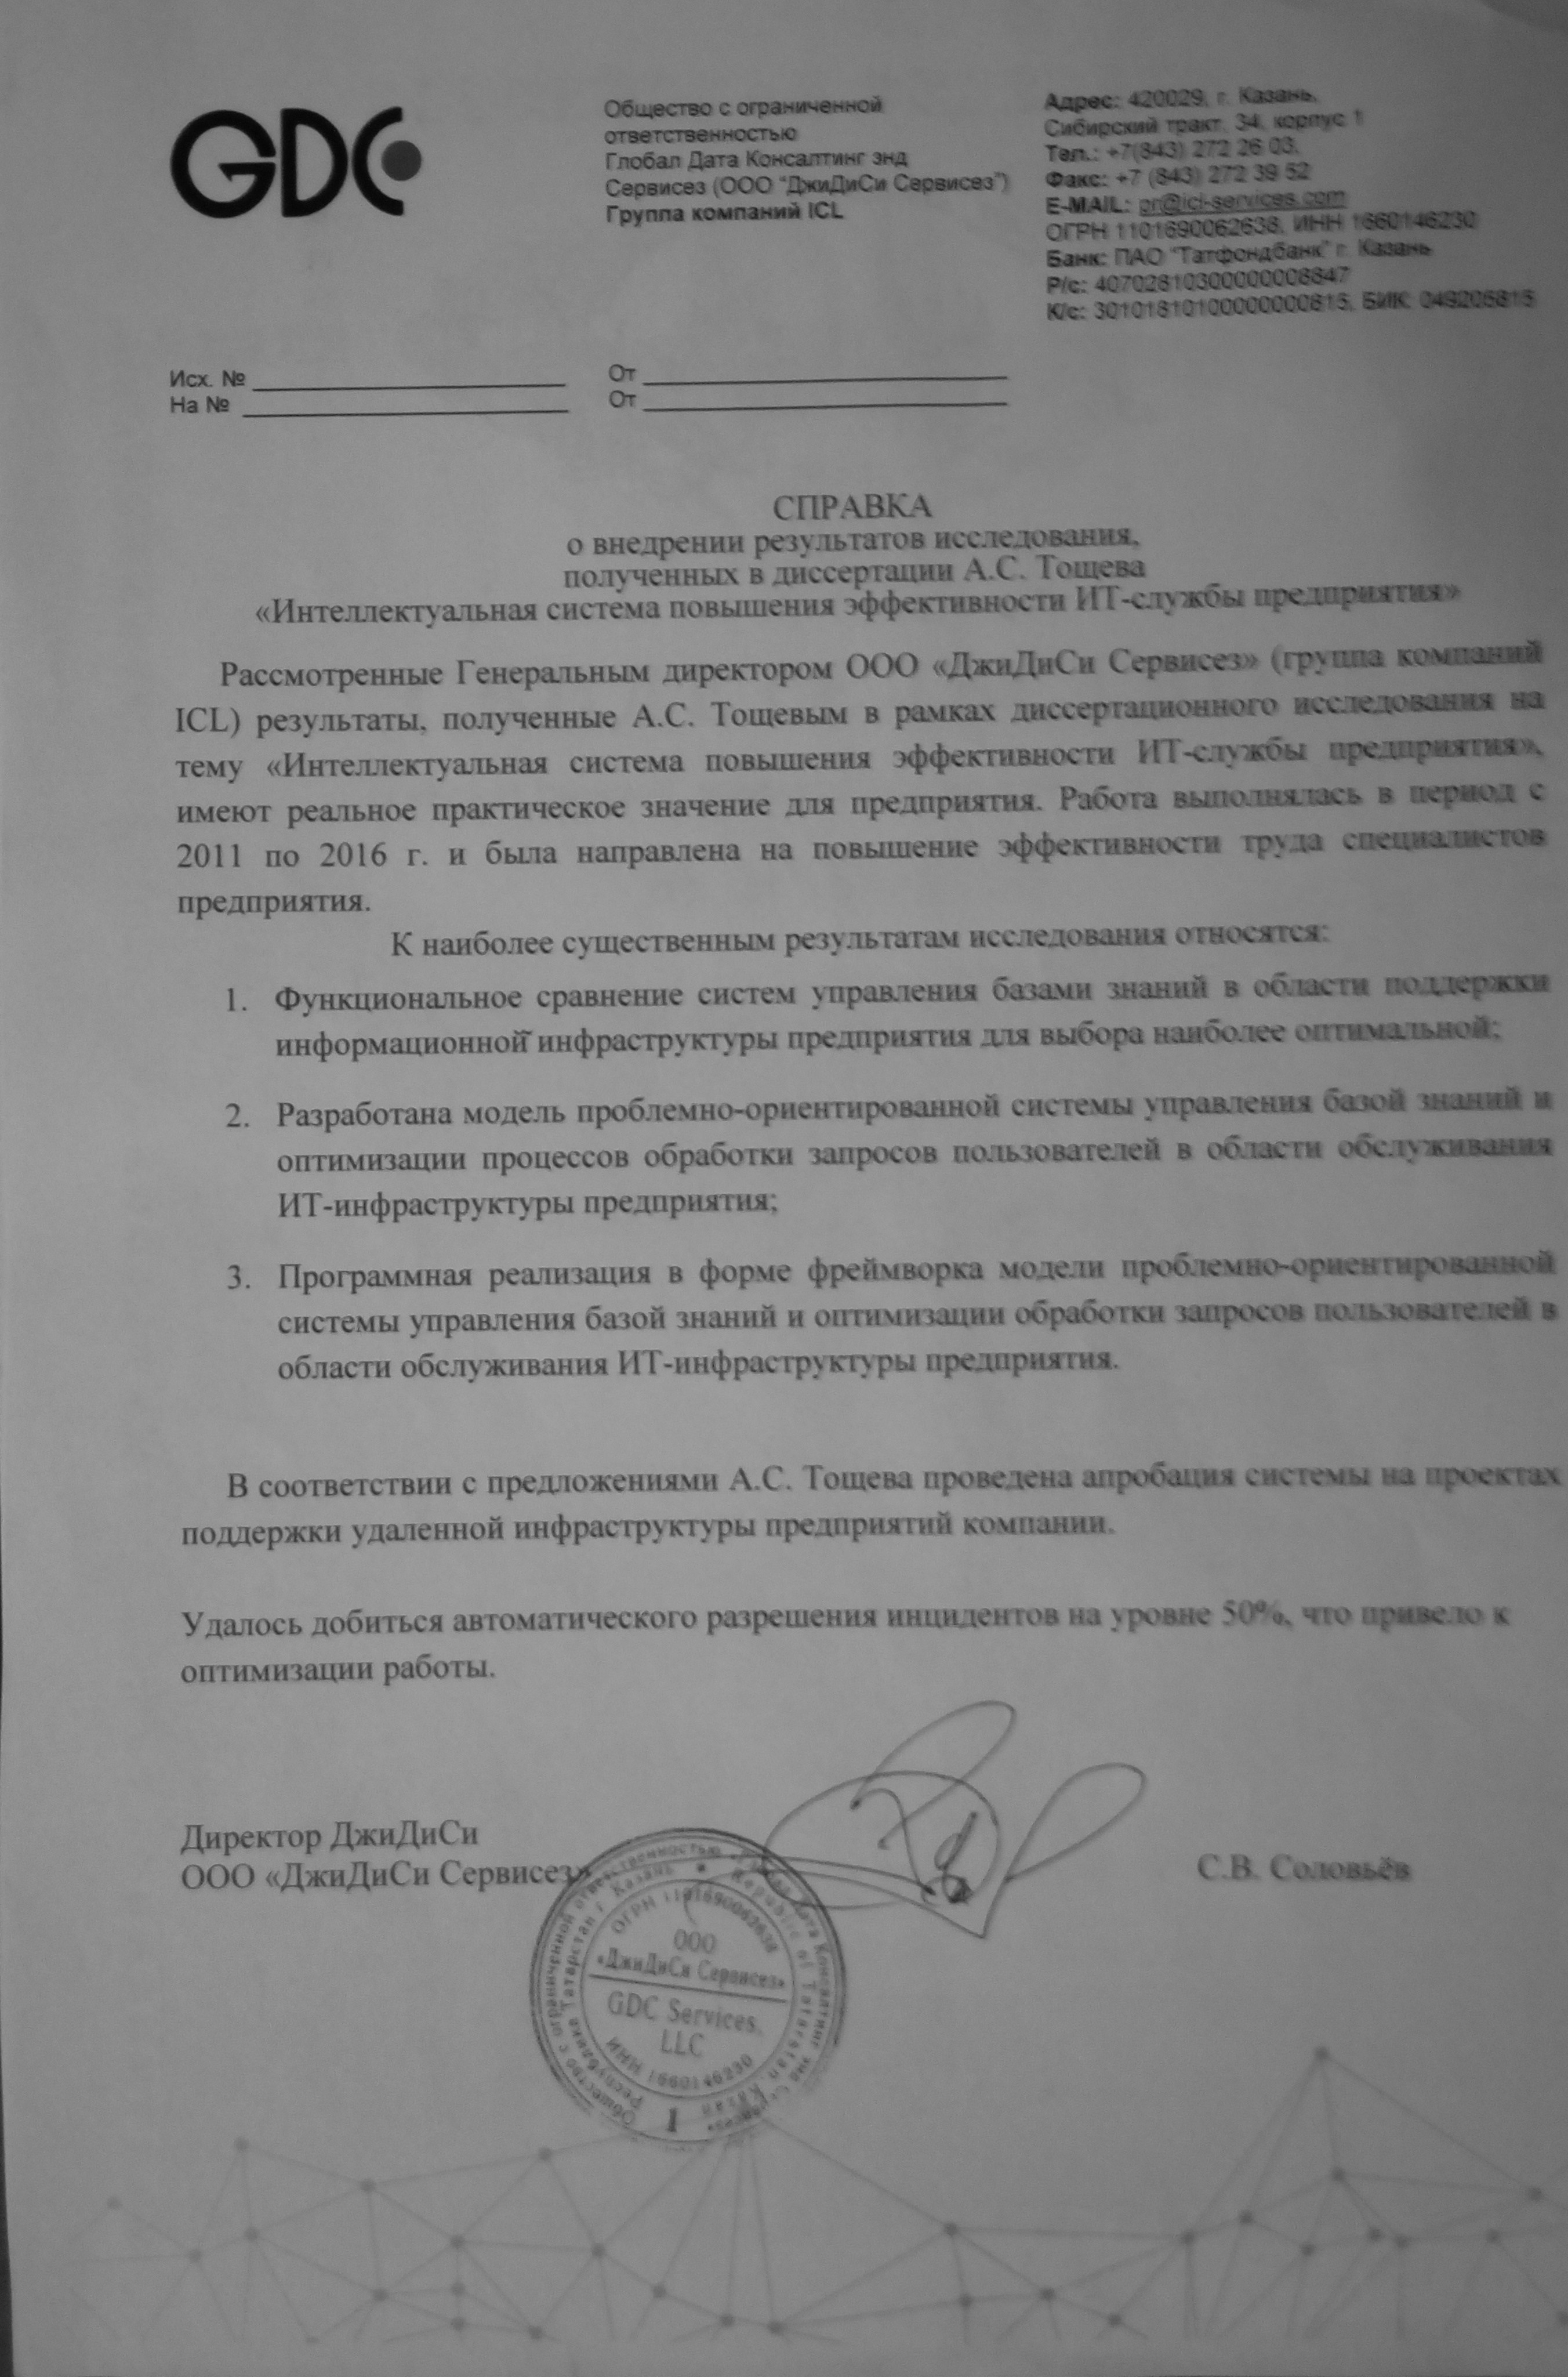
\includegraphics [scale=0.12] {ActVnedr}
  \caption{Акт о внедрении} 
  \label{img:ActVnedr}  
\end{figure}

        % Приложения

\end{document}
